\documentclass[12pt]{beamer}
\usepackage[utf8]{inputenc}
\usepackage[spanish]{babel}
\usepackage{graphicx}
\usepackage{amsmath}
\usepackage{booktabs}
\usepackage{multicol}
\usepackage{caption}
\usepackage{tikz}
\usepackage{amssymb}


\usetheme{Madrid}

\title[Proyecto Global Integrador]{
Control de Accionamiento de CA con
Motor Sincrónico de Imanes Permanentes}
\author[Quiroga, Armani]{\textbf{Integrantes: }\\Juan Quiroga, Matías Armani\\ \textbf{Profesor:}\\ Ing. Gabriel L. Julián}
\date{Febrero 2025}

\begin{document}

\frame{\titlepage}

\begin{frame}{Resumen}
Este trabajo desarrolla un sistema de control automático para un accionamiento eléctrico basado en un motor síncrono de imanes permanentes (PMSM), aplicado al control de un manipulador robótico de un grado de libertad. El proyecto integra modelado matemático, simulación dinámica y diseño de controladores, siguiendo los lineamientos establecidos para un sistema de lazo cerrado con control en cascada.

El análisis incluye un modelo dinámico no lineal del sistema físico, que abarca los subsistemas mecánico, electromagnético y térmico. Se diseñaron estrategias de control vectorial con desacoplamiento de torque y flujo magnético, utilizando un controlador PID optimizado para garantizar precisión en el seguimiento de consignas de posición y velocidad.
\end{frame}

% Slide 1: Introducción
\begin{frame}{Introducción}
\textbf{Objetivo:} Diseñar un sistema de control para un accionamiento basado en un motor síncrono de imanes permanentes (PMSM).
\begin{itemize}
    \item Modelado del sistema mecánico, electromagnético y térmico.
    \item Implementación de un controlador PID optimizado.
    \item Simulación en MATLAB/Simulink.
    \item Evaluación del desempeño bajo diferentes condiciones.
\end{itemize}
\end{frame}
%% CARGA MECÁNICA
\begin{frame}{Carga mecánica}
La ecuación que describe el sistema es:
\begin{equation}
        J_l \frac{d\omega_l}{dt} = T_q - b_l \omega_l - T_l(t); \quad T_l(t) = g \cdot k_l \cdot \sin(\theta_l(t)) + T_{ld}(t),
\label{eq:carga_mecanica}
\end{equation}

\begin{figure}[H]
    \centering
    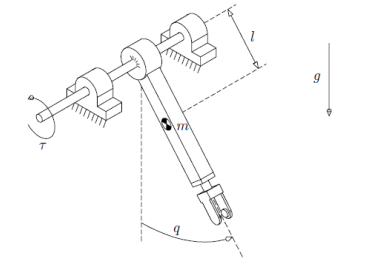
\includegraphics[width=0.55\textwidth]{Imagenes/brazo_robotico.png}
    \label{fig:brazo_robotico}
\end{figure}

\end{frame}

\begin{frame}{Carga mecánica}\scriptsize
\textbf{Parámetros} equivalentes \textit{variables} (\textit{valor nominal $\pm$ variación máx.}):

\begin{itemize}
    \item Coeficiente de fricción viscosa en la articulación:  
    \[
    b_l \approx (0.1 \pm 0.03) \frac{\text{N} \cdot \text{m}}{\text{rad/s}} \quad \text{(incertidumbre)}
    \]

    \item Masa del brazo manipulador:  
    \[
    m = 1.0 \text{ kg}
    \]

    \item Longitud e Inercia equivalente (centro de masa):  
    \[
    l_{cm} = 0.25 \text{ m}; \quad J_{cm} = 0.0208 \text{ kg}\cdot\text{m}^2
    \]

    \item Longitud total (extremo):  
    \[
    l_l = 0.50 \text{ m}
    \]

    \item Masa de \textit{Carga útil} en el extremo (\textit{variable}):  
    \[
    m_l = [0 \dots 1.5] \text{ kg}
    \]

    \item Momento de inercia total (a eje de rotación):  
    \[
    J_l = (m \cdot l_{cm}^2 + J_{cm}) + m_l \cdot l_l^2 = 0.0833 + [0 \dots 0.375] \text{ kg} \cdot \text{m}^2
    \]

    \item Coeficiente $k_l$ en Torque de carga $T_l(t)$, Ec.~\ref{eq:carga_mecanica}:  
    \[
    k_l = m \cdot l_{cm} + m_l \cdot l_l = 0.25 + [0 \dots 0.75] \text{ kg} \cdot \text{m}
    \]

    \item Torque recuperador gravitacional $g \cdot k_l \cdot \sin(\theta_l(t))$.
\end{itemize}

\end{frame}

\begin{frame}{Carga mecánica} \footnotesize
\textbf{Especificaciones de operación} (carga o perturbación adicional, por ejemplo \textit{contacto}, valor límite):

\begin{itemize}
    \item Torque de perturbación por contacto:  
    \[
    T_{ld}(t) \approx (0 \pm 5.0) \text{ N} \cdot \text{m} \quad \text{(asumir función escalón)}
    \]
\end{itemize}

Además, la posición angular \( \theta_l(t) \) del eje mecánico está relacionada con la velocidad angular mediante:
\begin{equation}
    \frac{d\theta_l(t)}{dt} = \omega_l(t) \iff \theta_l(t) = \int_{0}^{t} \omega_l(\xi) d\xi + \theta_l(0).
\end{equation}

donde:
\begin{itemize}
    \item \( \omega_l \): Velocidad angular de la articulación del brazo robótico.
    \item \( \theta_l(t) \): Posición angular de la articulación del brazo robótico.
\end{itemize}

\end{frame}

%% TREN DE TRANSMISIÓN

\begin{frame}{Tren de transmisión}
    Asumiendo un acoplamiento rígido, las relaciones entre las variables son:
\begin{equation}
\label{eq:transmision_velocidades}
    \omega_l(t) = \frac{1}{r} \omega_m(t),
\end{equation}
\begin{equation}
\label{eq:transmision_torques}
    T_q(t) = r T_d(t),
\end{equation}

donde:
\begin{itemize}
    \item \( r \): Relación de reducción del tren de transmisión.
    \item \( \omega_m(t) \): Velocidad angular del eje del motor.
    \item \( T_d(t) \): Torque de entrada al tren de transmisión.
    \item \( T_q(t) \): Torque de salida al tren de transmisión.
\end{itemize}

\textbf{Parámetro (constante):}
\begin{itemize}
    \item Relación de reducción total: \( r = 120.0 : 1 \).
\end{itemize}
\end{frame}


\begin{frame}{Tren de transmisión}
\textbf{Especificaciones de operación (valores límite, no sobrepasar):}
\begin{itemize}\footnotesize
    \item Velocidad nominal (salida): \( n_{1,\text{nom}} = 60 \, \text{rpm} \) (\( \omega_{1,\text{nom}} = 6.28 \, \text{rad/s} \)).
    \item Torque nominal (salida): \( T_{q,\text{nom}} = 17.0 \, \text{N.m} \) (régimen continuo o rms).
    \item Torque pico (salida): \( T_{q,\text{max}} = 45.0 \, \text{N.m} \) (corta duración, \underline{aceleración}).
\end{itemize}

    \begin{figure}[H]
        \centering
        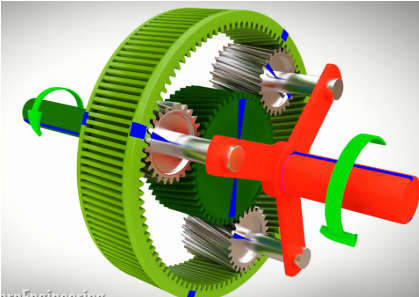
\includegraphics[width=0.55\textwidth]{Imagenes/tren_transmision.png}
        \label{fig:tren_transmision}
    \end{figure}
\end{frame}

%% MAQUINA ELECTRICA
\begin{frame}{Máquina Eléctrica PMSM}
El modelo matemático equivalente del subsistema mecánico del rotor de la máquina eléctrica (referido a Estator estacionario = fijo al sistema inercial de referencia) se describe mediante la ecuación:
\begin{equation}
\label{eq:subsistema_mecanico_maquina_pmsm}
    J_m \frac{d\omega_m}{dt} = T_m - b_m \omega_m - T_d,
\end{equation}

\begin{equation}
    \frac{d\theta_m(t)}{dt} = \omega_m(t) \iff \theta_m(t) = \int_{0}^{t} \omega_m(\xi) d\xi + \theta_m(0).
\end{equation}

donde:
\begin{itemize}
    \item $J_m$: Momento de inercia (motor y caja).
    \item $\omega_m$: Velocidad angular del motor.
    \item $T_m$: Torque electromagnético generado por el motor.
    \item $b_m$: Coeficiente de fricción viscosa (motor y caja).
\end{itemize}
\end{frame}



%% Subsistema Mecánico Completo
\begin{frame}{Subsistema Mecánico Completo}
    Sustituyendo \( \omega_l(t) \) de (Ec.~\ref{eq:transmision_velocidades}) y \( T_q(t) \) de (Ec.~\ref{eq:transmision_torques}) en (Ec.~\ref{eq:carga_mecanica}):
    \begin{equation}
        \frac{J_l}{r} \frac{d\omega_m(t)}{dt} = r T_d(t) - \frac{b_l}{r} \omega_m(t) - T_l(t),
    \end{equation}
    Despejando \( T_d(t) \) y reemplazando \( T_l(t) \) por su expresión equivalente:
    \begin{equation}
    \label{eq:expresion_Td_despejado}
        T_d(t) = \frac{J_l}{r^2} \frac{d\omega_m}{dt} + \frac{b_l}{r^2} \omega_m + \frac{1}{r} \left(g \cdot k_l \cdot \sin\left(\frac{\theta_m(t)}{r}\right) + T_{ld}(t)\right),
    \end{equation}
    Reemplazando \( T_d(t) \) de (Ec.~\ref{eq:expresion_Td_despejado}) en (Ec.~\ref{eq:subsistema_mecanico_maquina_pmsm}):
    \begin{equation}
        J_{\text{eq}} \frac{d\omega_m}{dt} = -b_{\text{eq}} \omega_m + T_m - \frac{1}{r} \left(g \cdot k_l \cdot \sin\left(\frac{\theta_m(t)}{r}\right) + T_{ld}(t)\right),
    \end{equation}
    con:
    \begin{equation}
        J_{\text{eq}} = J_m + \frac{J_l}{r^2}, \quad
        b_{\text{eq}} = b_m + \frac{b_l}{r^2}, \quad
        \theta_l(t) = \frac{\theta_m(t)}{r}.
    \end{equation}
\end{frame}


\begin{frame}{Subsistema Mecánico Completo}\footnotesize
    \textbf{Modelo matemático equivalente:}
    \begin{equation}
        \resizebox{0.9\hsize}{!}{$
        \dot{\theta}_m(t) = \omega_m(t), \quad
        \dot{\omega}_m(t) = -\frac{b_{\text{eq}}}{J_{\text{eq}}} \omega_m(t) 
        - \frac{g \cdot k_l}{J_{\text{eq}} r} \sin\left(\frac{\theta_m(t)}{r}\right) 
        + \frac{1}{J_{\text{eq}}} T_m(t).
        $}
    \end{equation}
    \textbf{Parámetros:}
    \begin{itemize}\footnotesize
        \item \( J_{\text{eq}} = J_m + \frac{J_l}{r^2} \), \( b_{\text{eq}} = b_m + \frac{b_l}{r^2} \).
        \item Relación entre ángulos: \( \theta_l(t) = \frac{\theta_m(t)}{r} \).
    \end{itemize}
    \textbf{Ecuaciones de estado:}
    \begin{equation}
    \left\{
    \begin{aligned}
        \dot{\theta}_m(t) &= \omega_m(t), \\
        \dot{\omega}_m(t) &= -\frac{b_{\text{eq}}}{J_{\text{eq}}} \omega_m(t) - \frac{g \cdot k_l}{J_{\text{eq}} r} \cdot \sin\left(\frac{\theta_m(t)}{r}\right) + \frac{1}{J_{\text{eq}}} T_m(t) - \frac{1}{J_{\text{eq}} r} T_{ld}(t), \\
        y(t) &= \theta_m(t).
    \end{aligned}
    \right.
    \end{equation}
\end{frame}

\begin{frame}{Subsistema Mecánico Completo}\footnotesize

\textbf{Forma matricial:}
\begin{equation}
\left\{
\begin{aligned}
\begin{bmatrix}
    \dot{\theta}_m(t) \\
    \dot{\omega}_m(t)
\end{bmatrix}
&=
\underbrace{
\begin{bmatrix}
    \omega_m(t) \\
    -\frac{g \cdot k_l}{J_{\text{eq}} r} \cdot \sin\left(\frac{\theta_m(t)}{r}\right) -\frac{b_{\text{eq}}}{J_{\text{eq}}} \cdot \omega_m(t) 
\end{bmatrix}
}_{f(\theta_m(t),\omega_m(t))}
+
\begin{bmatrix}
    0 & 0 \\
    \frac{1}{J_{\text{eq}}} & -\frac{1}{J_{\text{eq}} r}
\end{bmatrix}
\begin{bmatrix}
    T_m(t) \\
    T_{ld}(t)
\end{bmatrix}, \\
y(t) &=
\begin{bmatrix}
    1 & 0
\end{bmatrix}
\begin{bmatrix}
    \theta_m(t) \\
    \omega_m(t)
\end{bmatrix}.
\end{aligned}
\right.
\end{equation}
    \begin{figure}[H]
        \centering
        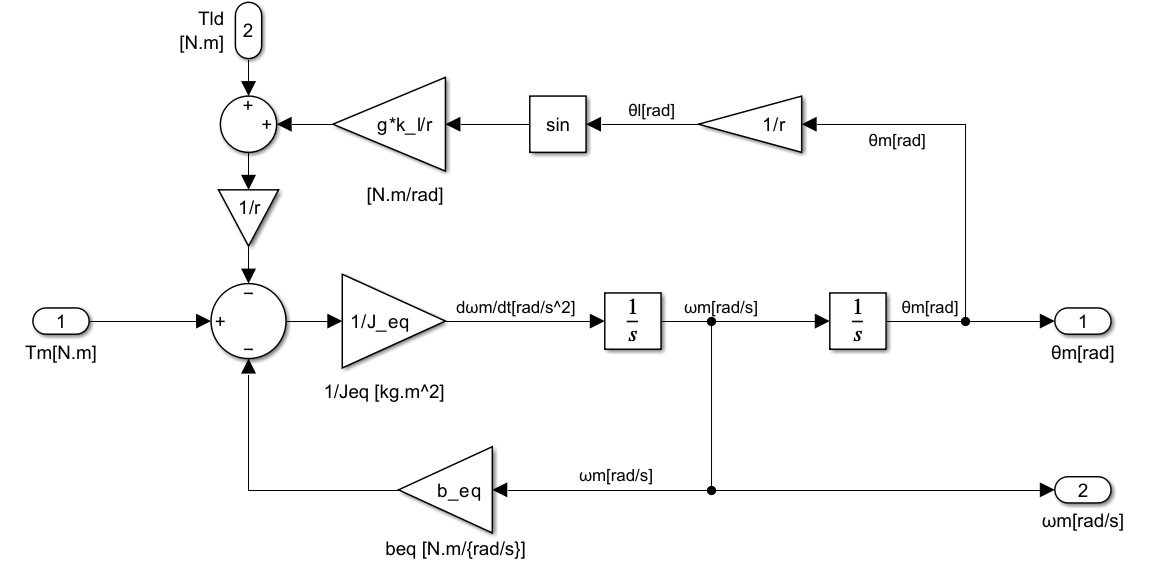
\includegraphics[width=0.6\textwidth]{Imagenes/bloque_subsistema_mecanico.png}
        \caption{Diagrama desagregado del subsistema mecánico completo.}
    \end{figure}
\end{frame}

%% Modelo dinámico del sistema físico completo
\begin{frame}{Modelo Dinámico del Sistema Físico Completo}\footnotesize
\textbf{Modelo global No Lineal:}
    \begin{figure}[H]
        \centering
        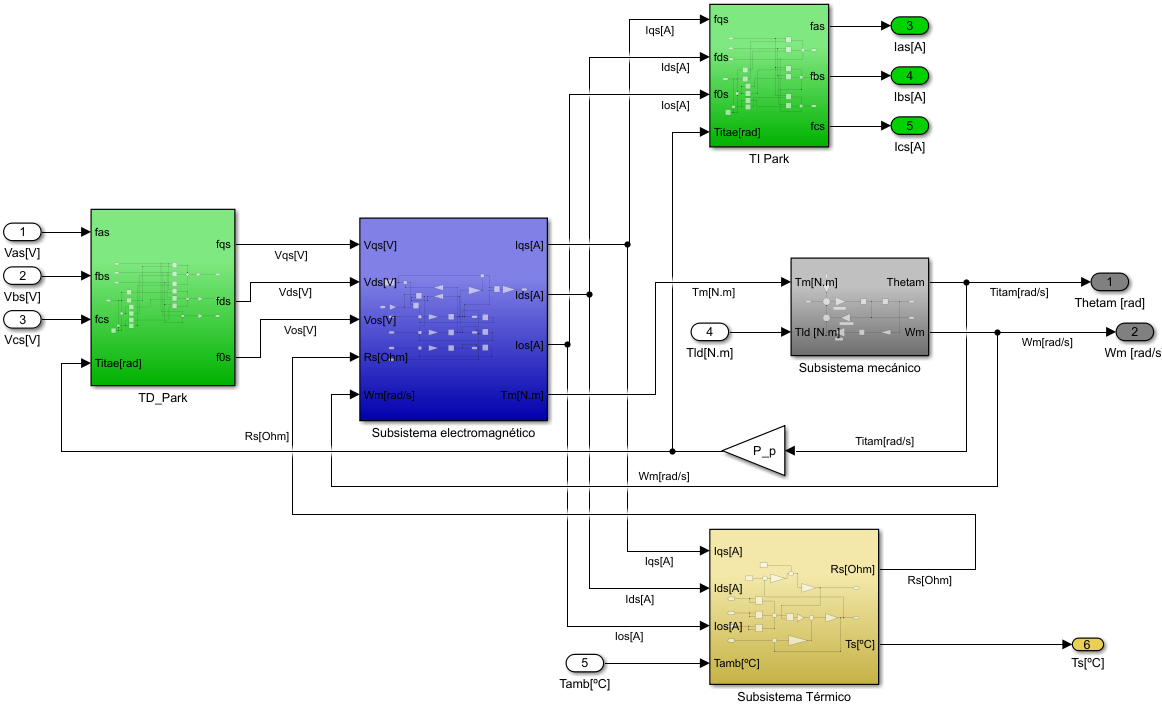
\includegraphics[width=0.9\textwidth]{Imagenes/Diagrama_Global_NoLineal.png}
        \caption{Diagrama de bloques desagregado del sistema global no lineal.}
    \end{figure}
\end{frame}

%% Transformaciones de Park
\begin{frame}{Transformaciones de Park}\footnotesize
\textbf{Transformación de Park Directa:}
\begin{equation}
\begin{bmatrix}
    f_{qs}^r(t) \\ f_{ds}^r(t) \\ f_{0s}(t)
\end{bmatrix} = \frac{2}{3}
\begin{bmatrix}
    \cos\theta_r(t) & \cos(\theta_r(t) - \frac{2\pi}{3}) & \cos(\theta_r(t) + \frac{2\pi}{3}) \\
    \sin\theta_r(t) & \sin(\theta_r(t) - \frac{2\pi}{3}) & \sin(\theta_r(t) + \frac{2\pi}{3}) \\
    \frac{1}{2} & \frac{1}{2} & \frac{1}{2}
\end{bmatrix}
\begin{bmatrix}
    f_{as}(t) \\ f_{bs}(t) \\ f_{cs}(t)
\end{bmatrix}
\end{equation}

\textbf{Transformación de Park Inversa:}
\begin{equation}
\begin{bmatrix}
    f_{as}(t) \\ f_{bs}(t) \\ f_{cs}(t)
\end{bmatrix} =
\begin{bmatrix}
    \cos\theta_r(t) & \sin\theta_r(t) & 1 \\
    \cos(\theta_r(t) - \frac{2\pi}{3}) & \sin(\theta_r(t) - \frac{2\pi}{3}) & 1 \\
    \cos(\theta_r(t) + \frac{2\pi}{3}) & \sin(\theta_r(t) + \frac{2\pi}{3}) & 1
\end{bmatrix}
\begin{bmatrix}
    f_{qs}^r(t) \\ f_{ds}^r(t) \\ f_{0s}(t)
\end{bmatrix}
\end{equation}

\begin{figure}[h]
    \centering
    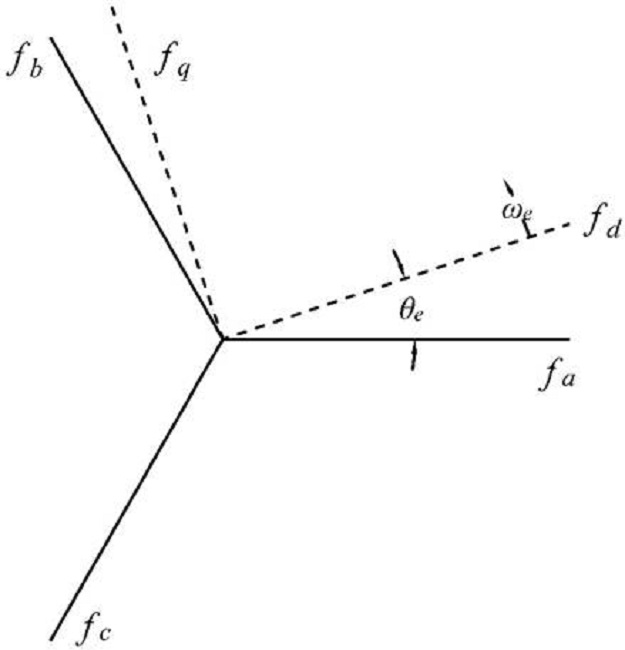
\includegraphics[width=0.2\textwidth]{Imagenes/CoordVirtuales.jpg}
    \caption{Ejes absolutos de fases \textbf{a, b} y \textbf{c} del estator y ejes \textbf{q} y \textbf{d} fijos a rotor.}
\end{figure}
\end{frame}

\begin{frame}{Transformaciones de Park}
    \footnotesize
    \captionsetup{font=footnotesize} % Configuración para achicar captions
    \begin{figure}[H]
        \centering
        \begin{minipage}[t]{0.35\textwidth}
            \centering
            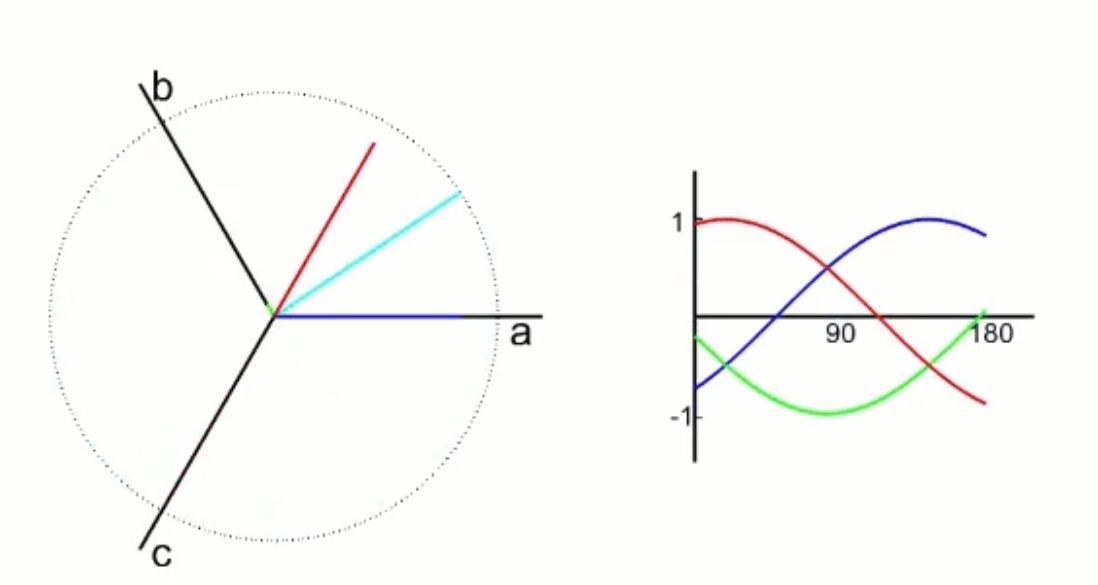
\includegraphics[width=\textwidth]{Imagenes/SistTrifasico(marcoABC).png}
            \caption{Componentes de un sistema trifásico (de un marco abc).}
        \end{minipage}
        \hfill
        \begin{minipage}[t]{0.35\textwidth}
            \centering
            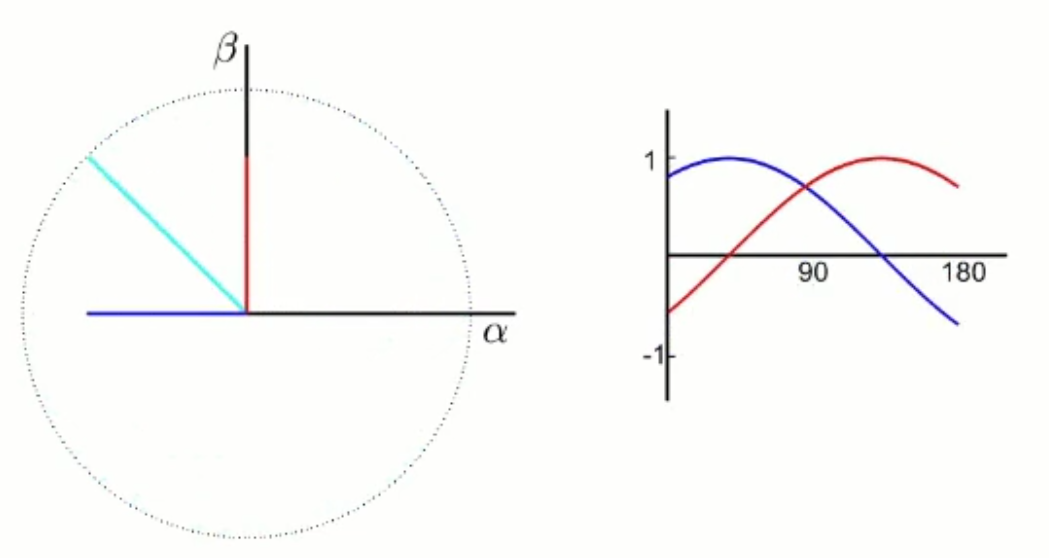
\includegraphics[width=\textwidth]{Imagenes/TransformadaClark.png}
            \caption{Señales resultantes de la transformación de Clarke (\(\alpha \beta\)).}
        \end{minipage}
        \vspace{0.25cm}
        \begin{minipage}[t]{0.35\textwidth}
            \centering
            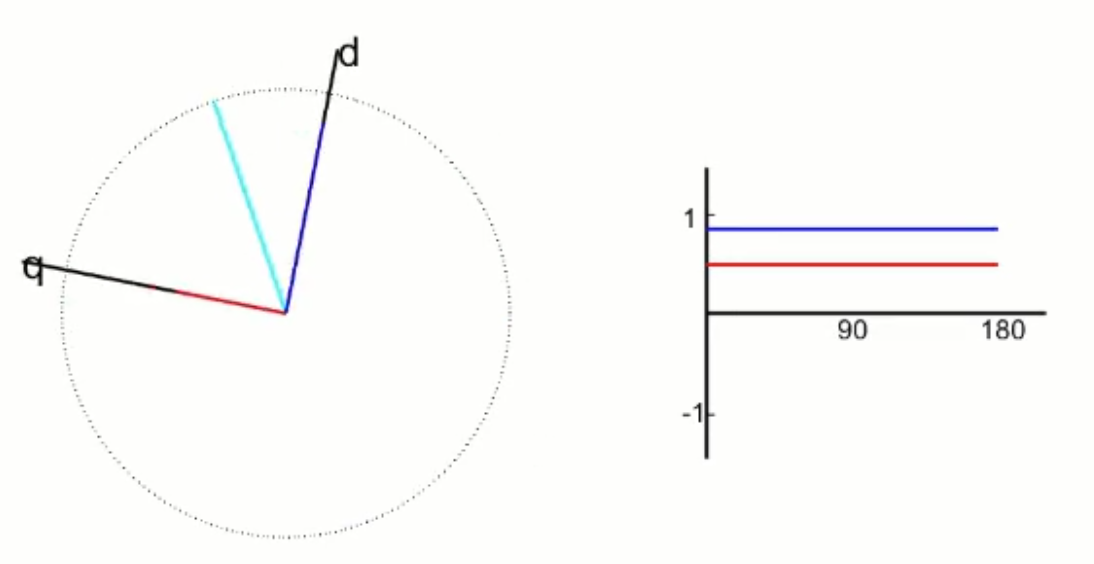
\includegraphics[width=\textwidth]{Imagenes/TransformadaPark.png}
            \caption{Señales resultantes de la transformación de Park (dq).}
        \end{minipage}
    \end{figure}
\end{frame}

\begin{frame}{Transformaciones de Park}\footnotesize
    \textbf{Transformación de Park Directa:}  
    \begin{figure}[h]
        \centering
        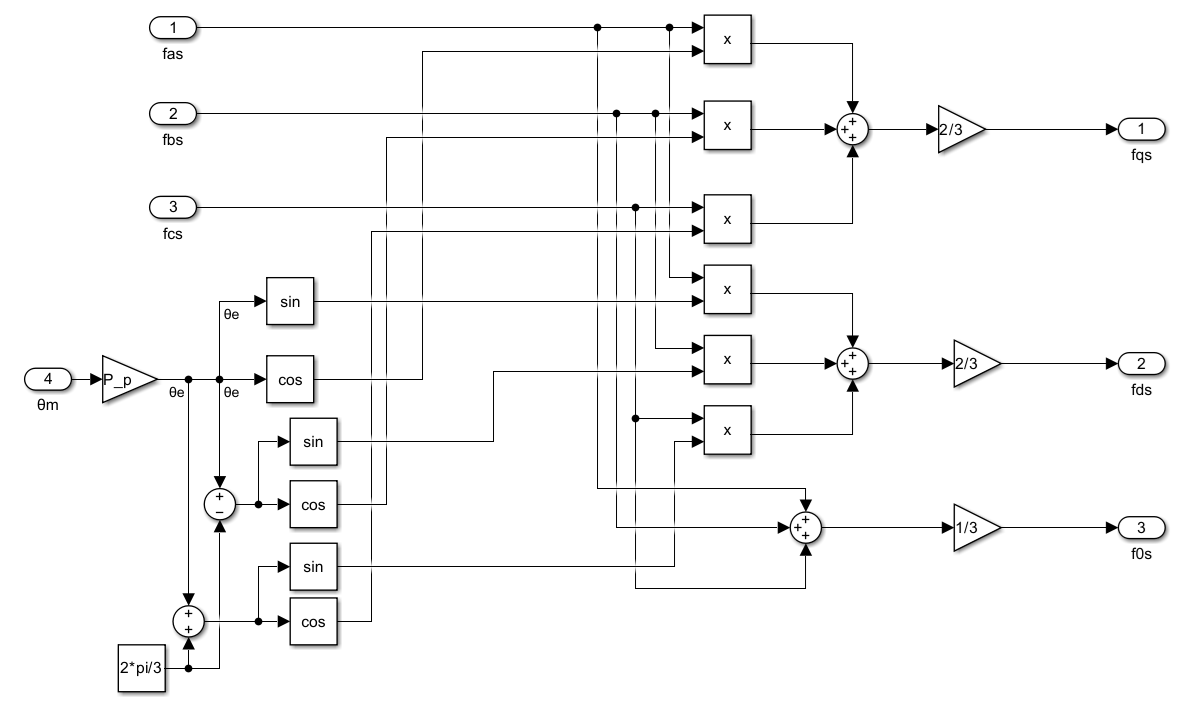
\includegraphics[width=0.9\textwidth]{Imagenes/ParkDirecta.png}
        \caption{Diagrama de bloques de la transformación directa de Park.}
    \end{figure}
\end{frame}

\begin{frame}{Transformaciones de Park}\footnotesize
    \textbf{Transformación de Park Inversa:}   
    \begin{figure}[h]
        \centering
        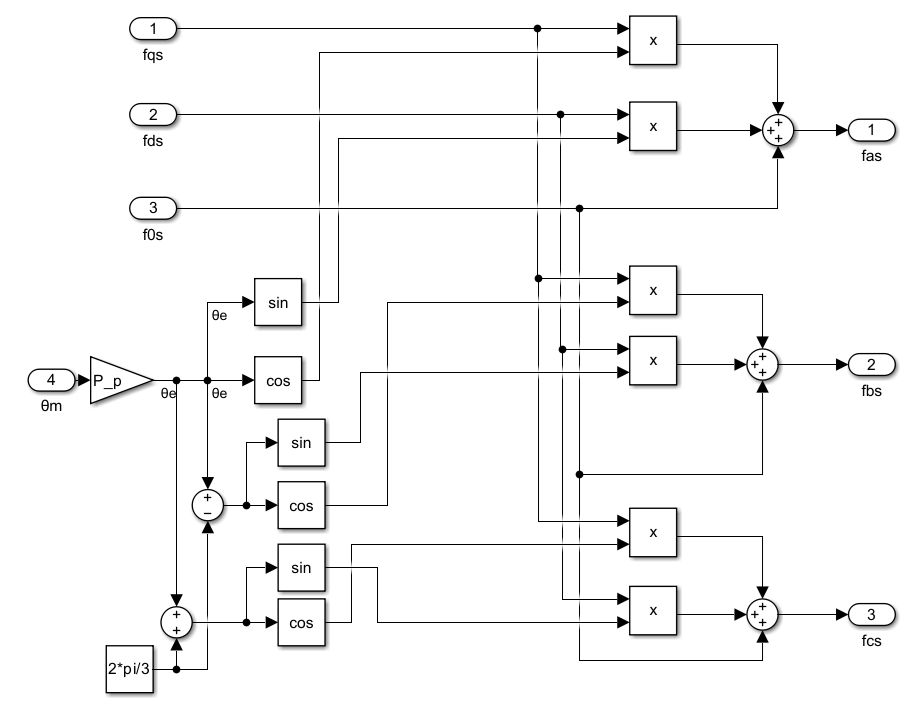
\includegraphics[width=0.72\textwidth]{Imagenes/ParkInversa.png}
        \caption{Diagrama de bloques de la transformación inversa de Park.}
    \end{figure}
\end{frame}


%% Subsistema Electromagnético
\begin{frame}{Subsistema Electromagnético}\footnotesize
    \textbf{Coordenadas eléctricas de qd0 fijas a rotor (sincrónico):}
    \begin{equation}
    \frac{d\theta_r(t)}{dt} \equiv \omega_r(t) \iff \theta_r(t) = \int_{0}^{t} \omega_r(\xi) \, d\xi + \theta_r(0)
    \end{equation}
    \begin{equation}
    \theta_r(t) \equiv P_p \cdot \theta_m(t) \therefore \omega_r(t) = P_p \cdot \omega_m(t)
    \end{equation}
    \textbf{Balance de tensiones eléctricas en cada fase:}
    \begin{equation}
    \left\{
    \begin{aligned}
        v_{as}(t) &= r_s i_{as} + \frac{d\lambda_{as}}{dt}, \\
        v_{bs}(t) &= r_s i_{bs} + \frac{d\lambda_{bs}}{dt}, \\
        v_{cs}(t) &= r_s i_{cs} + \frac{d\lambda_{cs}}{dt}.
    \end{aligned}
    \right.
    \end{equation}
\end{frame}

\begin{frame}{Subsistema Electromagnético}
    \footnotesize
    \textbf{Ecuación Vectorial de Tensión del Estator en qd0:}
    \[
    \vec{v}^\theta_{qd0}(t) =
    \begin{bmatrix}
        r_s & 0 & 0 \\
        0 & r_s & 0 \\
        0 & 0 & r_s
    \end{bmatrix}
    \cdot \vec{i}^\theta_{qd0}(t) + 
    L \cdot \frac{d\vec{i}^\theta_{qd0}(t)}{dt} +
    \frac{d\Theta(t)}{dt} \cdot
    \begin{bmatrix}
        0 & 1 & 0 \\
        -1 & 0 & 0 \\
        0 & 0 & 0
    \end{bmatrix}
    \cdot \vec{\lambda}^\theta_{qd0}(t)
    \]
    \begin{equation}
    \left\{
    \begin{aligned}
    v^\theta_{qs}(t) &= r_s \cdot i^\theta_{qs}(t) + \frac{d\lambda^\theta_{qs}(t)}{dt} + \frac{d\Theta(t)}{dt} \cdot \lambda^\theta_{ds}(t), \\
    v^\theta_{ds}(t) &= r_s \cdot i^\theta_{ds}(t) + \frac{d\lambda^\theta_{ds}(t)}{dt} - \frac{d\Theta(t)}{dt} \cdot \lambda^\theta_{qs}(t), \\
    v^\theta_{0s}(t) &= r_s \cdot i^\theta_{0s}(t) + \frac{d\lambda^\theta_{0s}(t)}{dt}.
    \end{aligned}
    \right.
    \end{equation}
    \textbf{Expresiones de los flujos concatenados en qd0}
    \[
    \left\{
    \begin{aligned}
        \lambda^{r}_{qs}(t) &= L_q \cdot i^{r}_{qs}(t), \\
        \lambda^{r}_{ds}(t) &= L_d \cdot i^{r}_{ds}(t) + \lambda_m, \\
        \lambda^{r}_{0s}(t) &= L_0 \cdot i^{r}_{0s}(t).
    \end{aligned}
    \right.
    \]
\end{frame}

\begin{frame}{Subsistema Electromagnético}\footnotesize
    \textbf{Sistema de Ecuaciones de Tensiones en coordenadas qd0}
    \begin{equation}
    \left\{
    \begin{aligned}
        v_{qs}^r(t) &= R_s(t) i_{qs}^r(t) + L_q \frac{d i_{qs}^r(t)}{dt} + \big(\lambda_m' + L_d i_{ds}^r(t)\big) \omega_r(t), \\
        v_{ds}^r(t) &= R_s(t) i_{ds}^r(t) + L_d \frac{d i_{ds}^r(t)}{dt} - L_q i_{qs}^r(t) \omega_r(t), \\
        v_{0s}^r(t) &= R_s(t) i_{0s}^r(t) + L_{ls} \frac{d i_{0s}^r(t)}{dt}, \\
        T_m(t) &= \frac{3}{2} P_p \lambda_m' i_{qs}^r(t) + \frac{3}{2} P_p (L_d - L_q) i_{ds}^r(t) i_{qs}^r(t).
    \end{aligned}
    \right.
    \label{eq:SubsistemaElectromagnetico}
    \end{equation}
    \textbf{Expresiones para las derivadas de las corrientes en qd0}
    \begin{equation}
    \left\{
    \begin{aligned}
        \frac{d i_{qs}^r(t)}{dt} &= \frac{1}{L_q} \Big( v_{qs}^r(t) - R_s(t) i_{qs}^r(t) - \big(\lambda_m' + L_d i_{ds}^r(t)\big) \omega_r(t) \Big), \\
        \frac{d i_{ds}^r(t)}{dt} &= \frac{1}{L_d} \Big( v_{ds}^r(t) - R_s(t) i_{ds}^r(t) + L_q i_{qs}^r(t) \omega_r(t) \Big), \\
        \frac{d i_{0s}^r(t)}{dt} &= \frac{1}{L_{ls}} \Big( v_{0s}^r(t) - R_s(t) i_{0s}^r(t) \Big).
    \end{aligned}
    \right.
    \end{equation}
\end{frame}

\begin{frame}{Subsistema Electromagnético}\footnotesize
    \begin{figure}[h]
        \centering
        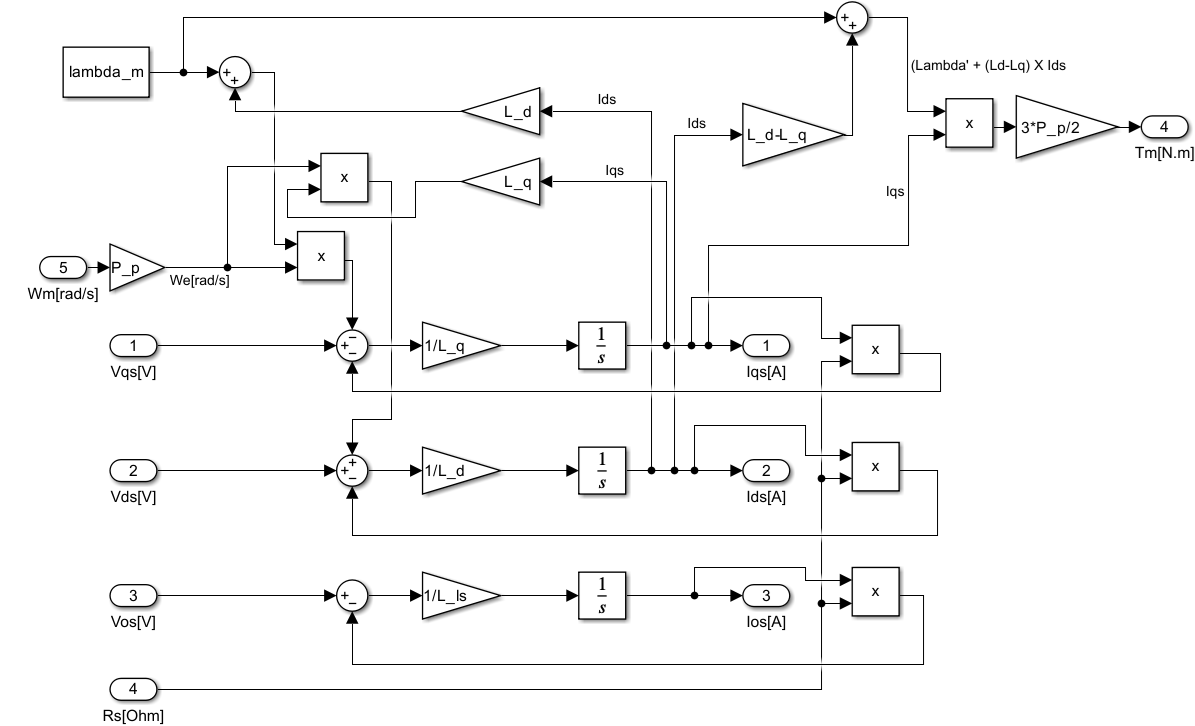
\includegraphics[width=0.83\textwidth]{Imagenes/BloquesSistElectromagnetico.png}
        \caption{Diagrama de bloques desagregado del subsistema electromagnético.}
    \end{figure}
\end{frame}

%% Subsistema Térmico
\begin{frame}{Subsistema térmico}\footnotesize
    La resistencia de los bobinados del estator varía con la temperatura del bobinado (\(T_s^\circ(t)\)) de acuerdo con la siguiente ecuación:
    
    \begin{equation}
    R_s(T_s^\circ(t)) = R_{s, \text{REF}} \cdot \Big( 1 + \alpha_\text{cu} \cdot (T_s^\circ(t) - T_{s, \text{REF}}) \Big),
    \end{equation}  

    \begin{figure}[h]
        \centering
        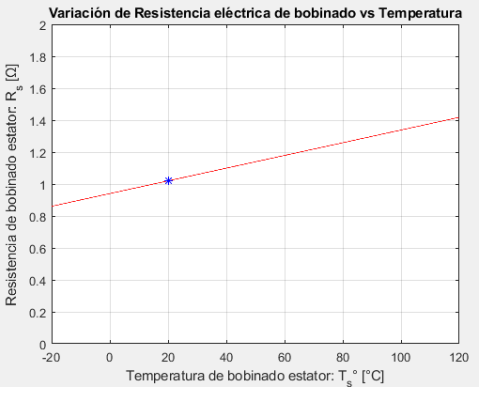
\includegraphics[width=0.45\textwidth]{Imagenes/Variacion_resistencia_temperatura.png}
        \caption{Comportamiento lineal de incremento de la resistencia con la temperatura.}
    \end{figure}
\end{frame}

\begin{frame}{Subsistema térmico}\footnotesize
    \textbf{Potencia disipada real en coordenadas abc:}
    \begin{equation}
    P_{\text{perd, abc}}(t) = R_s(t) \cdot \Big( i_{as}^2(t) + i_{bs}^2(t) + i_{cs}^2(t) \Big)
    \end{equation}
    \textbf{Potencia equivalente virtual en coordenadas qd0:}
    \begin{equation}
    P_{\text{perd, qd0}}(t) = \frac{3}{2} \cdot R_s(t) \cdot \Big( i_{qs}^r(t)^2 + i_{ds}^r(t)^2 + 2 \cdot i_{0s}^r(t)^2 \Big)
    \end{equation}
    \textbf{Balance energético:}
    \begin{equation}
    \frac{dT_s(t)}{dt} = \frac{1}{C_{ts}} \cdot \Big( P_{\text{perd}}(t) - \frac{1}{R_{ts-\text{amb}}} \big( T_s(t) - T_{\text{amb}} \big) \Big)
    \end{equation}
\begin{equation}
\label{eq:subsistema_termico}
\begin{split}
    \frac{dT_s(t)}{dt} = \frac{1}{C_{ts}} \Big[ &\frac{3}{2} \cdot R_s(t) \cdot \Big( i_{qs}^r(t)^2 + i_{ds}^r(t)^2 + 2 \cdot i_{0s}^r(t)^2 \Big) \\
    &- \frac{1}{R_{ts-\text{amb}}} \big( T_s(t) - T_{\text{amb}} \big) \Big]
\end{split}
\end{equation}
\end{frame}


\begin{frame}{Subsistema Térmico}
\begin{figure}[h]
    \centering
    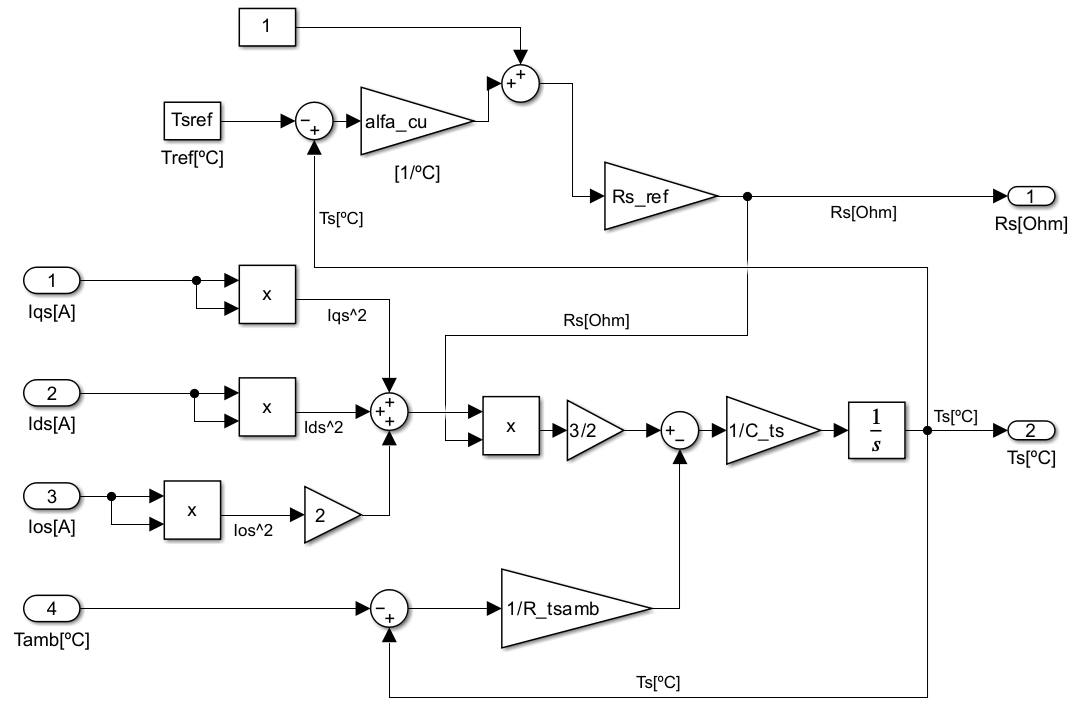
\includegraphics[width=0.9\textwidth]{Imagenes/BloquesSistTermico.png}
    \caption{Diagrama de bloques desagregado del subsistema térmico.}
\end{figure}
\end{frame}


%% Modelo Dinámico Global No Lineal (NL)
\begin{frame}{Modelo Dinámico Global No Lineal (NL)}
    \scriptsize % Reducir aún más el tamaño de fuente
    \begin{equation}
    \left\{
    \begin{aligned}
    \dot{\theta}_m(t) &= \omega_m(t), \\
    \dot{\omega}_m(t) &= \frac{1}{J_{eq}} \Bigg[ \frac{3}{2} P_p \Big( \lambda_m' i_{qs}^r(t) + (L_d - L_q) i_{ds}^r(t) i_{qs}^r(t) \Big) \\
    &\quad - b_{eq} \omega_m(t) - g \cdot k_l \sin\Bigg(\frac{\theta_m(t)}{r}\Bigg) - \frac{1}{r} T_{ld}(t) \Bigg], \\
    \frac{d i_{qs}^r(t)}{dt} &= \frac{1}{L_q} \Big( v_{qs}^r(t) - R_s(t) i_{qs}^r(t) - (\lambda_m' + L_d i_{ds}^r(t)) P_p \cdot \omega_m(t) \Big), \\
    \frac{d i_{ds}^r(t)}{dt} &= \frac{1}{L_d} \Big( v_{ds}^r(t) - R_s(t) i_{ds}^r(t) + L_q i_{qs}^r(t) P_p \cdot \omega_m(t) \Big), \\
    \frac{d i_{0s}(t)}{dt} &= \frac{1}{L_{ls}} \Big( v_{0s}(t) - R_s(t) i_{0s}(t) \Big), \\
    \frac{d T_s(t)}{dt} &= \frac{1}{C_{ts}} \Bigg[ \frac{3}{2} R_s(t) \Big( (i_{qs}^r(t))^2 + (i_{ds}^r(t))^2 + 2 \cdot (i_{0s}(t))^2 \Big) \\
    &\quad - \frac{1}{R_{ts-amb}} \big( T_s(t) - T_{\text{amb}} \big) \Bigg].
    \end{aligned}
    \right.
    \end{equation}
\end{frame}

\begin{frame}{Modelo Dinámico Global No Lineal (NL)}
    \tiny % Reducir aún más el tamaño del texto
    \begin{equation}
    \left\{
    \begin{aligned}
    \begin{bmatrix}
        \dot{\theta}_m(t) \\
        \dot{\omega}_m(t) \\
        \dot{i_{qs}^r}(t) \\
        \dot{i_{ds}^r}(t) \\
        \dot{i_{0s}^r}(t) \\
        \dot{T}_s(t)
    \end{bmatrix}
    &=
    \underbrace{
    \begin{bmatrix}
        \omega_m(t) \\
        \frac{1}{J_{eq}} \Big[ \frac{3}{2} P_p \big( \lambda_m' i_{qs}^r(t) + (L_d - L_q) i_{ds}^r(t) i_{qs}^r(t) \big) - b_{eq} \omega_m(t) - g \cdot k_l \sin\big(\frac{\theta_m(t)}{r}\big) \Big] \\
        \frac{1}{L_q} \Big(- R_s(t) i_{qs}^r(t) - (\lambda_m' + L_d i_{ds}^r(t)) P_p \omega_m(t) \Big) \\
        \frac{1}{L_d} \Big( - R_s(t) i_{ds}^r(t) + L_q i_{qs}^r(t) P_p \omega_m(t) \Big) \\
        \frac{1}{L_{0s}} \Big( - R_s(t) i_{0s}(t) \Big) \\
        \frac{1}{C_{ts}} \Big[ \frac{3}{2} R_s(t) \big( (i_{qs}^r(t))^2 + (i_{ds}^r(t))^2 + 2 \cdot (i_{0s}(t))^2 \big) - \frac{1}{R_{ts-amb}} T_s(t) \Big]
    \end{bmatrix}
    }_{f(\theta_m(t),\omega_m(t),i_{qs}^r(t),i_{ds}^r(t),i_{0s}^r(t),T^\circ_s(t))}
     \\ &+
    \underbrace{
    \begin{bmatrix}
    0 & 0 & 0 \\
    0 & 0 & 0 \\
    \frac{1}{L_q} & 0 & 0 \\
    0 & \frac{1}{L_d} & 0 \\
    0 & 0 & \frac{1}{L_{\mathrm{ls}}} \\
    0 & 0 & 0
    \end{bmatrix} }_{B_c}
    \, u(t)
    +
    \underbrace{\begin{bmatrix}
    0 & 0 \\
    \frac{1}{J_{\mathrm{eq}} r} & 0 \\
    0 & 0 \\
    0 & 0 \\
    0 & 0 \\
    0 & \frac{1}{C_{\mathrm{ts}} R_{\mathrm{ts},\mathrm{amb}}}
    \end{bmatrix} }_{B_d}
    \, d(t), \\
    y(t) &=
    \underbrace{\begin{bmatrix}
        1 & 0 & 0 & 0 & 0 & 0
    \end{bmatrix}}_{C}
    \, x(t).
    \end{aligned}
    \right.
    \end{equation}
\end{frame}


\begin{frame}{Modelo Dinámico Global No Lineal (NL)}
    \begin{figure}[h]
    \centering
    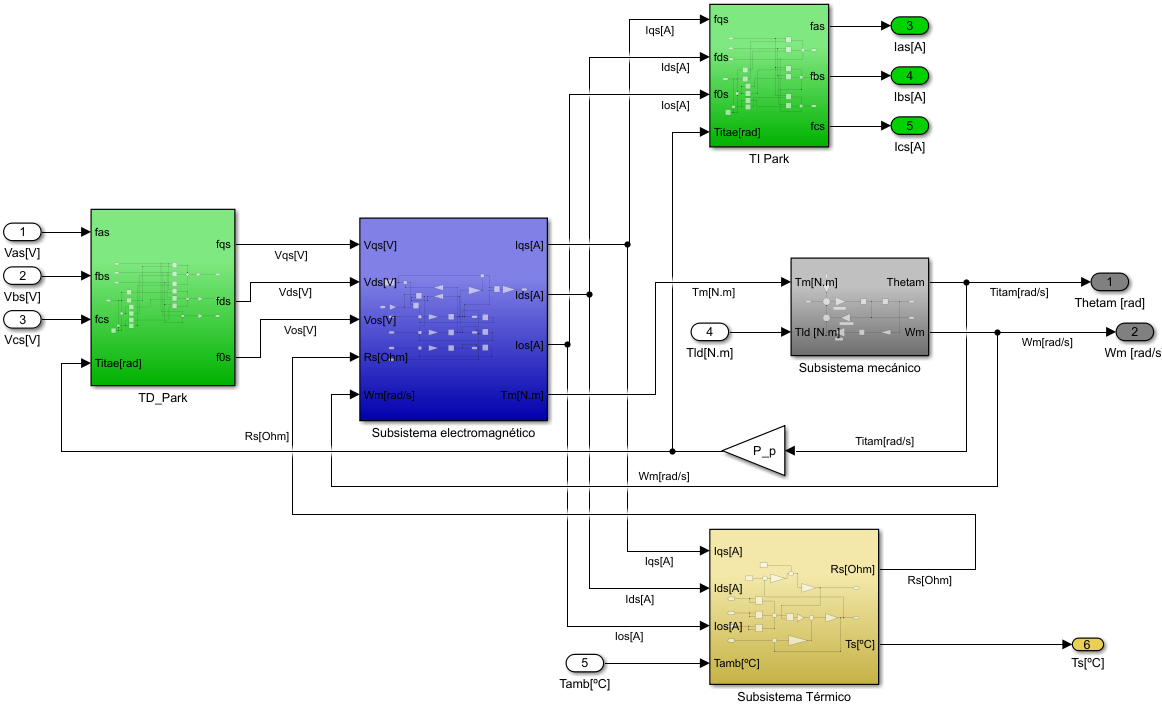
\includegraphics[width=0.85\textwidth]{Imagenes/Diagrama_Global_NoLineal.png}
    \caption{Diagrama de bloques del modelo global no lineal.}
    \end{figure}
\end{frame}

\begin{frame}{Sensores de Realimentación}\footnotesize
\textbf{Sensores de retroalimentación}
El sistema cuenta con los siguientes dispositivos físicos y sus canales de medición y acondicionamiento:
\begin{itemize}
\item 1 sensor de posición angular (codificador incremental o ``encoder'') montado en el eje de motor, asumiendo proceso de ``homing'' y decodificación idealizados $\rightarrow$ variable medida: $\theta_m(t)$, posición angular absoluta ``rectificada'' (al girar más de una revolución); tal que $\theta_l(t) = \frac{1}{r}\theta_m(t)$ y ajuste $\theta_m = 0$ (Origen o ``Home'') para $\theta_l = 0$.
\item 3 sensores de corriente instantánea de fase, montados en salida trifásica del inversor hacia bornes del estator $\rightarrow$ variables medidas: $i_{as}(t), i_{bs}(t), i_{cs}(t)$.
\item 1 sensor de temperatura (ej. RTD) en bobinado de estator $\rightarrow$ variable medida: $T^\circ_s(t)$, para monitoreo de calentamiento y estimación de resistencia de estator $R_s\left(T^\circ_s(t)\right)$.
\end{itemize}
\end{frame}


%% Modelo Global Linealizado (LPV)
%% Modelo Global Linealizado (LPV)
\begin{frame}{Modelo Global Linealizado (LPV)}\footnotesize
El problema se divide en 2 partes, un espacio de operación global No Lineal (cuasi-estacionario) y un modelo dinámico LPV (pequeñas variaciones locales), que es función de parámetros variables según el punto de operación. El sistema dinámico no-lineal se puede representar como:

\begin{equation}
\left\{
\begin{aligned}
    \dot{x}(t) &= f(x(t),u(t)); && x(t_0) = x_0, \\ 
    y(t) &= C \cdot x(t)
\end{aligned}
\right.
\label{eq:linealizacion_sistemas}
\end{equation}

Teniendo en cuenta que para una variable genérica: $z(t) = Z_0(t) + \Delta z(t)$:
\begin{equation}
\left\{
\begin{aligned}
    \dot{x}(t) &= \dot{X}_0(t) + \Delta \dot{x}(t) = f(X_0(t) + \Delta x(t), U_0(t) + \Delta u(t)), \\
    X_0(0) + \Delta x(0) &= x_0, \quad \Longrightarrow \quad X_0(0) \equiv x_0, \quad \Delta x(0) \equiv 0, \\
    Y_0(t) + \Delta y(t) &= C(X_0(t) + \Delta x(t)), \quad \Longrightarrow \quad 
    \begin{aligned}[t]
    &Y_0(t) = C X_0(t), \\
    &\Delta y(t) = C \Delta x(t).
    \end{aligned}
\end{aligned}
\right.
\end{equation}
\end{frame}

\begin{frame}{Modelo Global Linealizado (LPV)} \scriptsize
En los sistemas no lineales los puntos de equilibrio son todos aquellos en donde la variación de energía se ha disipado completamente (equilibrio dinámico). Es decir, los puntos de equilibrio son todos aquellos en donde las derivadas de las variables de estado son nulas.

\begin{equation*}
\text{Equilibrios:} \quad \dot{x}(t) = 0 = f(x(t),u(t))
\end{equation*}

A todos los pares valores de $x(t)$ e $u(t)$ que satisfacen la igualdad se lo denomina puntos de operación $(X_0,U_0)$. Los puntos de operación pueden ser constantes $\{X_0,U_0\}$ o presentar variaciones relativamente lentas en el tiempo (cuasi-estacionarios) $\{X_0(t),U_0(t)\}$.

Realizamos una expansión en serie de Taylor truncada a 1° orden (despreciando términos orden superior):
\begin{equation}
f(X_0(t) + \Delta x(t), U_0(t) + \Delta u(t)) \approx f(X_0(t),U_0(t)) + \left.\frac{\partial f}{\partial x}\right|_0 (t) \cdot \Delta x(t) + \left.\frac{\partial f}{\partial u}\right|_0 (t) \cdot \Delta u(t)
\end{equation}

Si sustituimos esta última expresión en la (Ec.~\ref{eq:linealizacion_sistemas}), vemos la división del problema en dos partes anteriormente mencionada:
\end{frame}

\begin{frame}{Modelo Global Linealizado (LPV)}\tiny
1. Una parte no lineal, que representa el espacio de operación global NL (cuasi-estacionario):
  \begin{equation}
  \dot{X}_0(t) = f(X_0(t),U_0(t)) \approx 0/ete; \quad X_0(0) = x_0
  \label{Ec.25}
  \end{equation}

Que en nuestro sistema en particular esta formado por el siguiente sistema de ecuaciones:

\begin{equation}
\left\{
\begin{aligned}
\frac{d\theta_{mO}}{dt}(t) &= \omega_{mO}(t) = cte \\
\frac{d\omega_{mO}}{dt}(t) &= \frac{1}{J_{eq}}\left[-b_{eq}\omega_{mO}(t) + \frac{3}{2}P_p[\lambda_m' + (L_d - L_q)i^r_{dsO}(t)]i^r_{qsO}(t) - g \cdot k_l \sin\Bigg(\frac{\theta_{mO}}{r}\Bigg) - \frac{1}{r} T_{ld}(t)\right] = 0 \\
\frac{di^r_{qsO}}{dt}(t) &= \frac{1}{L_q}\left[v^r_{qsO}(t) - R_s(T^\circ_{sO}(t))i^r_{qsO}(t) - (\lambda_m' + L_di^r_{dsO}(t))P_p\omega_{mO}(t)\right] = 0 \\
\frac{di^r_{dsO}}{dt}(t) &= \frac{1}{L_d}\left[v^r_{dsO}(t) - R_s(T^\circ_{sO}(t))i^r_{dsO}(t) + L_qi^r_{qsO}(t)P_p\omega_{mO}(t)\right] = 0 \\
\frac{di^r_{0sO}}{dt}(t) &= \frac{1}{L_{ls}}(v^r_{0sO}(t) - R_s(T^\circ_{sO}(t))i^r_{0sO}(t)) = 0 \\
\frac{dT^\circ_{sO}}{dt}(t) &= \frac{1}{C_{ts}}\left[\frac{3}{2}R_s(t)(i^r_{qsO}(t)^2 + i^r_{dsO}(t)^2 + 2i^r_{0sO}(t)^2) - \frac{1}{R_{ts-amb}}(T^\circ_{sO}(t) - T^\circ_{ambO}(t))\right] = 0 
\end{aligned}
\right.
\end{equation}
\end{frame}

\begin{frame}{Modelo Global Linealizado (LPV)}\tiny
2. Una parte lineal dinámica, que representa las pequeñas variaciones alrededor de puntos de Operación (Modelo dinámico lineal LPV):
\begin{equation}
\Delta\dot{x}(t) = \underbrace{\left.\frac{\partial f}{\partial x}\right|_0}_{A_o}(t)\cdot\Delta x(t) + \underbrace{\left.\frac{\partial f}{\partial u}\right|_0}_{B_o}(t)\cdot\Delta u(t); \quad \Delta x(0) = 0
\label{Ec.30}
\end{equation}

\begin{equation}
\left\{
\begin{aligned}
\Delta\dot{\theta}_m(t) &= \Delta\omega_m(t) \\
\Delta\dot{\omega}_m(t) &= \frac{1}{J_{eq}}\left[\frac{3}{2} P_p\{[\lambda_m' + (L_d - L_q)\cdot i^r_{dsO}]\cdot\Delta i^r_{qs}(t) + (L_d - L_q)\cdot i^r_{qsO}\cdot\Delta i^r_{ds}(t)\} - b_{eq}\cdot\Delta\omega_m(t)\right. \\
&\quad \left. -\frac{g\cdot k_l}{r^2} \cdot cos(\frac{\theta_{mO}}{r})\cdot\Delta\theta_m(t) - \frac{\Delta T_{ld}(t)}{r}\right] \\
\Delta\dot{i}^r_{qs}(t) &= \frac{1}{L_q}\left[\Delta v^r_{qs}(t) - R_{sO}\cdot\Delta i^r_{qs}(t) - R_{s, \text{REF}}\alpha_\text{cu}\Delta T^\circ_s(t)\cdot i^r_{qsO} - \{\lambda_m' + L_d\cdot i^r_{dsO}\} P_p\cdot\Delta\omega_m(t)\right. \\
&\quad \left. - L_d P_p\omega_{mO}\cdot\Delta i^r_{ds}(t)\right] \\
\Delta\dot{i}^r_{ds}(t) &= \frac{1}{L_d}\left[\Delta v^r_{ds}(t) - R_{sO}\cdot\Delta i^r_{ds}(t) - R_{s, \text{REF}}\alpha_\text{cu}\Delta T^\circ_s(t)\cdot i^r_{dsO} + L_q\cdot i^r_{qsO}\cdot P_p\cdot\Delta\omega_m(t)\right. \\
&\quad \left. + L_q\cdot P_p\cdot\omega_{mO}\cdot\Delta i^r_{qs}(t)\right] \\
\Delta\dot{i}^r_{0s}(t) &= \frac{1}{L_{ls}}\left[\Delta v^r_{0s}(t) - R_{sO}\cdot\Delta i^r_{0s}(t) - R_{s, \text{REF}}\alpha_\text{cu}\Delta T^\circ_s(t)\cdot i^r_{0sO}\right] \\
\Delta\dot{T}_s(t) &= \frac{1}{C_{ts}}\left[\frac{3}{2}\cdot R_{sO}\cdot(2\cdot i^r_{qsO}\cdot\Delta i^r_{qs}(t) + 2\cdot i^r_{dsO}\cdot\Delta i^r_{ds}(t) + 4\cdot i_{0sO}\cdot\Delta i_{0s}(t))\right. \\
&\quad + \left. \frac{3\alpha_{cu}R_{sREF}}{2}(i^r_{qsO}(t)^2 + i^r_{dsO}(t)^2 + 2i^r_{0sO}(t)^2)\cdot\Delta T_s(t) - \frac{1}{R_{ts-amb}}(\Delta T_s(t) - \Delta T_{amb}(t))\right]
\end{aligned}
\right.
\label{eq:SistemaGlobalLPV}
\end{equation}
\end{frame}


\begin{frame}{Modelo Global Linealizado (LPV)}\footnotesize
Donde:
\[
R_{sO} = R_{s, \text{REF}} \cdot \Big( 1 + \alpha_\text{cu} \cdot (T_{sO}^\circ - T_{s, \text{REF}}) \Big),
\]

La matriz de estado se define de la siguiente manera:

\begin{figure}[h]
\centering
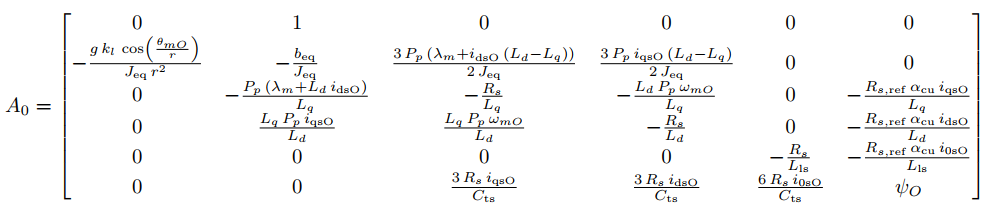
\includegraphics[width=0.95\textwidth]{Imagenes/MatrizAo.png}
\end{figure}

 Donde: 
\[
\psi_O = -\frac{\frac{1}{R_{\mathrm{ts},\mathrm{amb}}} - \frac{3\,R_{s,\mathrm{ref}}\,\alpha_{\mathrm{cu}}\,\left(2\,i_{\mathrm{0sO}}^2 + i_{\mathrm{dsO}}^2 + i_{\mathrm{qsO}}^2\right)}{2}}{C_{\mathrm{ts}}},
\]
\end{frame}

\begin{frame}{Modelo Global Linealizado (LPV)}\scriptsize
Las matrices de entradas de manipulación y perturbación para el modelo LPV son:

\begin{center}
\begin{minipage}{0.45\textwidth}
\[
B_o^c = 
\begin{bmatrix}
0 & 0 & 0 \\
0 & 0 & 0 \\
\frac{1}{L_q} & 0 & 0 \\
0 & \frac{1}{L_d} & 0 \\
0 & 0 & \frac{1}{L_{\mathrm{ls}}} \\
0 & 0 & 0
\end{bmatrix}
\]
\end{minipage}
\hfill
\begin{minipage}{0.45\textwidth}
\[
B_o^d = 
\begin{bmatrix}
0 & 0 \\
\frac{1}{J_{\mathrm{eq}} r} & 0 \\
0 & 0 \\
0 & 0 \\
0 & 0 \\
0 & \frac{1}{C_{\mathrm{ts}} R_{\mathrm{ts},\mathrm{amb}}}
\end{bmatrix}
\]
\end{minipage}
\end{center}

Finalmente, el modelo dinámico global LPV en forma matricial resulta:

\begin{equation}
\begin{bmatrix}
\Delta \dot{\theta}_m(t) \\
\Delta \dot{\omega}_m(t) \\
\Delta \dot{i}_{qs}^r(t) \\
\Delta \dot{i}_{ds}^r(t) \\
\Delta \dot{i}_{0s}(t) \\
\Delta \dot{T}_s(t)
\end{bmatrix}
=
A_o \cdot
\begin{bmatrix}
\Delta \theta_m(t) \\
\Delta \omega_m(t) \\
\Delta i_{qs}^r(t) \\
\Delta i_{ds}^r(t) \\
\Delta i_{0s}(t) \\
\Delta T_s(t)
\end{bmatrix}
+
B_o^c \cdot
\begin{bmatrix}
\Delta v_{qs}^r(t) \\
\Delta v_{ds}^r(t) \\
\Delta v_{0s}(t)
\end{bmatrix}
+
B_o^d \cdot
\begin{bmatrix}
\Delta T_{ld}(t) \\
\Delta T_{amb}(t)
\end{bmatrix}.
\end{equation}
\end{frame}
%% Modelo Simplificado lineal invariante (LTI)
\begin{frame}{Modelo Simplificado Lineal Invariante (LTI)}\footnotesize
En esta sección se obtendrá el modelo simplificado lineal invariante (LTI) equivalente, para ello se tendrán en cuenta las siguientes consideraciones:
\begin{itemize}
    
    \item Se aplica la estrategia de ``Control Vectorial con campo orientado'' que consiste en desacoplar los canales de flujo magnético y torque, forzando corriente nula en el eje \( d \), es decir, \( i^r_{ds}(t) = 0 \). Esto se produce mediante la aplicación de una ``Restricción o Ley de Control mínima sobre la variable manipulada virtual \( v^r_{qd0s}(t) \)'' o su equivalente por \( T \) de Park, \( v_{abcs}(t) \).

    \item Como el estator de la maquina en
    estudio esta conectado en estrella trifilar con neutro flotante y ademas el sistema es simétrico y equilibrado. Se tiene que: 
    \begin{equation}
    i_{as}(t) + i_{bs}(t) + i_{cs}(t) = 0
    \end{equation}
    Aplicando transformada directa de Park:
    \begin{equation}
    \label{eq:neutro_flotante}
    i_{0s}(t) = \frac{2}{3}\cdot\frac{1}{2}\cdot(i_{as}(t) + i_{bs}(t) + i_{cs}(t)) = 0 \therefore \frac{di_{0s}(t)}{dt} = 0 \rightarrow v_{0s}(t) = 0
    \end{equation}

    \item Se desacoplará el subsistema térmico y para ello se considerará que, debido a las variaciones despreciables de \( R_s \) en el rango de temperaturas de trabajo, la temperatura no producirá ninguna variación importante en el sistema.
\end{itemize}
\end{frame}

\begin{frame}{Modelo Simplificado Lineal Invariante (LTI)}\scriptsize
Con estas consideraciones, las ecuaciones vectoriales y matriciales de estado, y de salida del modelo LTI equivalente, quedan de la siguiente forma:

\begin{equation}
\left\{
\begin{aligned}
\frac{d\theta_m(t)}{dt} &= \omega_m(t) \\[1ex]
\frac{d\omega_m(t)}{dt} &= \frac{1}{J_{eq}}\left[\frac{3}{2}P_p\lambda'_m\cdot i^r_{qs}(t) - b_{eq}\cdot\omega_m(t) - \frac{1}{r}\cdot T_{ld}(t) - \frac{g \cdot k_l}{r}\sin(\frac{1}{r}\theta_m(t))\right] \\[1ex]
\frac{di^r_{qs}(t)}{dt} &= \frac{1}{L_q}\left[v^r_{qs}(t) - R_s\cdot i^r_{qs}(t) - \lambda'_mP_p\cdot\omega_m(t)\right] \\
\frac{d T_s(t)}{dt} &= \frac{1}{C_{ts}} \Bigg[ \frac{3}{2} R_s \cdot i_{qs}^r(t)^2 - \frac{1}{R_{ts-amb}} \big( T_s(t) - T_{amb}(t) \big) \Bigg].
\end{aligned}
\right.
\label{eq:sistema_LTI_equivalente}
\end{equation}

\[
\tiny
\left\{
\begin{aligned}
\frac{dx(t)}{dt} &= \begin{bmatrix} \dot{\theta}_m(t) \\ \dot{\omega}_m(t) \\ \dot{i}^r_{qs}(t) \end{bmatrix} = 
\begin{bmatrix} 
0 & 1 & 0 \\
0 & -\frac{b_{eq}}{J_{eq}} & \frac{3P_p\lambda'_m}{2J_{eq}} \\
0 & -\frac{P_p\lambda^r_m}{L_q} & -\frac{R_s}{L_q}
\end{bmatrix}
\begin{bmatrix} \theta_m(t) \\ \omega_m(t) \\ i^r_{qs}(t) \end{bmatrix} +
\begin{bmatrix} 0 \\ 0 \\ \frac{1}{L_q} \end{bmatrix}v^r_{qs}(t) +
\begin{bmatrix} 0 \\ -\frac{1}{rJ_{eq}} \\ 0 \end{bmatrix}T_{ld}(t) +
\begin{bmatrix} 0 \\ -\frac{k_l}{rJ_{eq}} \\ 0 \end{bmatrix}\sin(\frac{1}{r}\theta_m(t)) \\[2ex]
y(t) &= \begin{bmatrix} 1 & 0 & 0 \end{bmatrix}\cdot x(t), \quad
x(0) = \begin{bmatrix} \theta_m(0) \\ \omega_m(0) \\ i^r_{qs}(0) \end{bmatrix}
\end{aligned}
\right.
\]
\end{frame}

\begin{frame}{Modelo Simplificado Lineal Invariante (LTI)}
    En la siguiente figura se observa el diagrama de bloques desagregado escalar del sistema LTI equivalente correspondiente a la ecuación de estado (Ec.~\ref{eq:sistema_LTI_equivalente})
    \begin{figure}[h]
    \centering
    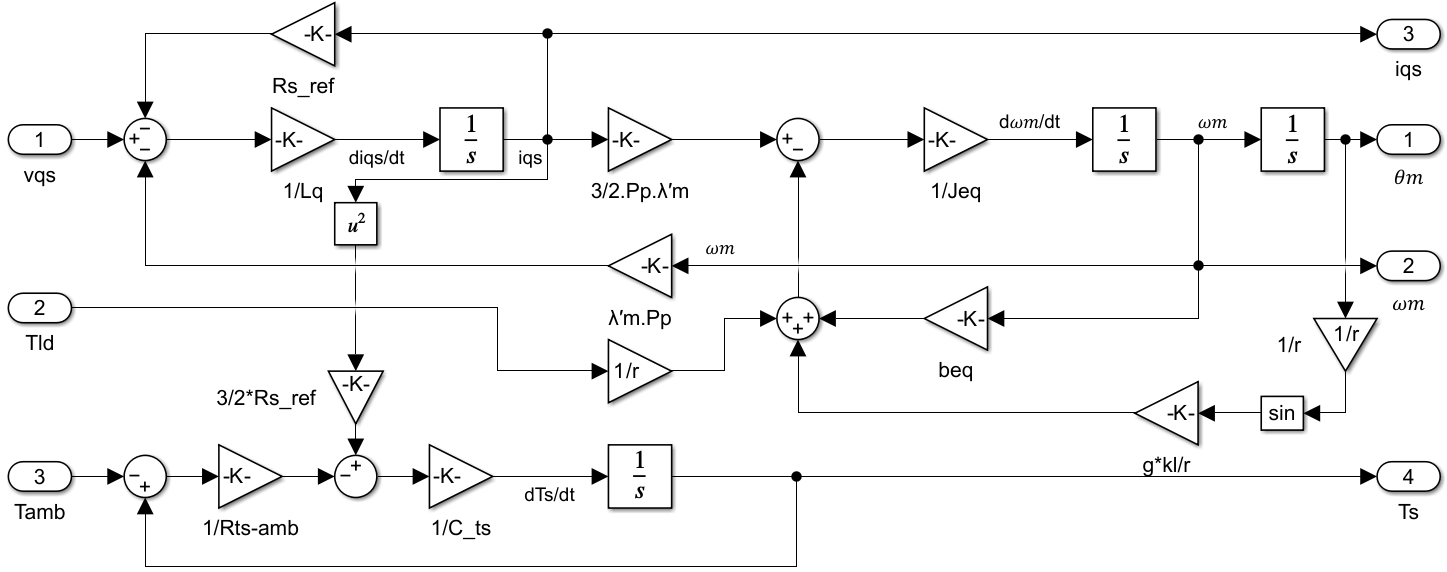
\includegraphics[width=0.85\textwidth]{Imagenes/SistEqLTI.png}
    \caption{Diagrama de bloques de estado modelo LTI equivalente.}
    \end{figure}
\end{frame}

\begin{frame}{Ley de Control Mínima}\footnotesize
Para cumplir la especificación ``$i^r_{ds}(t) = 0$'', asumiendo estado inicial de \(i^r_{ds}\) nulo ``$i^r_{ds}(0) = 0$'' (desacoplamiento de canales de flujo magnético y torque) la restricción o ley de control mínima que es necesario aplicar sobre la variable manipulada virtual ``$v^r_{ds}$'' se obtiene de una de las ecuaciones de estado del sistema:
\begin{equation}
i_{ds}(t) =  0 \rightarrow \frac{di_{ds}(t)}{dt} = 0
\end{equation}
\begin{equation}
\cancel{\frac{d i_{ds}^r(t)}{dt}} = \frac{1}{L_d} \Big( v_{ds}^r(t) - \cancel{R_s(t) i_{ds}^r(t)} + L_q i_{qs}^r(t) P_p \cdot \omega_m(t) \Big)
\label{eq:ExpresionIds}
\end{equation}
\begin{equation}
\frac{1}{L_d}\left[v^r_{ds}(t) + L_qi^r_{qs}(t)P_p\omega_m(t)\right] = 0 \rightarrow v^r_{ds}(t) = -L_q\cdot i^r_{qs}(t)\cdot P_p\cdot\omega_m(t)
\end{equation}

La variable que se manipula en el sistema es la tensión, pero expresada en el sistema coordenado ``abc'', de modo que será necesario aplicar la transformación inversa de Park para regresar al sistema original.
\end{frame}

\begin{frame}{Ley de Control Mínima}\tiny
Aplicamos la transformación inversa a las tensiones de entrada, para aplicar el control que nos permita lograr las restricciones propuestas anteriormente:

\begin{equation}
\begin{bmatrix}
v_{as}(t) \\
v_{bs}(t) \\
v_{cs}(t)
\end{bmatrix} = 
\begin{bmatrix}
\cos \theta_r(t) & \sin \theta_r(t) & 1 \\
\cos(\theta_r(t)-\frac{2\pi}{3}) & \sin(\theta_r(t)-\frac{2\pi}{3}) & 1 \\
\cos(\theta_r(t)+\frac{2\pi}{3}) & \sin(\theta_r(t)+\frac{2\pi}{3}) & 1
\end{bmatrix}
\begin{bmatrix}
v^r_{qs}(t) \\
v^r_{ds}(t) \\
v^r_{0s}(t)
\end{bmatrix}
\label{Ec.37}
\end{equation}

\begin{equation}
\begin{cases}
v_{as}(t) &= \cos \theta_r(t)\cdot v^r_{qs}(t) + \sin \theta_r(t)\cdot v^r_{ds}(t) + v^r_{0s}(t) \\
v_{bs}(t) &= \cos\left(\theta_r(t)-\frac{2\pi}{3}\right)\cdot v^r_{qs}(t) + \sin\left(\theta_r(t)-\frac{2\pi}{3}\right)\cdot v^r_{ds}(t) + v^r_{0s}(t) \\
v_{cs}(t) &= \cos\left(\theta_r(t)+\frac{2\pi}{3}\right)\cdot v^r_{qs}(t) + \sin\left(\theta_r(t)+\frac{2\pi}{3}\right)\cdot v^r_{ds}(t) + v^r_{0s}(t)
\end{cases}
\end{equation}

Sustituimos los valores de $v^r_{qs}(t)$ y $v^r_{ds}(t)$ ya conocidos, y teniendo la Ec.~\ref{eq:neutro_flotante}:

\begin{equation}
\begin{cases}
v_{as}(t) = \cos \theta_r(t)\cdot v^r_{qs}(t) - \sin \theta_r(t)\cdot L_q\cdot i^r_{qs}(t)\cdot P_p\cdot\omega_m(t) \\
v_{bs}(t) = \cos\left(\theta_r(t)-\frac{2\pi}{3}\right)\cdot v^r_{qs}(t) - \sin\left(\theta_r(t)-\frac{2\pi}{3}\right)\cdot L_q\cdot i^r_{qs}(t)\cdot P_p\cdot\omega_m(t) \\
v_{cs}(t) = \cos\left(\theta_r(t)+\frac{2\pi}{3}\right)\cdot v^r_{qs}(t) - \sin\left(\theta_r(t)+\frac{2\pi}{3}\right)\cdot L_q\cdot i^r_{qs}(t)\cdot P_p\cdot\omega_m(t)
\end{cases}
\end{equation}
De forma similar para los valores de corriente se tendrá:
\begin{equation}
\begin{cases}
i_{as}(t) = \cos \theta_r(t)\cdot i^r_{qs}(t)  \\
i_{bs}(t) = \cos\left(\theta_r(t)-\frac{2\pi}{3}\right)\cdot i^r_{qs}(t) \\
i_{cs}(t) = \cos\left(\theta_r(t)+\frac{2\pi}{3}\right)\cdot i^r_{qs}(t)
\end{cases}
\end{equation}
De esta forma determinamos la Restricción o Ley de Control mínima que es necesario aplicar para lograr el desacoplamiento de canales de flujo magnético y torque.
\end{frame}

\begin{frame}{Ley de Control Mínima}
    \begin{figure}[h]
    \centering
    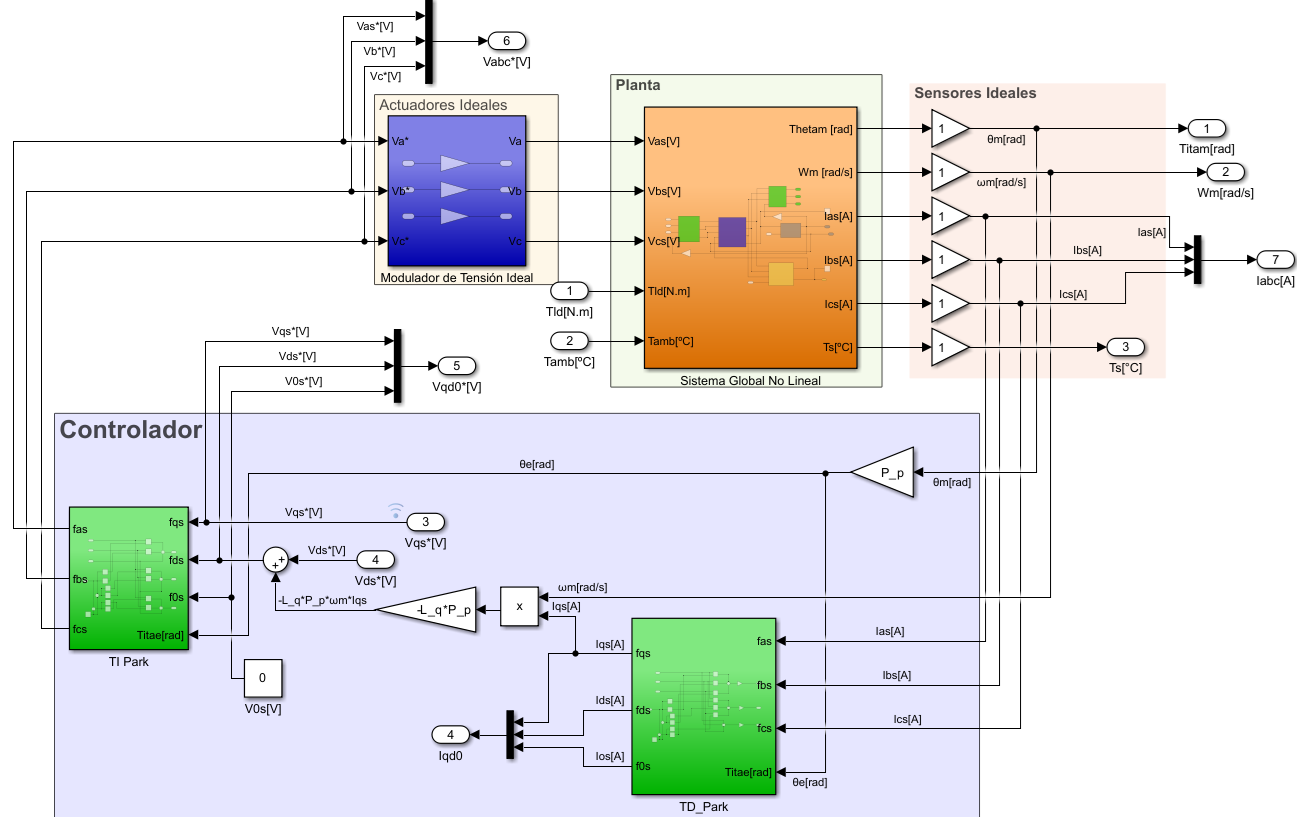
\includegraphics[width=0.85\textwidth]{Imagenes/BloquesLinealizacionRealimentacionNoLineal.png}
    \caption{Diagrama de bloques del sistema linealizado por realimentación parcial de estados mediante un controlador
    parcial externo.}
    \end{figure}
\end{frame}

\begin{frame}{Modelo de la Dinámica Residual}\scriptsize
    Con el propósito de modelar la dinámica residual equivalente para $i^r_{ds}(t)$ en el caso general donde no se cumpla la hipótesis asumida para el estado inicial de $i^r_{ds}(t)$ se aplica la ley de control mínima encontrada para $v^r_{ds}(t)$ de la ecuación de estado.
    \begin{equation}
    \frac{d i_{ds}^r(t)}{dt} = \frac{1}{L_d} \Big( \cancel{v_{ds}^r(t)} - R_s(t) i_{ds}^r(t) + \cancel{L_q i_{qs}^r(t) P_p \cdot \omega_m(t)} \Big)
    \end{equation}
    \begin{equation}
    L_d \cdot\frac{di^r_{ds}}{dt}(t) + R_s(t)\cdot i^r_{ds}(t) = 0 \quad \rightarrow \quad \frac{di^r_{ds}}{dt}(t) = \frac{1}{L_d}\left[-R_s(t)\cdot i^r_{ds}(t)\right]
    \end{equation}
    Al resolver esta ecuación encontramos que:
    \begin{equation}
    i^r_{ds}(t) = i^r_{ds}(0)\cdot e^{-\frac{R_s(t)}{L_d}\cdot t}
    \end{equation}
    Analizando esta expresión vemos que la corriente decae exponencialmente. Es así que el error de la dinámica residual es debido a un valor inicial de la corriente distinta de cero ``$i^r_{ds}(0) \neq 0$'', lo cual genera un acoplamiento en el eje q y produce un comportamiento no lineal del sistema que desaparecerá al cabo del tiempo, afectando la respuesta natural del sistema pero no así en régimen forzado y es por dicha razón que se puede despreciarlo.
    \begin{equation}
    v^r_{qs}(t) = L_q\cdot \frac{di^r_{qs}}{dt}(t) + R_s(t)\cdot i^r_{ds}(t) + \lambda'_m\cdot P_p\cdot\omega_m(t) + \boldsymbol{L_d\cdot P_p\cdot\omega_m(t)\cdot i^r_{ds}(t)}
    \end{equation}
\end{frame}

\begin{frame}{Modelo de la Dinámica Residual}\footnotesize
    Si incorporamos esta dinámica residual, despreciando el acoplamiento residual NL con el eje q, al modelo LTI equivalente:
\begin{equation}
\scriptsize
\left\{
\begin{aligned}
\frac{d\theta_m}{dt}(t) &= \omega_m(t) \\[1ex]
\frac{d\omega_m}{dt}(t) &= \frac{1}{J_{eq}}\left[\frac{3}{2}P_p\lambda^r_mi^r_{qs}(t) - b_{eq}\omega_m(t) - \frac{1}{r}T_{ld}(t) - \frac{g \cdot k_l}{r} \sin\Bigg(\frac{\theta_m(t)}{r}\Bigg)\right] \\[1ex]
\frac{di^r_{qs}}{dt}(t) &= \frac{1}{L_q}\left[v^r_{qs}(t) - R_si^r_{qs}(t) - \lambda^r_mP_p\omega_m(t)\right] \\[1ex]
\frac{di^r_{ds}}{dt}(t) &= -\frac{1}{L_d}R_s\cdot i^r_{ds}(t) \\[1ex]
\frac{d T_s(t)}{dt} &= \frac{1}{C_{ts}} \Bigg[ \frac{3}{2} R_s \cdot \big(i_{qs}^r(t)^2+i_{ds}^r(t)^2\big) - \frac{1}{R_{ts-amb}} \big( T_s(t) - T_{amb}(t) \big) \Bigg]
\end{aligned}
\right.
\label{eq:sistema_LTI_aumentado}
\end{equation}
\end{frame}

\begin{frame}{Ley de Control Complementaria Mínima}
    \scriptsize
    Se puede implementar una Restricción o Ley de Control complementaria mínima en el eje q para eliminar completamente este acoplamiento residual NL aún en régimen natural
    y obtener un modelo equivalente completamente lineal, independiente del estado inicial de
    \(i^r_{ds}(t)\).
    
    \begin{equation}
    \tiny
    v^r_{qs}(t) + \cancel{\boldsymbol{L_d\cdot P_p\cdot\omega_m(t)\cdot i^r_{ds}(t)}} = L_q\cdot \frac{di^r_{qs}}{dt}(t) + R_s(t)\cdot i^r_{qs}(t) + \lambda'_m\cdot P_p\cdot\omega_m(t) + \cancel{\boldsymbol{L_d\cdot P_p\cdot\omega_m(t)\cdot i^r_{ds}(t)}}
    \end{equation}
    \begin{figure}[h]
    \centering
    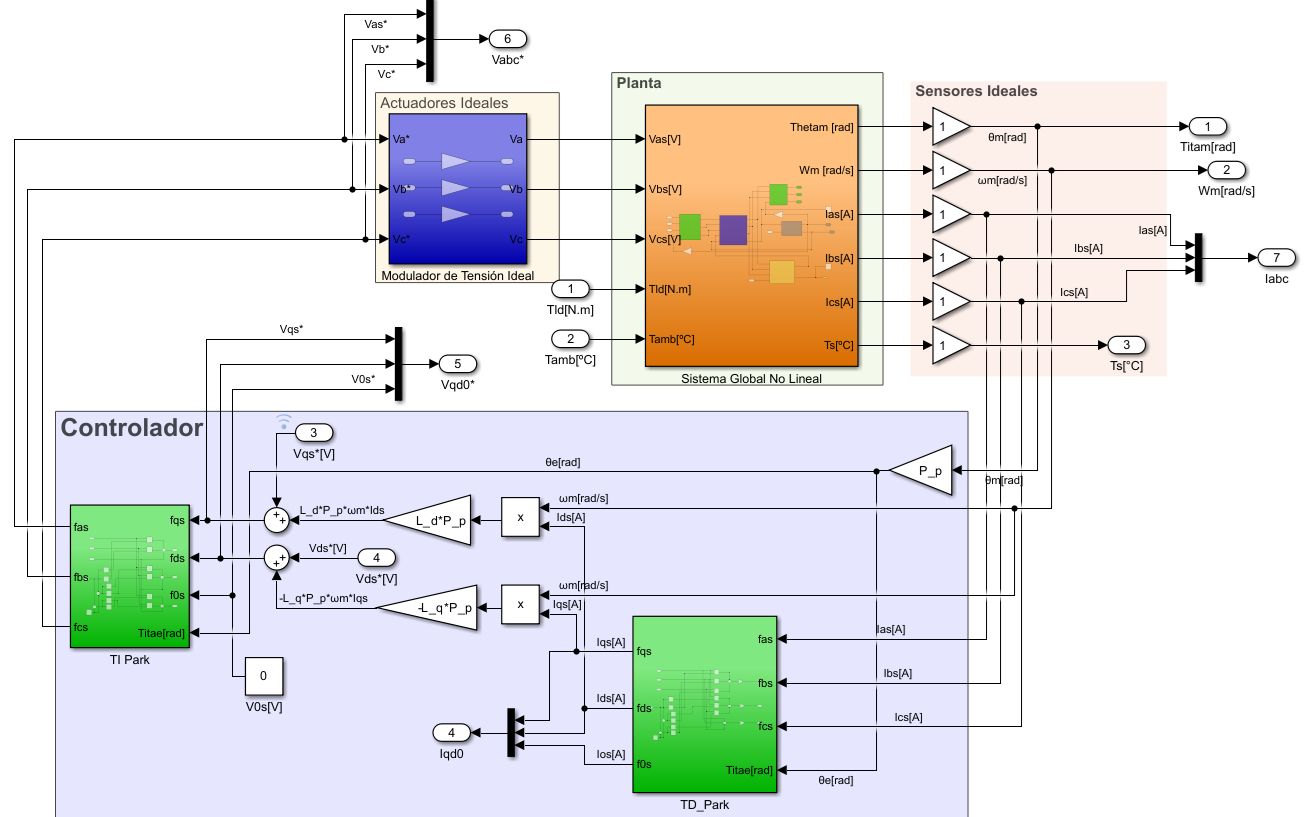
\includegraphics[width=0.75\textwidth]{Imagenes/BloquesLinealizacionRealimentacionNoLinealDesacoplo.png}
    \caption{Implementación de Ley de Control complementaria mínima en el eje q mediante el controlador parcial.}
    \end{figure}
\end{frame}

\begin{frame}{Modelo Simplificado Lineal Invariante (LTI)}
    \scriptsize
    La diferencia entre este modelo con el modelo Global No Lineal con las leyes de control para desacoplar los canales de flujo magnético y torque, es que en el modelo LTI aumentado no se considera la variación de la resistencia con la temperatura \(T^\circ_s(t)\).

\begin{figure}[H]
    \centering
    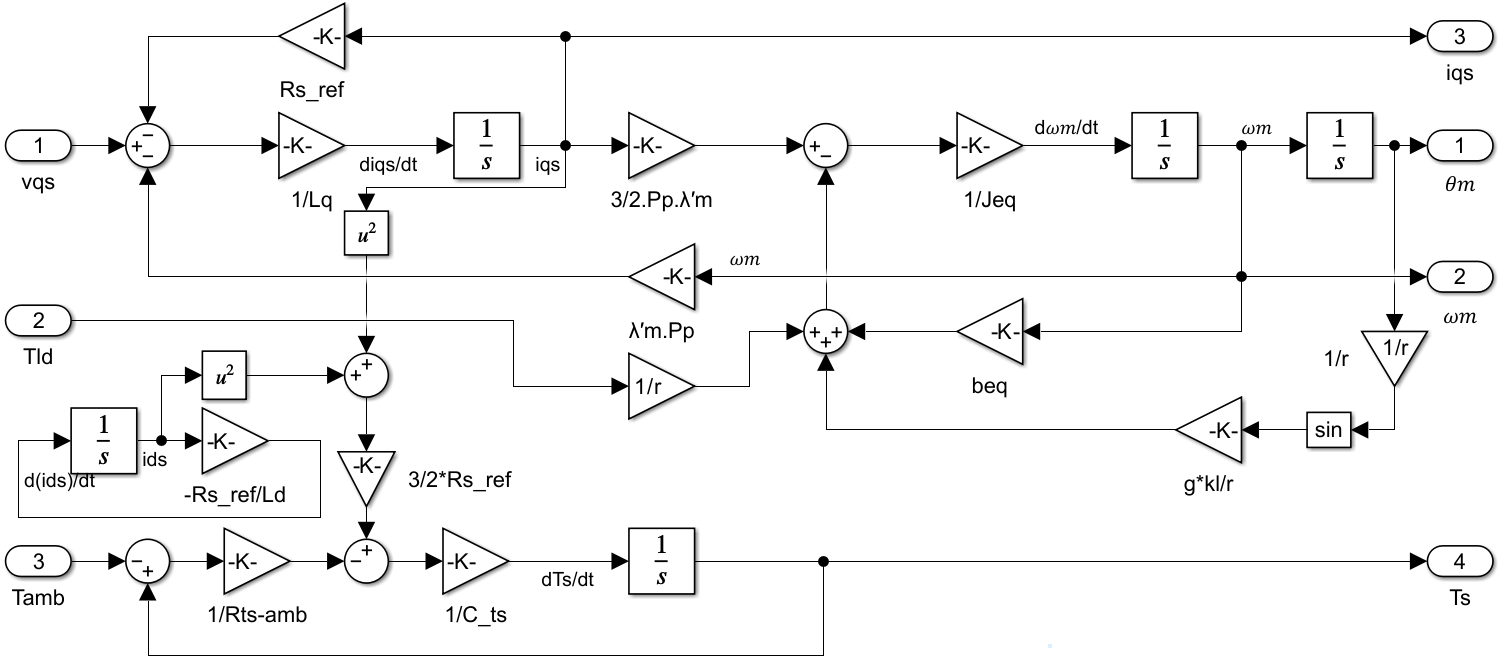
\includegraphics[width=0.9\textwidth]{Imagenes/SistEqLTI_aumentado.png}
    \caption{Diagrama de bloques desagregado del sistema LTI aumentado.}
    \label{fig:diagrama_sistema_LTI_aumentado}
\end{figure}
\end{frame}

\begin{frame}{Modelo Dinámico LTI Equivalente Aumentado vs Modelo Dinámico Global LPV}\footnotesize
    \textbf{Aspectos principales}
    \begin{itemize}
        \item El modelo dinámico global LPV para el caso general ``\(i^r_{ds} \neq 0\)'' representa mejor al sistema real, ya que se tiene un espacio con mayor cantidad de puntos de operación.
        \item El modelo dinámico LTI equivalente aumentado es un caso particular del modelo dinámico global LPV, en donde \(i^r_{ds} = 0\). Realizar esta simplificación implica reducir el espacio de puntos de operación, pero presenta como ventaja un modelo con mucha mayor simplicidad en comparación con el modelo dinámico global LPV.
        \item El modelo dinámico global LPV considera la variación de \(R_{s}(T^\circ_{s}(t))\), en cambio el modelo dinámico LTI equivalente aumentado toma la simplificación de considerar \(R_{s}\) constante.
    \end{itemize}
    Podemos ver la similitud entre el modelo dinámico global LPV presentado en la (Ec.~\ref{eq:SistemaGlobalLPV}), considerando \(I_{dsr_o} \equiv 0\) y el sistema LTI mostrado en la (Ec.~\ref{eq:sistema_LTI_aumentado}).
\end{frame}

\begin{frame}{Modelo Dinámico LTI Equivalente Aumentado vs Modelo Dinámico Global LPV}\footnotesize
\textbf{Análisis del comportamiento del sistema frente a variaciones en ``\(i^r_{ds}\)''}

Por otro lado, como la corriente directa está orientada en el mismo sentido que el campo
principal de la máquina, su variación tiene un efecto en el torque electromagnético $T_{m}$ y la velocidad de rotación
Al primer análisis lo realizamos con respecto al par electromagnético, recordando Ec.~\ref{eq:SubsistemaElectromagnetico}:
 \begin{equation*}
     T_m(t) = \frac{3}{2} P_p [\lambda'^r_m + (L_d - L_q) i_{ds}^r(t)] i_{qs}^r(t).
 \end{equation*}

\begin{itemize}
    \item \textbf{Corriente directa nula (\(i^r_{ds}(t) = 0\))}: Sólo existe flujo concatenado por imanes permanentes (\(\lambda'^r_m\)).
    
    \item \textbf{Reforzamiento de Campo (\(i^r_{ds}(t) > 0\))}: Sabemos que para motores de polos salientes \(L_d > L_q\) , entonces cuando \(i^r_{ds}(t)\) toma valores más positivos, el campo
    magnético principal se refuerza aumentando el torque en el motor. 
    
    \item \textbf{Debilitamiento de Campo (\(i^r_{ds}(t) < 0\))}: En este caso, según la Ec.~\ref{eq:SubsistemaElectromagnetico}, el torque disminuye debido al término \((L_d - L_q)i^r_{ds}(t)\).
\end{itemize}
\end{frame}

\begin{frame}{\small Modelo Dinámico LTI Equivalente Aumentado vs Modelo Dinámico Global LPV}\scriptsize
Ahora analizando lo que pasa con la velocidad, recordando (Ec.~\ref{eq:ExpresionIds}):
 \begin{equation*}
     \frac{d i_{ds}^r(t)}{dt} = \frac{1}{L_d} \Big( v_{ds}^r(t) - R_s(t) i_{ds}^r(t) + L_q i_{qs}^r(t) P_p \cdot \omega_m(t) \Big) = 0 \rightarrow \omega_m(t) = \frac{-v^r_{ds}(t) + R_s(t).i^r_{ds}(t)}{L_q.i^r_{qs}(t).P_p}
 \end{equation*}

\begin{itemize}
    \item \textbf{Corriente directa nula (\(i^r_{ds}(t) = 0\))}: El flujo concatenado está afectado únicamente por los imanes permanentes, y el motor alcanza un estado de equilibrio dinámico entre el par motor y su velocidad.
    
    \item \textbf{Reforzamiento de Campo (\(i^r_{ds}(t) > 0\))}: La velocidad del motor disminuye (ya que el término positivo $R_s(t).i^r_{ds}(t)$ se opone al término negativo $-v^r_{ds}(t)$). 
    
    \item \textbf{Debilitamiento de Campo (\(i^r_{ds}(t) < 0\))}: En este caso, pasa lo contrario al caso anterior con respecto al término $R_s(t).i^r_{ds}(t)$, y la velocidad del motor aumenta.
\end{itemize}
\end{frame}

\begin{frame}{Variación de Parámetros en Modelo LPV}\scriptsize
    \textbf{Migración de Propiedades ante Variación de \(i_{ds}\)}
    A continuación, se presentan los resultados obtenidos para diferentes valores de \( i_{ds} \). Cada fila muestra 6 autovalores del sistema para un valor dado de \( i_{ds} \):

\begin{table}[H]
    \tiny
    \centering
    \label{tab:variacion_i_ds}
    \begin{tabular}{|c|c|}
        \hline
        \textbf{i\_ds [A]} & \textbf{Autovalores (6 en total)} \\
        \hline
        -1.500 & $-0.1+0.0j \quad -88.4+54.6j \quad -88.4-54.6j \quad -154.5+0.0j \quad -0.0+0.0j \quad -1275.0+0.0j$ \\
        \hline
        -1.155 & $-0.1+0.0j \quad -88.4+85.0j \quad -88.4-85.0j \quad -154.5+0.0j \quad -0.0+0.0j \quad -1275.0+0.0j$ \\
        \hline
        -0.810 & $-0.1+0.0j \quad -88.4+107.7j \quad -88.4-107.7j \quad -154.5+0.0j \quad -0.0+0.0j \quad -1275.0+0.0j$ \\
        \hline
        -0.466 & $-0.1+0.0j \quad -88.5+127.0j \quad -88.5-127.0j \quad -154.5+0.0j \quad -0.0+0.0j \quad -1275.0+0.0j$ \\
        \hline
        -0.121 & $-0.1+0.0j \quad -88.5+144.3j \quad -88.5-144.3j \quad -154.5+0.0j \quad -0.0+0.0j \quad -1275.0+0.0j$ \\
        \hline
         0.224 & $-0.0+0.0j \quad -88.5+160.1j \quad -88.5-160.1j \quad -154.5+0.0j \quad -0.0+0.0j \quad -1275.0+0.0j$ \\
        \hline
    \end{tabular}
    \caption{Variación de los 6 autovalores ante cambios en \( i_{ds} \)}
\end{table}
\end{frame}

\begin{frame}{Variación de Parámetros en Modelo LPV}
    \begin{figure}[H]
    \centering
    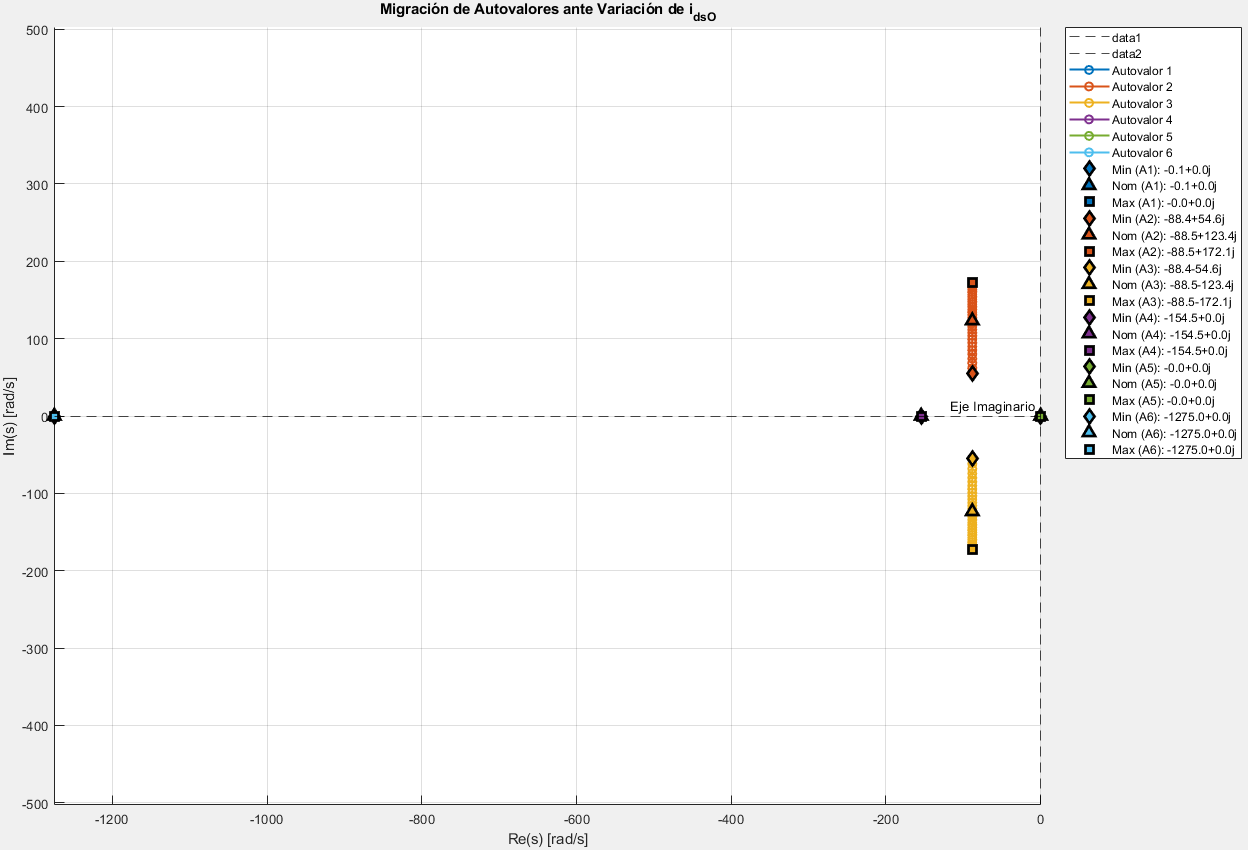
\includegraphics[width=0.85\textwidth]{Imagenes/MigracionLPV_1.png}
    \label{fig:migracion_polos_i_ds}
    \end{figure}
\end{frame}

\begin{frame}{Variación de Parámetros en Modelo LPV}
    \begin{figure}[H]
    \centering
    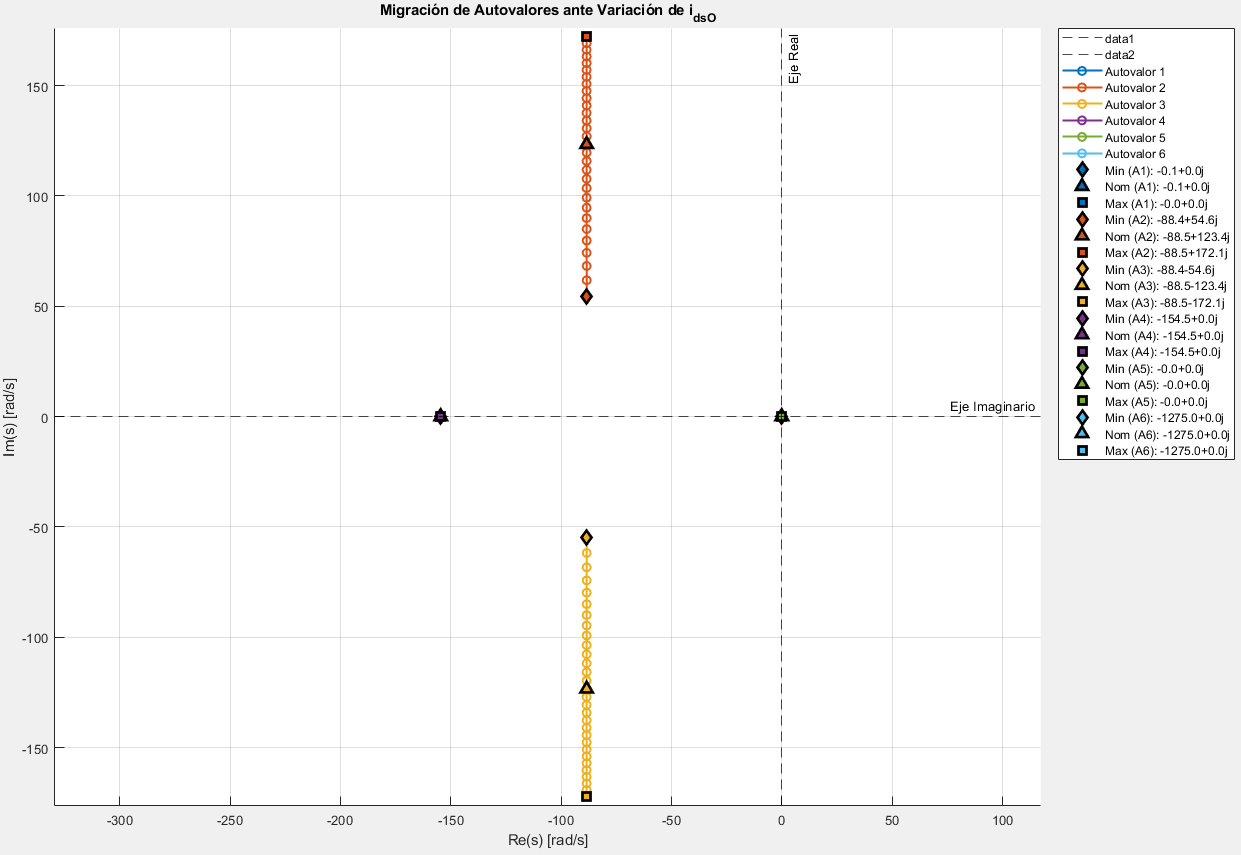
\includegraphics[width=0.85\textwidth]{Imagenes/MigracionLPV_2.png}
    \label{fig:migracion_polos_i_ds}
    \end{figure}
\end{frame}

\begin{frame}{\small Funciones de Transferencia para el Modelo LTI Equivalente Aumentado}\small
    Para obtener las funciones de transferencia desde las entradas \( v_{qsr}(t) \) y \( T_l(t) \) hacia la salida \( \theta_m(t) \) para el modelo LTI equivalente aumentado, partimos del sistema completo y aplicamos las siguientes consideraciones:
    
    \begin{itemize}
    \item \textbf{Subsistema Térmico Desacoplado}: Consideramos \( R_s(t) = R_s \) constante.
    \item \textbf{Control Vectorial Orientado a Campo}: Se asume \( i_{ds}^r(t) = 0 \).
    \item \textbf{Condiciones Iniciales Nulas}: Todas las condiciones iniciales se consideran nulas para la aplicación de la transformada de Laplace.
    \end{itemize}
\end{frame}

\begin{frame}{\small Funciones de Transferencia para el Modelo LTI Equivalente Aumentado}\scriptsize
    \textbf{Definición de \( T_l(t) \)}

Definimos la variable \( T_l(t) \) como:

\[
T_l(t) = T_{ld}(t) + g \cdot k_l \sin\left(\frac{\theta_m(t)}{r}\right)
\]


\textbf{Sistema Reducido con \( T_l(t) \)}


\[
\left\{
\begin{aligned}
\frac{d\theta_m}{dt}(t) &= \omega_m(t) \\[1ex]
\frac{d\omega_m}{dt}(t) &= \frac{1}{J_{eq}} \left[ \frac{3}{2} P_p \lambda'^r_m i^r_{qs}(t) - b_{eq} \omega_m(t) - \frac{1}{r}\cdot T_l(t) \right] \\[1ex]
\frac{di^r_{qs}}{dt}(t) &= \frac{1}{L_q} \left[ v^r_{qs}(t) - R_s i^r_{qs}(t) - \lambda'^r_m P_p \omega_m(t) \right]
\end{aligned}
\right.
\]


\textbf{Aplicación de la Transformada de Laplace}

\[
\left\{
\begin{aligned}
s\Theta_m(s) &= \Omega_m(s) \\[1ex]
s\Omega_m(s) &= \frac{1}{J_{eq}} \left[ \frac{3}{2} P_p \lambda'^r_m I^r_{qs}(s) - b_{eq} \Omega_m(s) - T_l(s) \right] \\[1ex]
sI^r_{qs}(s) &= \frac{1}{L_q} \left[ V^r_{qs}(s) - R_s I^r_{qs}(s) - \lambda'^r_m P_p \Omega_m(s) \right]
\end{aligned}
\right.
\]
\end{frame}

\begin{frame}{\small Funciones de Transferencia para el Modelo LTI Equivalente Aumentado}\scriptsize
    \textbf{Resolución del Sistema}


\[
I^r_{qs}(s) = \frac{V^r_{qs}(s) - \lambda'^r_m P_p \Omega_m(s)}{L_q s + R_s}
\]


\[
s\Omega_m(s) = \frac{1}{J_{eq}} \left[ \frac{3}{2} P_p \lambda'^r_m \cdot \frac{V^r_{qs}(s) - \lambda'^r_m P_p \Omega_m(s)}{L_q s + R_s} - b_{eq} \Omega_m(s) - T_l(s) \right]
\]


\[
\Omega_m(s) = \frac{\frac{3}{2} P_p \lambda'^r_m V^r_{qs}(s) - (L_q s + R_s) T_l(s)}{J_{eq} L_q s^2 + (J_{eq} R_s + b_{eq} L_q) s + \left(b_{eq} R_s + \frac{3}{2} P_p^2 (\lambda'^r_m)^2\right)}
\]


\[
\Theta_m(s) = \frac{\Omega_m(s)}{s} = \frac{\frac{3}{2} P_p \lambda'^r_m V^r_{qs}(s) - (L_q s + R_s) T_l(s)}{s \left( J_{eq} L_q s^2 + (J_{eq} R_s + b_{eq} L_q) s + \left(b_{eq} R_s + \frac{3}{2} P_p^2 (\lambda'^r_m)^2 \right) \right)}
\]

\textbf{Funciones de Transferencia}

\[
\Theta_m(s) = G_{V_{qs}}(s) \cdot V^r_{qs}(s) + G_{T_l}(s) \cdot T_l(s)
\]

Donde:
\begin{equation}
G_{V_{qs}}(s) = \frac{\frac{3}{2} P_p \lambda'^r_m}{J_{eq} L_q s^3 + (J_{eq} R_s + b_{eq} L_q) s^2 + \left(b_{eq} R_s + \frac{3}{2} P_p^2 (\lambda'^r_m)^2\right) s}
\end{equation}
\begin{equation}
G_{T_l}(s) = \frac{-(L_q s + R_s)}{J_{eq} L_q s^3 + (J_{eq} R_s + b_{eq} L_q) s^2 + \left(b_{eq} R_s + \frac{3}{2} P_p^2 (\lambda'^r_m)^2\right) s}
\end{equation}
\end{frame}

\begin{frame}{\small Funciones de Transferencia para el Modelo LTI Equivalente Aumentado} \footnotesize
\textbf{Estados Internos no Reflejados en las Funciones de Transferencia}

En el modelo LTI equivalente aumentado completo, existen cinco estados internos:

\begin{itemize}
    \item \( \theta_m(t) \): Posición angular del motor
    \item \( \omega_m(t) \): Velocidad angular del motor
    \item \( i_{qs}^r(t) \): Corriente del eje \( q \)
    \item \( i_{ds}^r(t) \): Corriente del eje \( d \)
    \item \( T_s(t) \): Temperatura del estator
\end{itemize}

Sin embargo, en las funciones de transferencia obtenidas \( G_{V_{qs}}(s) \) y \( G_{T_l}(s) \), sólo se reflejan tres de estos estados (\( \theta_m(t) \), \( \omega_m(t) \) e \( i_{qs}^r(t) \)). Los estados \( i_{ds}^r(t) \) y \( T_s(t) \) no aparecen debido a:

\begin{itemize}
    \item \( i_{ds}^r(t) \): Se mantiene en cero por el control vectorial de campo orientado, y su dinámica está desacoplada del sistema principal.
    \item \( T_s(t) \): Al desacoplar el subsistema térmico y considerar \( R_s \) constante, la temperatura del estator no afecta directamente al modelo electromagnético.
\end{itemize}
\end{frame}

\begin{frame}{Análisis de Estabilidad a lazo abierto}\scriptsize
    \textbf{Polinomio característico:}
    \[
    J_{eq} L_q s^3 + (J_{eq} R_s + b_{eq} L_q) s^2 + \left(b_{eq} R_s + \frac{3}{2} P_p^2 (\lambda'^r_m)^2\right) s = 0
    \]
    \textbf{Polos:}
    \[
    \left\{
    \begin{aligned}
    s_1 &= 0 \\
    s_{2,3} &= -\frac{L_{q}\,b_{\mathrm{eq}} + J_{\mathrm{eq}}\,R_{s}\pm\sqrt{{J_{\mathrm{eq}}}^2\,{R_{s}}^2 - 6\,J_{\mathrm{eq}}\,L_{q}\,{P_{p}}^2\,{\lambda_{r,m}}^2 - 2\,J_{\mathrm{eq}}\,L_{q}\,R_{s}\,b_{\mathrm{eq}} + {L_{q}}^2\,{b_{\mathrm{eq}}}^2}}{2\,J_{\mathrm{eq}}\,L_{q}} 
    \end{aligned}
    \right.
    \]
    
    Reemplazando los parámetros:
    \[
    \left\{
    \begin{aligned}
    s_1 &= 0 \\
    s_2 &= -88.5 + 149.9j \ \text{rad/s} \\
    s_3 &= -88.5 - 149.9j \ \text{rad/s}
    \end{aligned}
    \right.
    \]
    \textbf{Ceros:}
    \begin{itemize}
    \item \( G_{V_{qs}}(s) \) no presenta ceros finitos ya que su numerador es constante.
    \item \( G_{T_l}(s) \) presenta un cero en:
    \[
    z = -\frac{R_s}{L_q} = -175.862 \ \text{rad/s}
    \]
\end{itemize}
\end{frame}

\begin{frame}{Análisis de Estabilidad a Lazo Abierto}\scriptsize
    \textbf{Frecuencia Natural y Amortiguamiento:}
    \[
    \omega_n = \sqrt{30312} \approx 174.1 \ \text{rad/s} \quad \zeta = \frac{176.97}{2 \cdot 174.1} \approx 0.508 
    \]
    \begin{figure}[H]
    \centering
    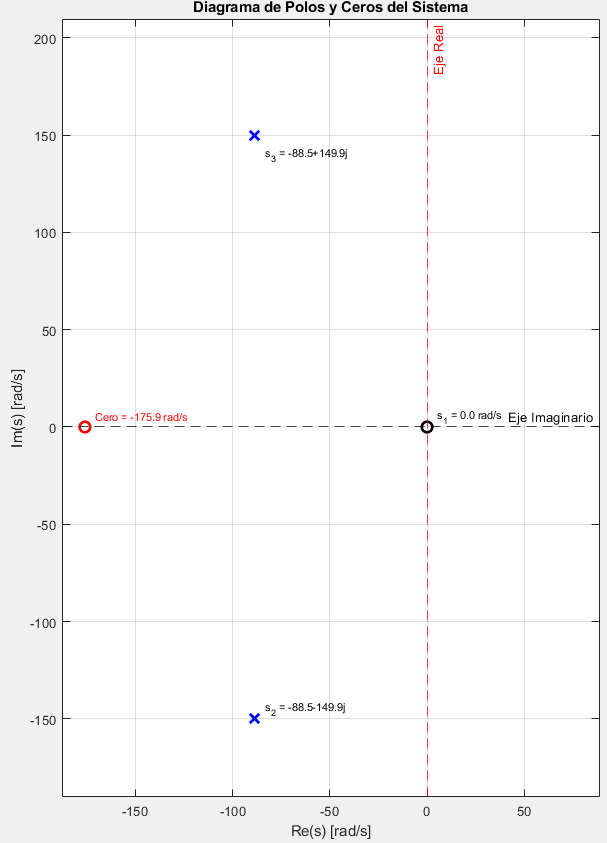
\includegraphics[width=0.4\textwidth]{Imagenes/mapa_polos_ceros.png}
    \caption{Mapa de polos y ceros a lazo abierto}
    \label{fig:polos_ceros}
    \end{figure}
\end{frame}

\begin{frame}{Migración de Propiedades ante Variación de Rs} \scriptsize
Para comprender cómo la resistencia del estator (\( R_s \)) afecta la dinámica del sistema, se realizó un análisis de variación de \( R_s \) dentro de un rango de \([0.8 \cdot R_s^{\text{ref}}, 1.2 \cdot R_s^{\text{ref}}]\), donde \( R_s^{\text{ref}} \) es el valor nominal de la resistencia. Este análisis permite observar cómo cambian las posiciones de los polos y ceros en el plano \( s \), lo que influye directamente en la estabilidad y el comportamiento transitorio del sistema.

\textbf{Resultados de la Variación de Rs}

A continuación, se presentan los resultados obtenidos para diferentes valores de \( R_s \):

\begin{table}[H]
    \centering
    \label{tab:variacion_Rs}
    \begin{tabular}{|c|c|c|c|c|}
        \hline
        \textbf{Rs [ohms]} & \textbf{Polos} & \textbf{Cero} & \textbf{\(\omega_n\) [rad/s]} & \textbf{\(\zeta\)} \\
        \hline
        0.816 & $s_{2,3} = -70.9 \pm 158.9j$ & -140.69 & 174.0 & 0.41 \\
        \hline
        0.849 & $s_{2,3} = -73.8 \pm 157.6j$ & -146.43 & 174.0 & 0.42 \\
        \hline
        0.883 & $s_{2,3} = -76.6 \pm 156.2j$ & -152.17 & 174.0 & 0.44 \\
        \hline
        0.916 & $s_{2,3} = -79.5 \pm 154.8j$ & -157.92 & 174.0 & 0.46 \\
        \hline
        0.949 & $s_{2,3} = -82.4 \pm 153.3j$ & -163.66 & 174.1 & 0.47 \\
        \hline
        0.983 & $s_{2,3} = -85.3 \pm 151.8j$ & -169.40 & 174.1 & 0.49 \\
        \hline
        1.016 & $s_{2,3} = -88.1 \pm 150.2j$ & -175.14 & 174.1 & 0.51 \\
        \hline
        1.049 & $s_{2,3} = -91.0 \pm 148.4j$ & -180.89 & 174.1 & 0.52 \\
        \hline
        1.082 & $s_{2,3} = -93.9 \pm 146.7j$ & -186.63 & 174.1 & 0.54 \\
        \hline
        1.116 & $s_{2,3} = -96.7 \pm 144.8j$ & -192.37 & 174.2 & 0.56 \\
        \hline
        1.149 & $s_{2,3} = -99.6 \pm 142.9j$ & -198.11 & 174.2 & 0.57 \\
        \hline
        1.182 & $s_{2,3} = -102.5 \pm 140.9j$ & -203.86 & 174.2 & 0.59 \\
        \hline
        1.216 & $s_{2,3} = -105.4 \pm 138.7j$ & -209.60 & 174.2 & 0.60 \\
        \hline
    \end{tabular}
\end{table}
\end{frame}

\begin{frame}{Análisis de Estabilidad a Lazo Abierto}
\scriptsize
    \begin{figure}[H]
    \centering
    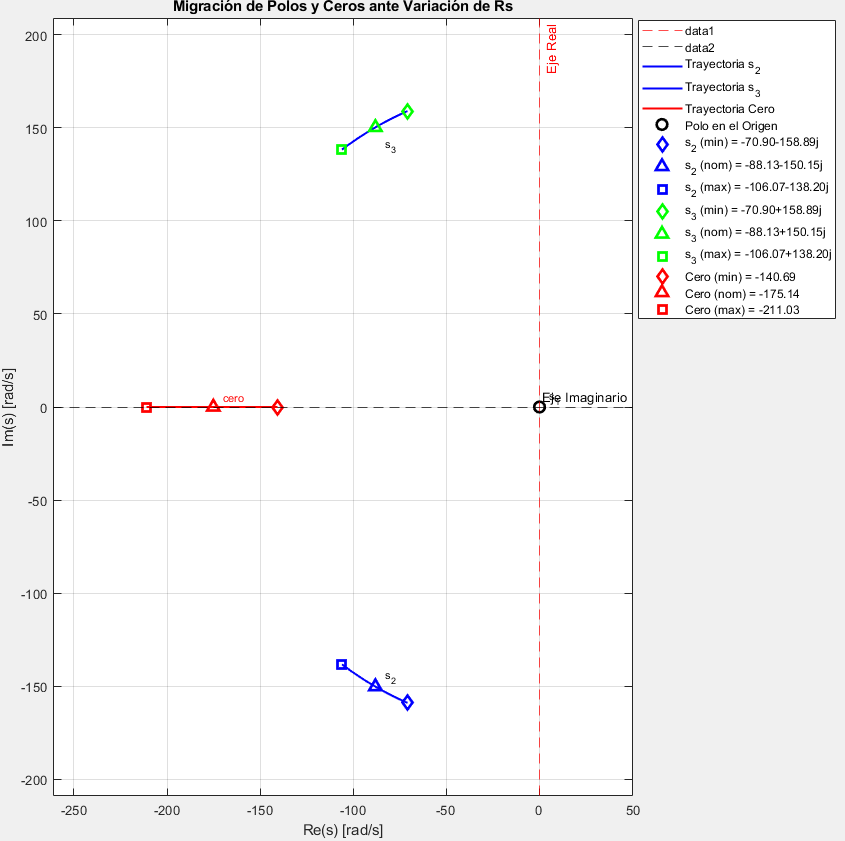
\includegraphics[width=0.6\textwidth]{Imagenes/migracion_polos_ceros.png}
    \caption{Migración de Polos y Ceros ante Variación de \( R_s \)}
    \label{fig:migracion_polos_ceros}
\end{figure}
\end{frame}

%% Observabilidad Completa de Estado
\begin{frame}{Observabilidad Completa de Estado}\scriptsize
La matriz de estado \( A \) y las matrices de salida \( C_{\theta} \) y \( C_{\omega} \) están definidas como sigue:

\[
A = \begin{bmatrix}
0 & 1 & 0 \\
0 & -\frac{b_{\text{eq}}}{J_{\text{eq}}} & \frac{3 P_{p} \lambda'_{m}}{2 J_{\text{eq}}} \\
0 & -\frac{P_{p} \lambda'_{m}}{L_q} & -\frac{R_s}{L_q}
\end{bmatrix}
\]

\[
C_{\theta} = \begin{bmatrix}
1 & 0 & 0
\end{bmatrix}, \quad
C_{\omega} = \begin{bmatrix}
0 & 1 & 0
\end{bmatrix}
\]
\textbf{Observabilidad desde la Salida Medida $\theta_m(t)$}

La matriz de observabilidad \( O_{\theta} \) se construye utilizando la matriz de estado \( A \) y la matriz de salida \( C_{\theta} \), como se define en la siguiente expresión:

\[
O_{\theta} = \begin{bmatrix}
C_{\theta} \\
C_{\theta} A \\
C_{\theta} A^2
\end{bmatrix}
\]

Donde \( C_{\theta} \) es la matriz que mide la posición \(\theta_m(t)\). La matriz resultante es:

\[
O_{\theta} = \begin{bmatrix}
1 & 0 & 0 \\
0 & 1 & 0 \\
0 & -\frac{b_{\text{eq}}}{J_{\text{eq}}} & \frac{3 P_{p} \lambda'_{m}}{2 J_{\text{eq}}}
\end{bmatrix}
\]

El rango de la matriz de observabilidad es 3, lo que indica que el sistema es completamente observable desde la salida medida \(\theta_m(t)\).
    
\end{frame}

\begin{frame}{Observabilidad Completa de Estado}\scriptsize
\textbf{Observabilidad desde la Salida Medida $\omega_m(t)$}

Para la salida medida de la velocidad angular \(\omega_m(t)\), la matriz de observabilidad \( O_{\omega} \) se construye de manera similar utilizando la matriz de salida \( C_{\omega} \):

\[
O_{\omega} = \begin{bmatrix}
C_{\omega} \\
C_{\omega} A \\
C_{\omega} A^2
\end{bmatrix}
\]

La matriz de observabilidad \( O_{\omega} \) se expresa como:

\[
O_{\omega} = \begin{bmatrix}
0 & 1 & 0 \\
0 & -\frac{b_{\text{eq}}}{J_{\text{eq}}} & \frac{3 P_{p} \lambda'_{m}}{2 J_{\text{eq}}} \\
0 & \frac{b_{\text{eq}}^2}{J_{\text{eq}}^2} - \frac{3 P_{p}^2 (\lambda'_{m})^2}{2 J_{\text{eq}} L_q} & -\frac{3 P_{p} b_{\text{eq}} \lambda'_{m}}{2 J_{\text{eq}}^2} - \frac{3 P_{p} R_s \lambda'_{m}}{2 J_{\text{eq}} L_q}
\end{bmatrix}
\]

El rango de la matriz de observabilidad es 2, lo que indica que el sistema NO es completamente observable desde la salida medida \(\omega_m(t)\). Esto se debe a que por más que se conozca la velocidad del sistema, no es posible obtener la posición del mismo sin conocer la condición inicial de posición. Caso contrario a lo que sucede cuando se conoce la posición del sistema, ya que si se la deriva, se puede llegar a conocer la velocidad del mismo.
\end{frame}

%% Controlabilidad Completa de Estado
\begin{frame}{Controlabilidad Completa de Estado}\scriptsize
La matriz de estado \( A \) y la matriz de entrada \( B \) están definidas como sigue:

\[
A = \begin{bmatrix}
0 & 1 & 0 \\
0 & -\frac{b_{\text{eq}}}{J_{\text{eq}}} & \frac{3 P_{p} \lambda'_{m}}{2 J_{\text{eq}}} \\
0 & -\frac{P_{p} \lambda'_{m}}{L_q} & -\frac{R_s}{L_q}
\end{bmatrix}, \quad
B = \begin{bmatrix}
0 \\
0 \\
\frac{1}{L_q}
\end{bmatrix}
\]

A partir de las matrices de estado \( A \) y de entrada \( B \), se construye la matriz de controlabilidad \( C \), que se expresa como:

\[
C = \begin{bmatrix}
B & A B & A^2 B
\end{bmatrix}
\]

La matriz de controlabilidad \( C \) resultante es:

\[
C = \begin{bmatrix}
0 & 0 & \frac{3 P_p \lambda'_{m}}{2 J_{\text{eq}} L_q} \\
0 & \frac{3 P_p \lambda'_{m}}{2 J_{\text{eq}} L_q} & -\frac{\frac{3 P_p b_{\text{eq}} \lambda'_{m}}{2 J_{\text{eq}}^2} + \frac{3 P_p R_s \lambda'_{m}}{2 J_{\text{eq}} L_q}}{L_q} \\
\frac{1}{L_q} & -\frac{R_s}{L_q^2} & \frac{\frac{R_s^2}{L_q^2} - \frac{3 P_p^2 \lambda^{'2}_{m}}{2 J_{\text{eq}} L_q}}{L_q}
\end{bmatrix}
\]

El rango de la matriz de controlabilidad es 3, lo que indica que el sistema \textbf{es completamente controlable} desde la entrada manipulada \( v_{qsr}(t) \). Esto implica que, con esta única entrada de control, es posible controlar todos los estados del sistema.
\end{frame}

%% Simulación Dinámica
\begin{frame}{Simulación Dinámica} \scriptsize
    Respuesta del estado interno $\{\theta_m(t); \omega_m(t); i_{qs}^r(t); i_{ds}^r(t); T_s^\circ(t)\}$ (y $v_{ds}^r(t)$ forzada) a pulso de consigna de tensión de estator en eje q: $v_{qs}^r(t) = 0\,\text{V} \Rightarrow v_{qs}^r = +19.596\,V_\text{CC}$ en $t_\text{step1} = 0.1\,\text{s} \Rightarrow 0\,\text{V}$ en $t_\text{step4} = 0.7\,\text{s}$, superpuesto con doble pulso de torque de carga $T_{ld}(t) = 0 \Rightarrow (T_{ld}_\text{max} = +6.28\,\text{N.m}\, \text{en}\, t_\text{step2} = 0.3\,\text{s}) \Rightarrow (-T_{ld}_\text{max} = -6.28\,\text{N.m}\, \text{en}\, t_\text{step3} = 0.5\,\text{s}) \Rightarrow (0\,\text{N.m}\, \text{en}\, t_\text{step5} = 0.9\,\text{s})$.

    \begin{figure}[H]
    \centering
    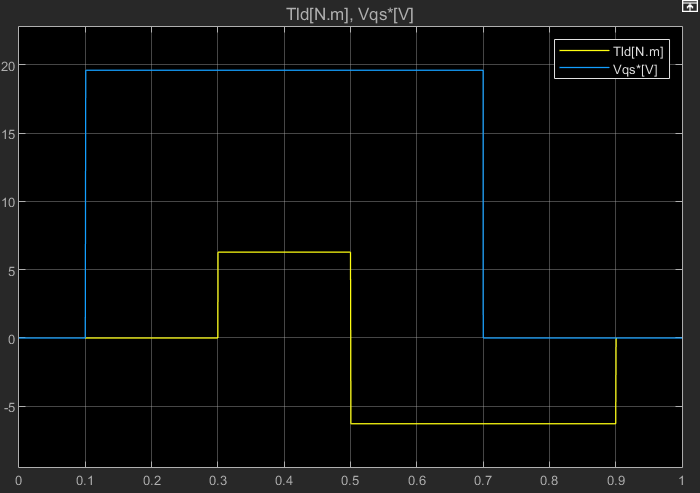
\includegraphics[width=0.6\textwidth]{Imagenes/EntradasTdVq.png}
    \caption{Consignas de Tensión \(V^{r*}_{qs}\) y Torque de carga \(T_{ld}\).}
    \label{fig:EntradasSimulacionDT}
    \end{figure}
\end{frame}

\begin{frame}{Simulación Dinámica}
    \begin{figure}[H]
    \centering
    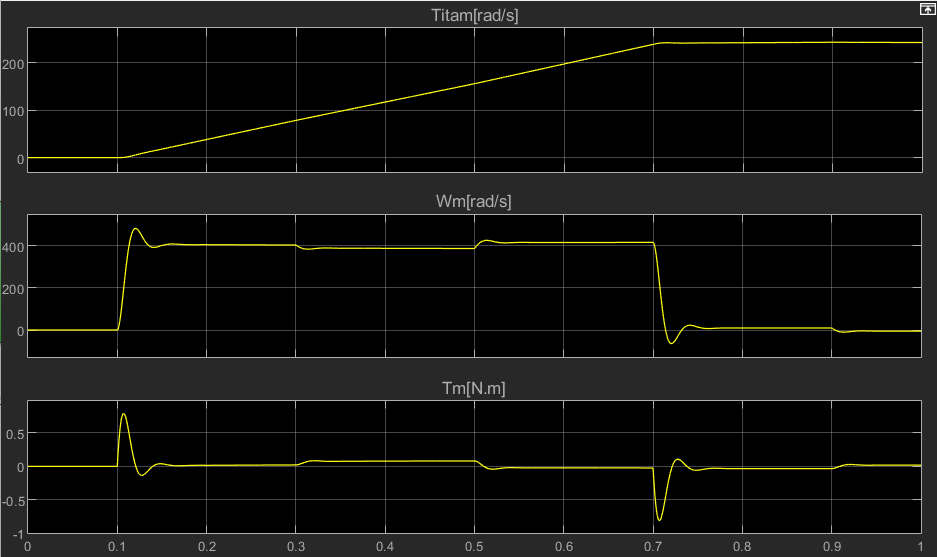
\includegraphics[width=0.85\textwidth]{Imagenes/VelPosTorqueAlineados.png}
    \caption{Curvas de posición angular, velocidad angular y torque electromagnético.}
    \label{fig:VelPosTorqueAlineados}
\end{figure}
\end{frame}

\begin{frame}{Simulación Dinámica}
    En la Figura se observa como varía la temperatura de los bobinados del estator, considerando una perturbación de la temperatura ambiente igual a 20°C.
\begin{figure}[H]
    \centering
    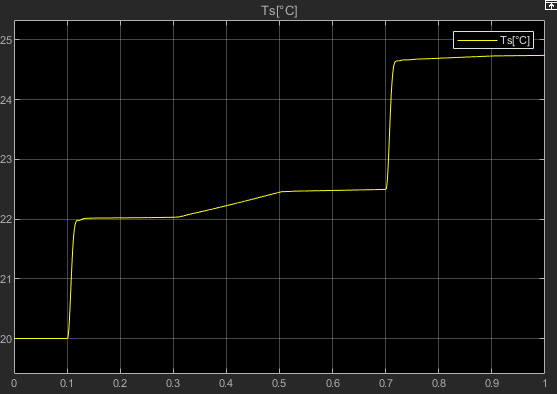
\includegraphics[width=0.55\textwidth]{Imagenes/TemperaturaEstatorDT.png}
    \caption{Temperatura de bobinados del estator.}
    \label{fig:TemperaturaEstatorDT}
\end{figure}
\end{frame}

\begin{frame}{Simulación Dinámica}\scriptsize
Los cambios en la consigna de tensión \(V^{r*}_{ds}\) se debe a la realimentación No Lineal de desacople entre los ejes q y d del controlador parcial. Esta realimentación logra que, como se observa en las gráficas, la corriente \(i^r_{ds}\) sea nula.
\begin{figure}[H]
    \centering
    \begin{tikzpicture}
        \node (image) at (0,0)
        {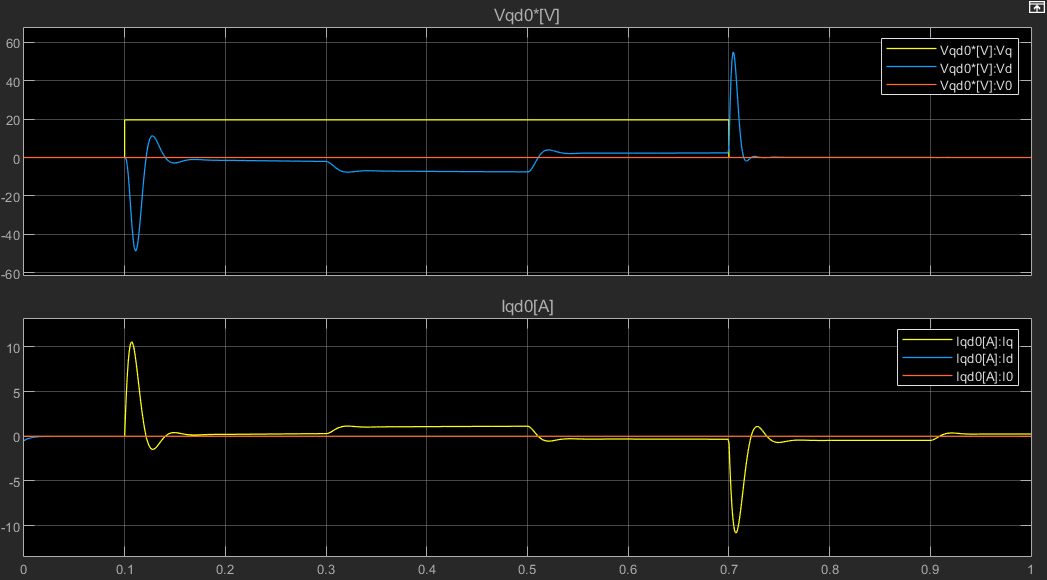
\includegraphics[width=0.9\textwidth]{Imagenes/ComparacionTensionesCorrientesVirtuales.png}};
        % Ajustar la posición del nodo a la esquina inferior derecha del primer gráfico
        \node[anchor=north east, fill=white, rounded corners, draw=black] at (5, 1) 
        {\(\mathbf{V^{r*}_{ds}(t) = -L_q \cdot i^r_{qs}(t) \cdot P_p \cdot \omega_m(t)}\)};
    \end{tikzpicture}
    \caption{Tensiones y corrientes en coordenadas virtuales.}
    \label{fig:ComparacionTensionesCorrientesVirtuales}
\end{figure}
\end{frame}

\begin{frame}{Simulación Dinámica}\scriptsize
\begin{figure}[H]
    \centering
    % Primera figura
    \begin{minipage}[t]{0.9\textwidth}
        \centering
        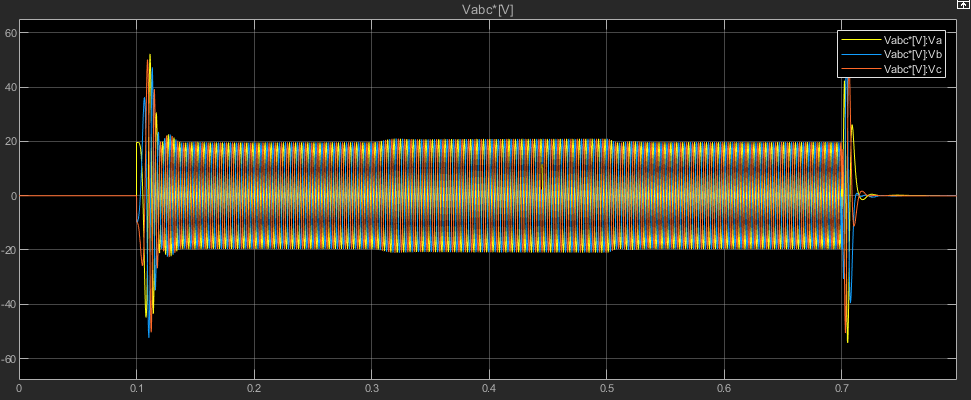
\includegraphics[width=0.7\textwidth]{Imagenes/ConsignasTensionABC.png}
        \caption{Tensiones reales abc \(V_{abcs}\).}
        \label{fig:TensionesRealesGlobalDT}
    \end{minipage}
    \begin{minipage}[t]{0.9\textwidth}
        \centering
        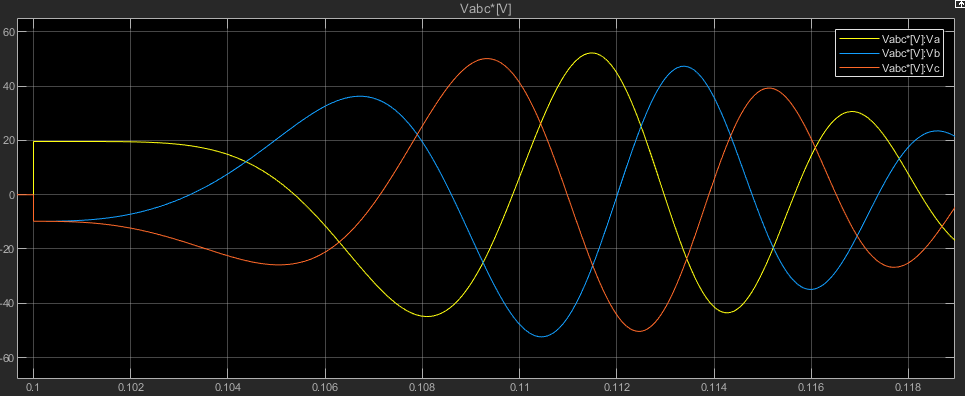
\includegraphics[width=0.7\textwidth]{Imagenes/ConsignasTensionABCacercamiento.png}
        \caption{Acercamiento a \(t = 0{.}1\,\text{s}\).}
        \label{fig:TensionesRealesAcercamientoGlobalDT}
    \end{minipage}
    \label{fig:SimulaciónTensionesCoordenadasReales}
\end{figure}
\end{frame}

\begin{frame}{Simulación Dinámica}\scriptsize
\begin{figure}[H]
    \centering
    % Primera figura
    \begin{minipage}[t]{0.9\textwidth}
        \centering
        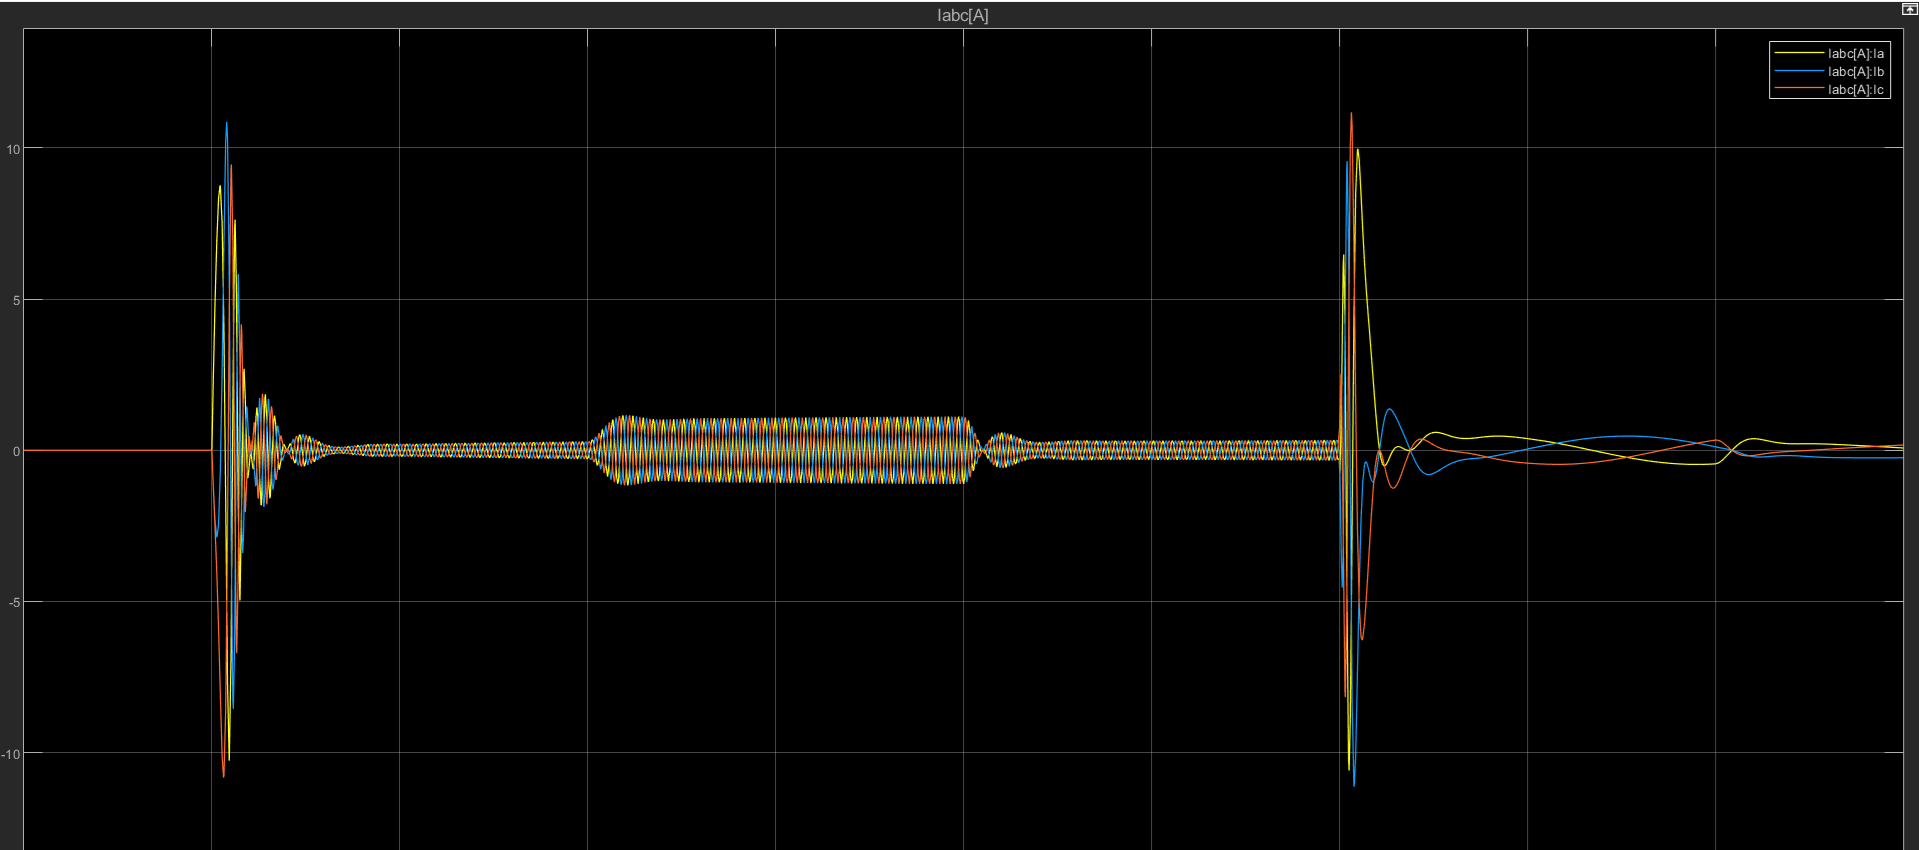
\includegraphics[width=0.6\textwidth]{Imagenes/CorrientesABCSimulacion.png}
        \caption{Corrientes reales abc \(I_{abcs}\).}
        \label{fig:CorrientesRealesGlobalDT}
    \end{minipage}
    \begin{minipage}[t]{0.9\textwidth}
        \centering
        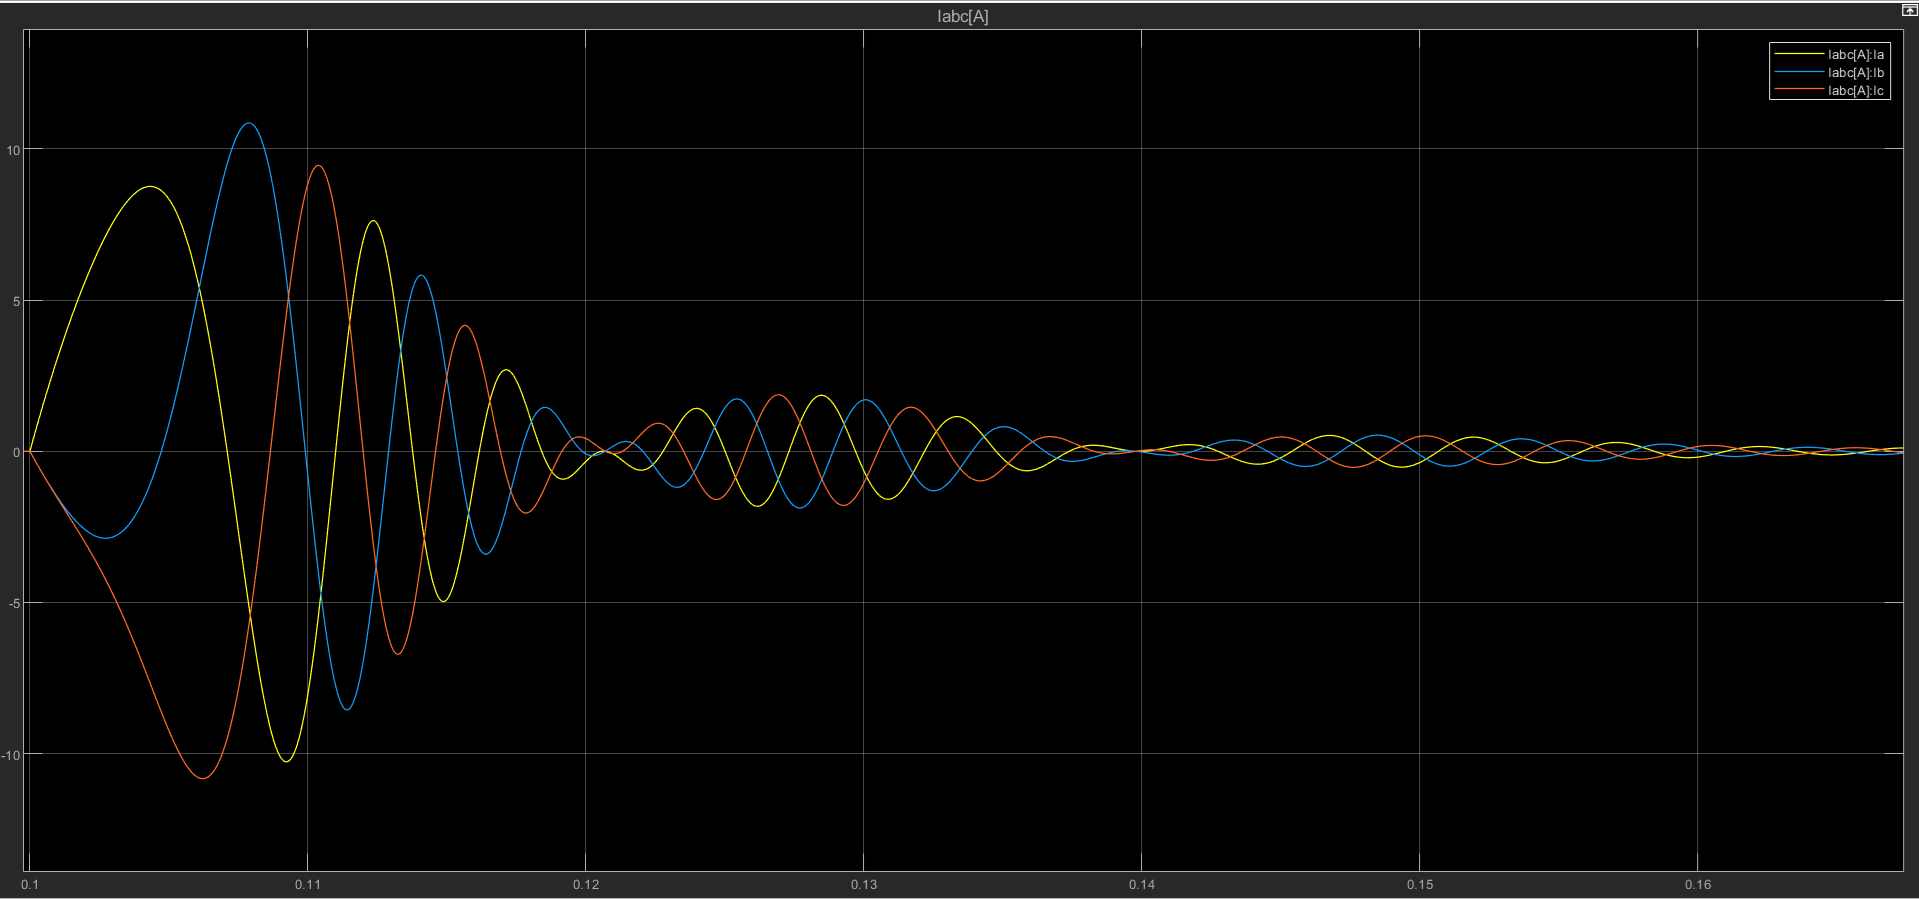
\includegraphics[width=0.6\textwidth]{Imagenes/CorrientesABCacercamientoSimulacion.png}
        \caption{Acercamiento a $t = 0{.}1\,\text{s}$.}
        \label{fig:CorrientesRealesAcercamientoGlobalDT}
    \end{minipage}
    \label{fig:SimulaciónCorrientesCoordenadasReales}
\end{figure}
\end{frame}


%% Comparación de Modelos
\begin{frame}{Comparación de Modelos NL vs LTI}\scriptsize
\begin{itemize}
\footnotesize
    \item Modelos NL vs LTI presentan respuestas similares.
    \item Desacoplamiento efectivo en ejes \( q \) y \( d \).
\end{itemize}

\begin{figure}[h]
    \centering
    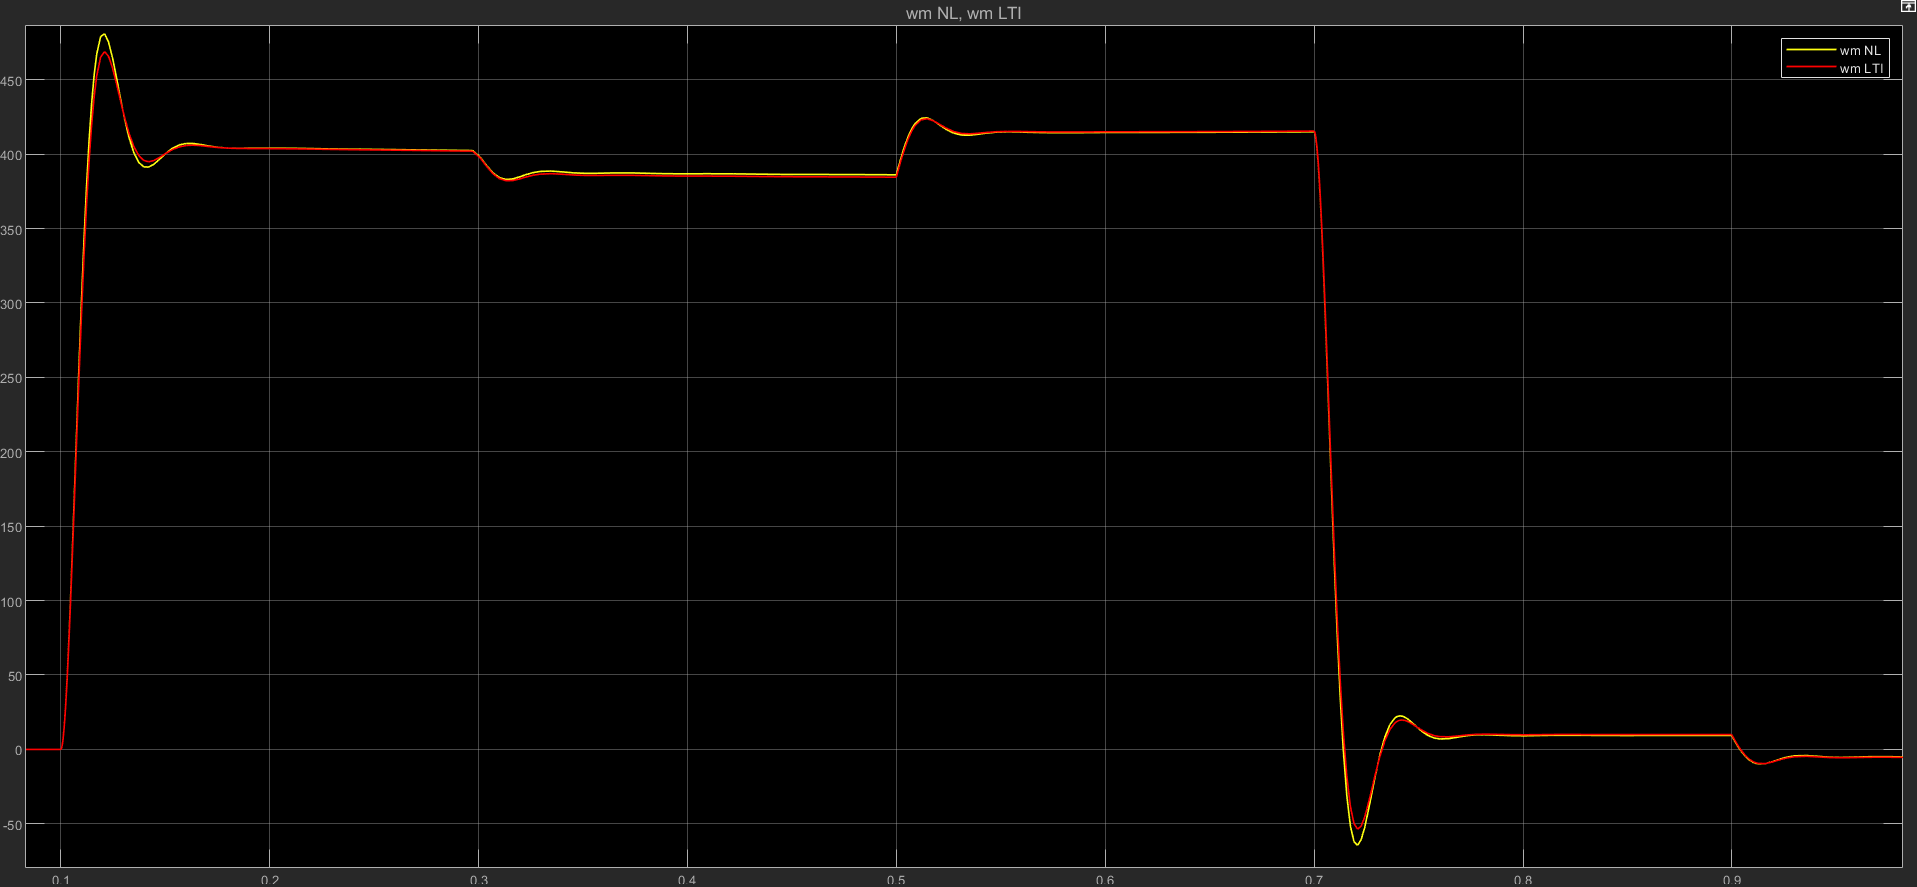
\includegraphics[width=0.9\textwidth]{Imagenes/ComparativaVelocidadAngular.png}
    \caption{Velocidad angular: NL(amarillo) vs LTI(rojo).}
\end{figure}
\end{frame}

\begin{frame}{Comparación de Modelos NL vs LTI}\scriptsize
    \begin{figure}[H]
    \centering
    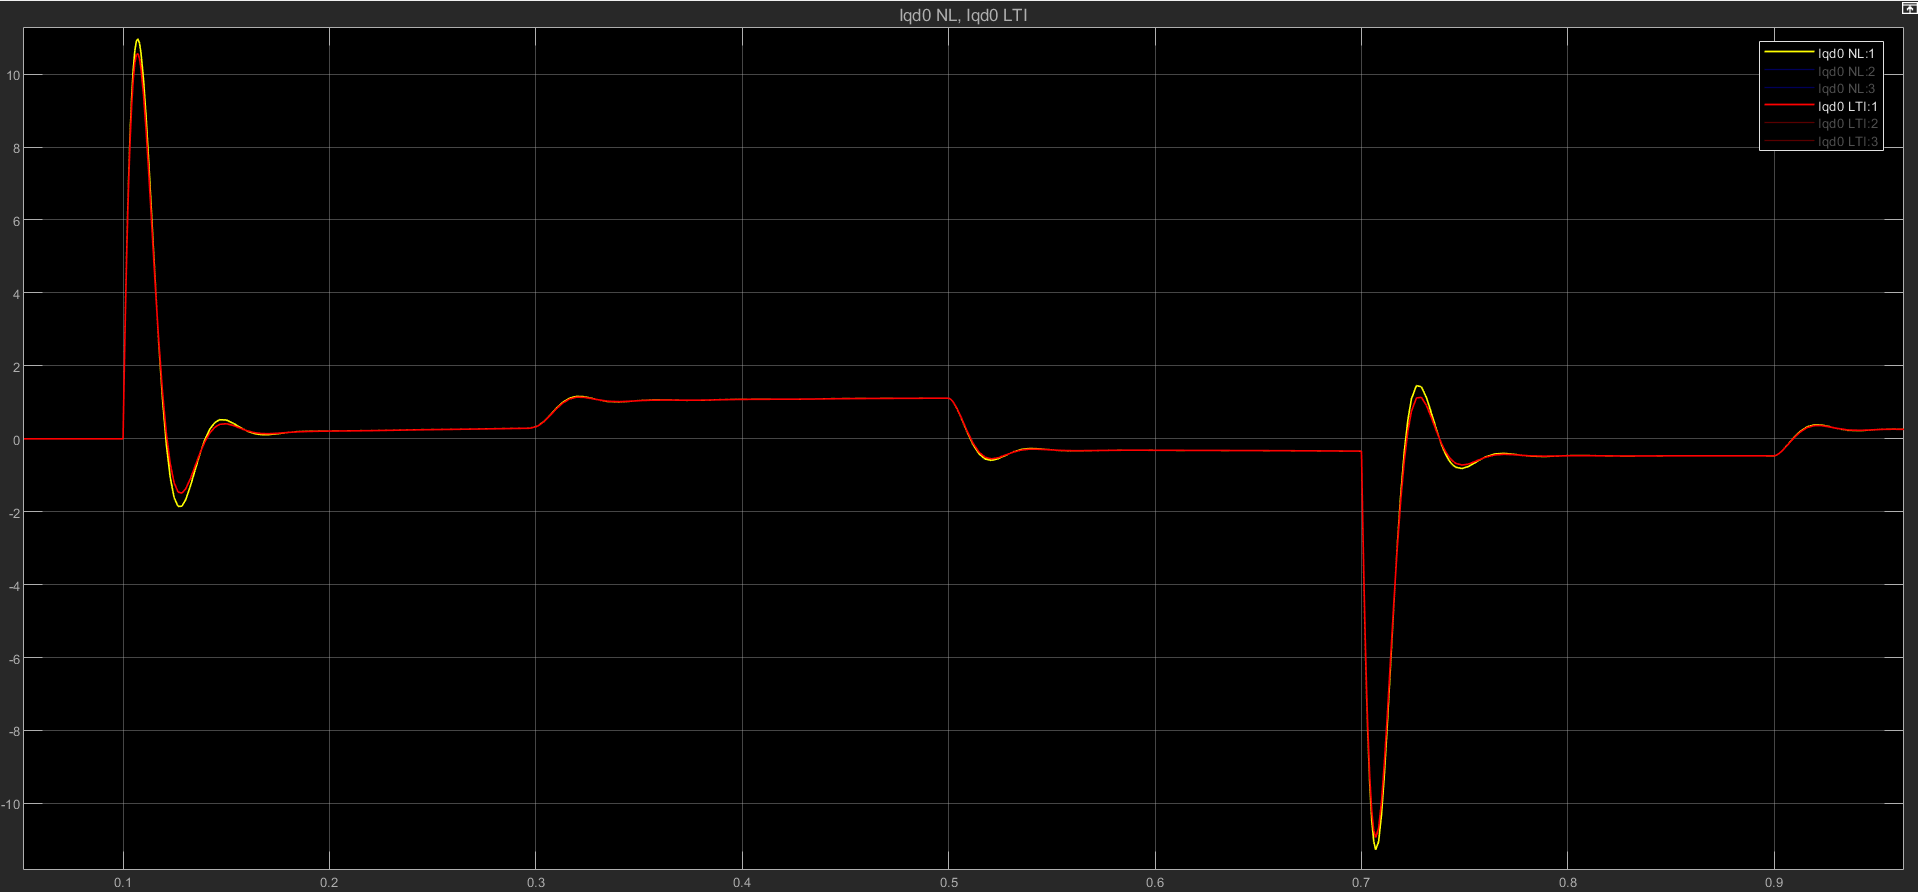
\includegraphics[width=1\textwidth]{Imagenes/ComparativaCorrientesVirtuales.png}
    \caption{Comparación de las corrientes virtuales entre el sistema NL y el sistema LTI aumentado. Amarillo: sistema NL - Rojo: sistema LTI aumentado.}
    \label{fig:ComparativaCorrientesVirtuales}
\end{figure}
\end{frame}

%% Curva paramétrica wm - Tm con transitorios
\begin{frame}{Curva Paramétrica Torque vs Velocidad}\small
La curva paramétrica $\omega_m$-$T_m$ representa el comportamiento dinámico del sistema, construida a partir de los pares ordenados $(\omega_m(t),T_m(t))$ correspondientes a la velocidad angular del eje mecánico y el torque electromagnético, respectivamente, para cada instante $t$ de simulación. En esta representación se identifican 6 puntos agudos que corresponden a estados de equilibrio del sistema dinámico bajo las condiciones de entrada especificadas. La curva se puede dividir en 5 segmentos, cada uno representado con un color diferente, que conectan pares sucesivos de puntos de equilibrio. Estos segmentos constituyen las trayectorias de transición del sistema, es decir, los conjuntos de puntos que describen la evolución temporal del sistema cuando se desplaza de un estado de equilibrio a otro. Esta visualización permite apreciar tanto los estados estacionarios como la dinámica transitoria del sistema en el espacio de estados $\omega_m$-$T_m$.    
\end{frame}

\begin{frame}{Curva Paramétrica Torque vs Velocidad}
    \begin{figure}[H]
    \centering
    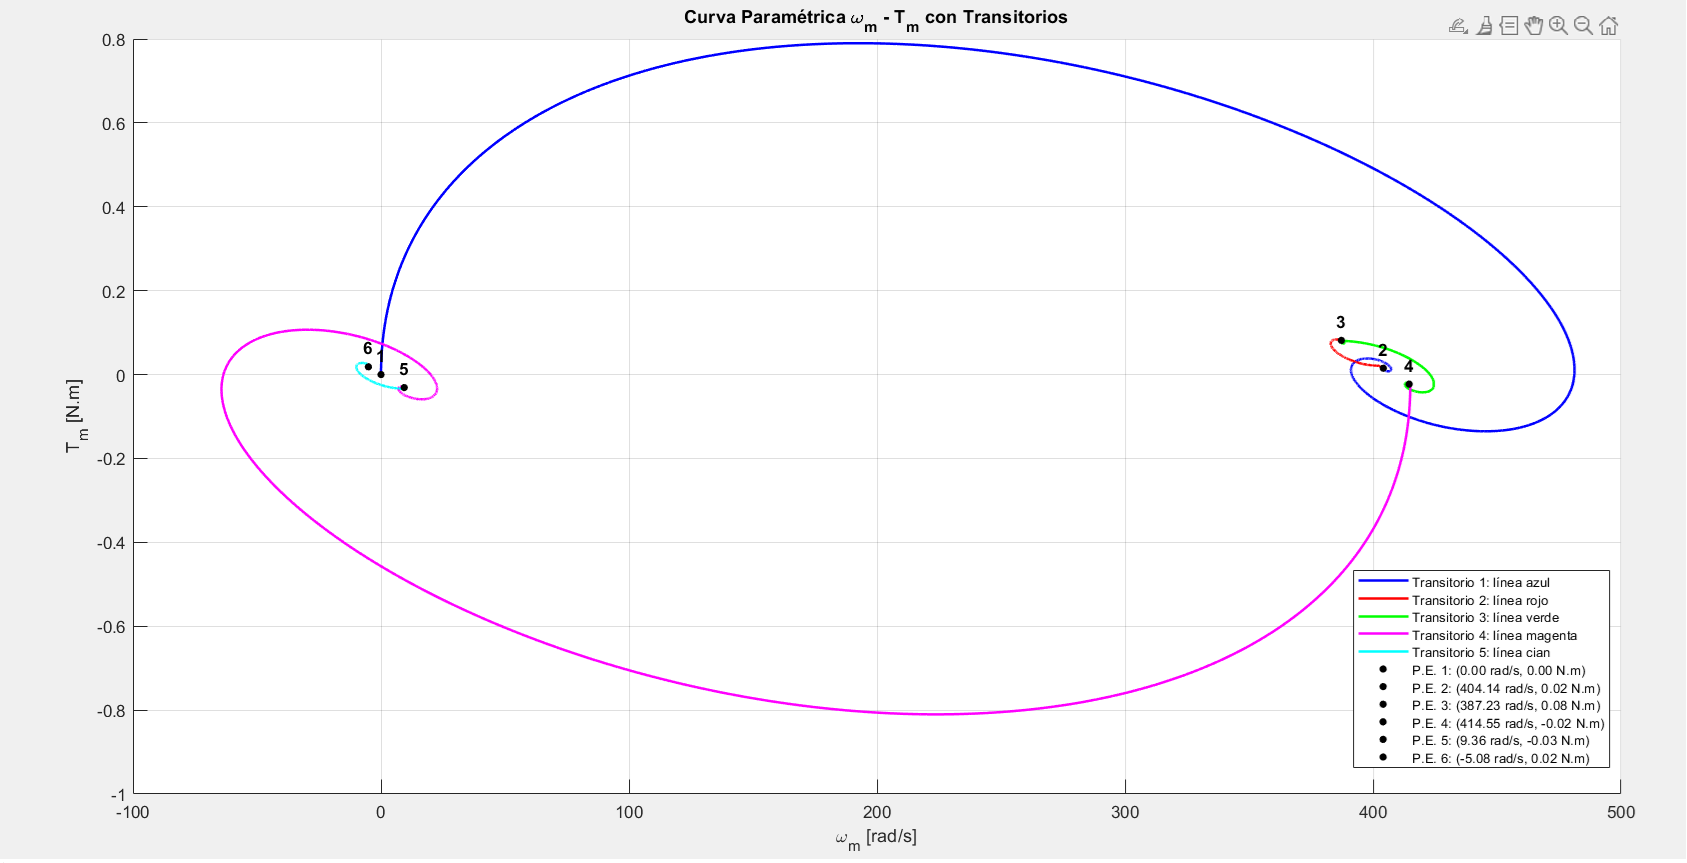
\includegraphics[width=1\textwidth]{Imagenes/CurvaParametricaWm-Tm.png}
    \caption{Curvas paramétricas de Torque vs Velocidad.}
    \label{fig:CurvaParametricaTorquevsVelocidad}
\end{figure}
\end{frame}

%% Determinación de velocidad y corriente final de establecimiento
\begin{frame}{\small Determinación de velocidad y corriente final de establecimiento} 
    \begin{table}[htbp]
    \tiny
   \centering
   \begin{tabular}{|c|c|c|c|c|c|}
       \hline
       \multicolumn{6}{|c|}{Parámetros del sistema} \\
       \hline
       & $V_q = 19.596V$ & $T_{ld} = 6.28\text{N.m}$ & $T_{ld} = -6.28\text{N.m}$ & $V_q = 0V$ & $T_{ld} = 0\text{N.m}$ \\
       & $t = 0.1\text{s}$ & $t = 0.3\text{s}$ & $t = 0.5\text{s}$ & $t = 0.7\text{s}$ & $t = 0.9\text{s}$ \\
       \hline
       $\omega_m$ Final [rad/s] & 403.90 & 387.1 & 414.50 & 9.50 & -5.35 \\
       \hline
       Tiempo de levantamiento $t_r$ [s] & 0.013 & 0.007 & 0.006 & 0.014 & 0.0071 \\
       \hline
       Tiempo de asentamiento $t_s$ [s] & 0.083 & 0.014 & 0.022 & 0.076 & 0.049 \\
       \hline
       Sobrepico [rad/s] & 77.27 & -7.161 & 4.046 & -55.442 & -2.5673 \\
       \hline
       \hline
       $i_q$ Final [A] & 0.2094 & 1.063 & -0.3155 & -0.468 & 0.2522 \\
       \hline
       Tiempo de levantamiento $t_r$ [s] & 0.000623 & 0.0145 & 0.0134 & 0.00039 & 0.004200 \\
       \hline
       Tiempo de asentamiento $t_s$ [s] & 0.094 & 0.055 & 0.0052 & 0.083828 & 0.0052 \\
       \hline
       Sobrepico [A] & 10.76 & 0.100 & -0.22 & -10.782 & 0.1314 \\
       \hline
   \end{tabular}
   \caption{Parámetros característicos de la respuesta dinámica del sistema ante variaciones de tensión y torque de carga}
   \label{table:parametros_sistema}
\end{table}
\end{frame}

% ----------------------------------------------------------------------------------

\title[Proyecto Global Integrador]{
Diseño, Análisis y Simulación con Controlador de Movimiento}

\frame{\titlepage}

% Slide: Desacoplamiento Completo
\begin{frame}{Modulador de Torque Equivalente} \footnotesize
\textbf{Objetivo:} Desacoplar las corrientes \( i_{qs}^r \), \( i_{ds}^r \) y \( i_{0s} \) mediante:
\begin{itemize}
    \item Compensación de retroalimentaciones físicas.
    \item Linealización para dinámicas rápidas y desacopladas.
\end{itemize}

\textbf{Ecuaciones Desacopladas:} 

Partimos del subsistema electromagnético en qd0:
\begin{equation}
\begin{aligned}
    v_{qs}^r(t) &= R_s(T_s^\circ(t))\,i_{qs}^r(t) \;+\; L_q \frac{d i_{qs}^r(t)}{dt} \;+\; [\lambda_m' + L_d i_{ds}^r(t)] P_p \omega_m(t),\\[6pt]
    v_{ds}^r(t) &= R_s(T_s^\circ(t))\,i_{ds}^r(t) \;+\; L_d \frac{d i_{ds}^r(t)}{dt} \;-\; L_q i_{qs}^r(t) P_p \omega_m(t),\\[6pt]
    v_{0s}(t) &= R_s(T_s^\circ(t))\,i_{0s}(t) \;+\; L_{ls} \frac{d i_{0s}(t)}{dt}.
\end{aligned}
\end{equation}

Estos lazos contienen las retroalimentaciones físicas naturales: 
términos que dependen de \(\omega_m(t)\), la resistencia variable con la temperatura \(R_s(T_s^\circ(t))\), y acoplamientos entre las corrientes \(i_{qs}^r(t)\) e \(i_{ds}^r(t)\).

\end{frame}

\begin{frame}{Modulador de Torque Equivalente} \small

\textbf{Objetivo} $\rightarrow$ desacoplar términos naturales realimentando tensiones $\rightarrow$ lograr relación directa entre entradas de referencia y derivadas de las corrientes.

Desarrollando llegamos a:

\[
L_q \frac{d i_{qs}^r(t)}{dt} = v_{qs}^{r*}(t), \quad
L_d \frac{d i_{ds}^r(t)}{dt} = v_{ds}^{r*}(t).
\]

\textbf{\footnotesize \underline{Comparación con la Linealización por Retroalimentación NL Completa:}} \
La estrategia previa imponía $\rightarrow$ \( i_{ds}^r(t)=0 \) para desacoplar el canal de flujo magnético. (Caso particular)\

\textbf{Ahora} el desacoplamiento es \textbf{más general} $\rightarrow$ compensamos términos no lineales y acoplamientos $\rightarrow$ modelo interno: corrientes responden casi independiente a las entradas \( v_{qs}^{r*}(t) \) y \( v_{ds}^{r*}(t) \).
Logramos alcanzar una dinámica $\uparrow$ rápida y robusta, permitiendo variar incluso \( i_{ds}^r(t) \) si se desea realizar $\rightarrow$ debilitamiento o reforzamiento de campo.
\end{frame}


% Slide: Efecto de Rs Variable
\begin{frame}{Efecto de \(R_s(T_s^\circ)\) en el Desempeño} 
\textbf{Comparativa:}
\begin{itemize}
    \item \(R_s\) Constante: Error estacionario por desacople incompleto.
    \item \(R_s\) Variable: Mejor respuesta a temperatura variable.
\end{itemize}

\begin{figure}[h]
    \centering
    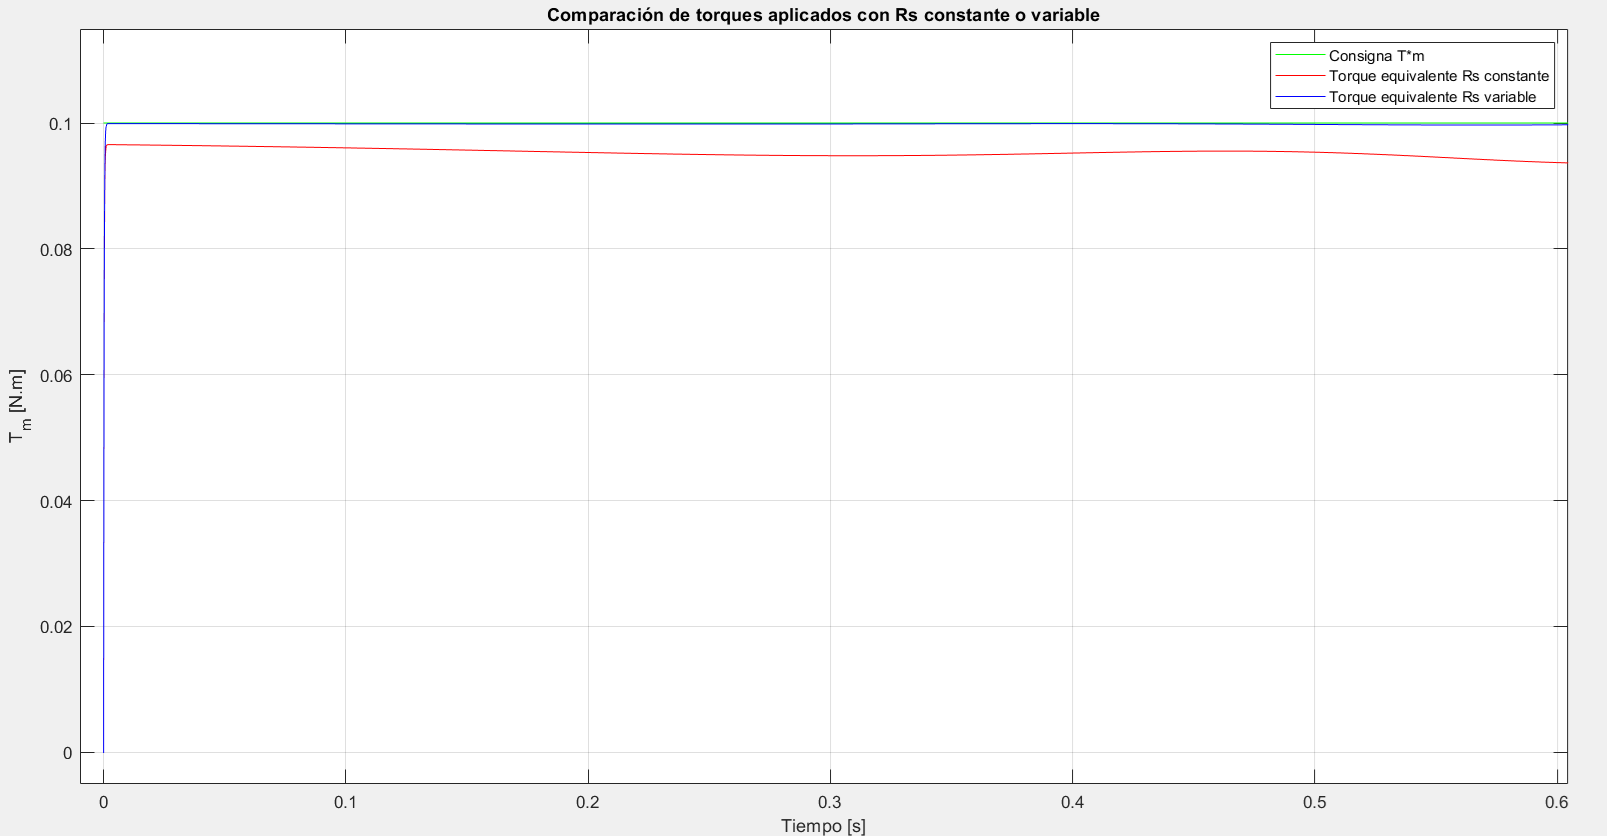
\includegraphics[width=0.65\textwidth]{Imagenes/ComparacionModuladorTorqueRs.png}
    \caption{Comparación del torque resultante sobre eje mecánico considerando \(R_s\) constante (rojo) y variable (azul).}
\end{figure}
Error estado estacionario: controlador no compensa variación. 
\end{frame}


\begin{frame}{Efecto de \(R_s(T_s^\circ)\) en el Desempeño}

Error que se refleja en la respuesta de velocidad:
\begin{figure}[h]
    \centering
    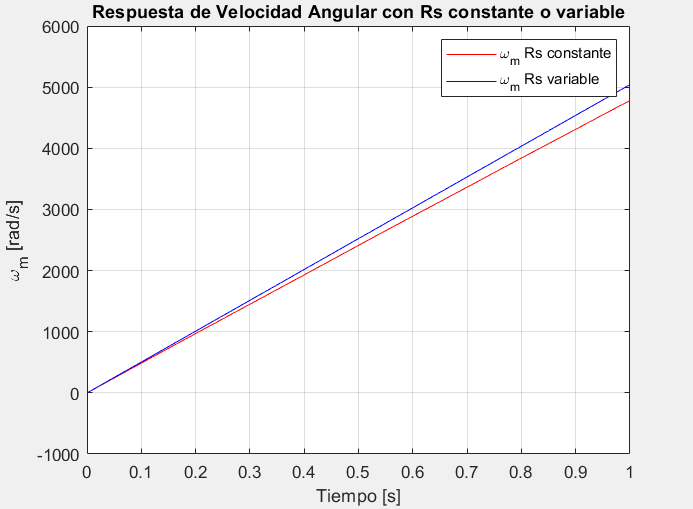
\includegraphics[width=0.65\textwidth]{Imagenes/ComparacionVelocidadModuladorRs.png}
    \caption{Comparación del torque resultante sobre el eje mecánico considerando \(R_s\) constante (rojo) y variable (azul).}
\end{figure}

Desvío progresivo entre curvas de velocidad angular \(\omega_m\):
\begin{itemize}
    \item Trayectoria con \(R_s\) constante (modelo simplificado).
    \item Trayectoria con \(R_s\) variable (incluye modelado térmico).
\end{itemize}

\medskip
Evidenciando el impacto del modelado térmico en el desempeño del sistema.
    
\end{frame}

\begin{frame}{Modulador de Torque Equivalente} \small

\textbf{Resultados:}
\begin{itemize} \footnotesize
    \item Dinámica interna linealizada. Relación: \textbf{tensiones virtuales} \((v_{qs}^{r*}(t), v_{ds}^{r*}(t), v_{0s}^{r*}(t))\) $\rightarrow$ \textbf{derivadas de las corrientes} \((i_{qs}^r(t), i_{ds}^r(t), i_{0s}(t))\)
    \item Corrientes responden directamente a las entradas de referencia.
\end{itemize}

\begin{figure}[h]
    \centering
    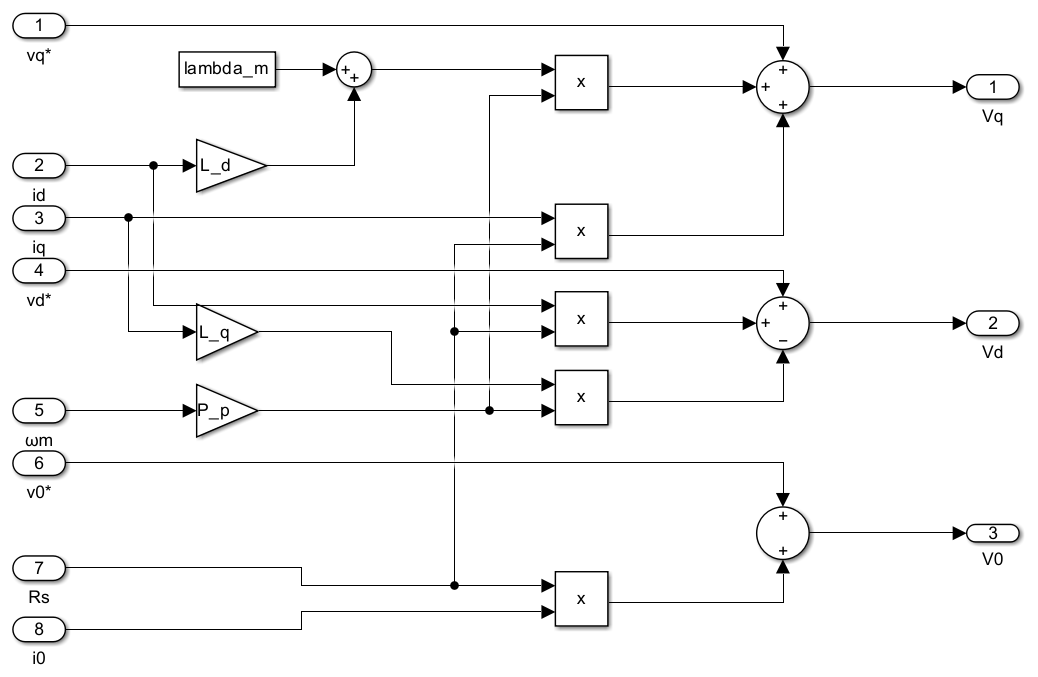
\includegraphics[width=0.55\textwidth]{Imagenes/modulador_torque_desacople_realimentaciones.png}
    \caption{Diagrama de bloques del modulador de torque.}
\end{figure}
\end{frame}


% Slide: Lazos de Corriente
\begin{frame}{\small Lazos de Control de Corrientes \(\boldsymbol{i^r_{q d 0 s}(t)}\) con Control Proporcional} \small
Para que el \textbf{modulador de torque equivalente} pueda \textbf{ejecutar correctamente} las \textbf{consignas de torque} $\rightarrow$ \textbf{necesario} asegurar \textbf{control directo y preciso} sobre las \textbf{corrientes} del estator \( qd0 \).

\vspace{0.5cm} % Espacio vertical

Por ello, implementamos lazos de control proporcionales de corriente. \
Objetivo: obtener \textbf{tensiones de referencia} \((v_{qs}^{r*}(t), v_{ds}^{r*}(t), v_{0s}^{r*}(t))\) a partir del \textbf{error} entre las \textbf{corrientes deseadas} \((i_{qs}^{r*}(t), i_{ds}^{r*}(t), i_{0s}^{r*}(t))\) y las \textbf{corrientes medidas} \((i_{qs}^r(t), i_{ds}^r(t), i_{0s}(t))\), \textbf{multiplicando} por una \textbf{ganancia proporcional} adecuada.

\end{frame}
\begin{frame}{Lazos de Control de Corrientes} \footnotesize

Partimos de:

\[
L_q \frac{d i_{qs}^r(t)}{dt} \approx v_{qs}^{r*}(t) = (i_{qs}^{r*}(t) - i_{qs}^r(t)) R'_q,
\]
\[
L_d \frac{d i_{ds}^r(t)}{dt} \approx v_{ds}^{r*}(t) = (i_{ds}^{r*}(t) - i_{ds}^r(t)) R'_d,
\]
\[
L_{ls} \frac{d i_{0s}(t)}{dt} \approx v_{0s}^{r*}(t) = (i_{0s}^{r*}(t) - i_{0s}(t)) R'_0.
\]

\(R'_q, R'_d, R'_0\) son \textbf{constantes de proporcionalidad} que, físicamente, pueden interpretarse como \textbf{resistencias virtuales}. \ 
Su elección determinará la \textbf{ubicación} de los \textbf{polos} del \textbf{lazo de corriente}.

\vspace{0.1cm} % Espacio vertical

Aplicando transformada de Laplace y funciones de transferencia, llegamos a:

\textbf{\underline{Lazos Proporcionales:}}
\[
G_{iqs}(s) = \frac{1}{\frac{L_q}{R'_q}s + 1}, \quad
G_{ids}(s) = \frac{1}{\frac{L_d}{R'_d}s + 1}, \quad
G_{i0s}(s) = \frac{1}{\frac{L_{ls}}{R'_0} s + 1}.
\]

Cada lazo de corriente $\rightarrow$ filtro pasa-bajos de primer orden.\
Polos determinado por las relaciones \(\frac{R'_q}{L_q}\), \(\frac{R'_d}{L_d}\), \(\frac{R'_0}{L_{ls}}\).

\end{frame}
\begin{frame}{\small Lazos de Control de Corrientes - Elección de Polos y Ganancias} \small

\textbf{Objetivo de diseño:}
\begin{itemize}
    \item Polos en \(p_i = -5000\,\text{rad/s}\).
    \item Respuesta rápida y robusta.
\end{itemize}

%Por lo tanto:\vspace{-0.3cm}
\begin{columns}
    % Columna de las ecuaciones
    \begin{column}{0.5\textwidth}
        Por lo tanto:
        \[
        \frac{R'_q}{L_q} = 5000 \implies R'_q = 5000 L_q = 29 \, \Omega,
        \]
        \[
        \frac{R'_d}{L_d} = 5000 \implies R'_d = 5000 L_d = 33 \, \Omega,
        \]
        \[
        \frac{R'_0}{L_{ls}} = 5000 \implies R'_0 = 5000 L_{ls} = 4 \, \Omega.
        \]
    \end{column}
    
    % Columna de la figura
    \begin{column}{0.5\textwidth}
        \centering
        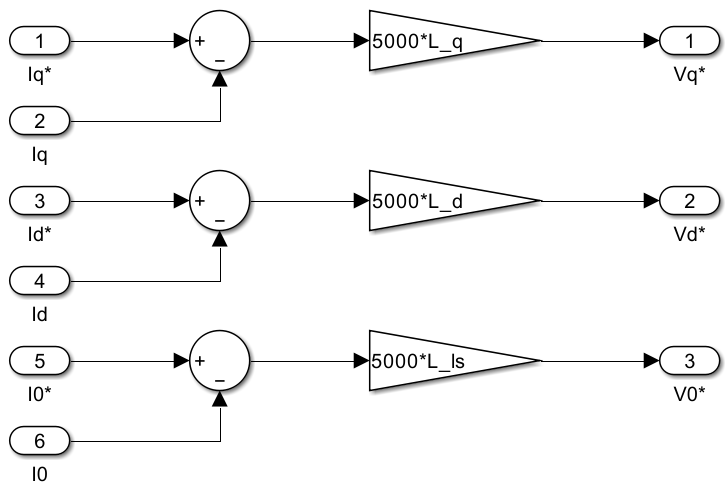
\includegraphics[width=0.9\textwidth]{Imagenes/modulador_corriente.png}
        \captionof{figure}{Diagrama de bloques del modulador de corriente.}
    \end{column}
\end{columns}

Extendiendo el ancho de banda hasta aproximadamente 796 Hz.
\end{frame}

\begin{frame}{Interpretación y Comparación}
A diferencia de la linealización mínima mediante retroalimentación no lineal, imponiendo \( i_{ds}^r(t)=0 \). Ahora nos \textbf{permite}:
\begin{itemize}
    \item Ajustar la velocidad de respuesta de las corrientes.
    \item Aumentar la robustez ante variaciones paramétricas (ejemplo \(R_s(T_s^\circ)\)).
    \item Permitir \( i_{ds}^{r*}(t) \neq 0 \), abriendo la posibilidad de realizar debilitamiento o reforzamiento de campo, algo que no era posible bajo la condición \(i_{ds}^r(t)=0\).
\end{itemize}
\end{frame}


% Diapositiva 1: Introducción
\begin{frame}{Incorporación de la Consigna de Torque y Compensación del Subsistema Mecánico}
    \begin{itemize}
        \item Incorporación de la consigna de torque mecánico como nueva variable manipulada.
        \item Compensación de perturbaciones mecánicas internas:
        \begin{itemize}
            \item Fricción viscosa equivalente.
            \item Torque gravitacional sobre la carga.
        \end{itemize}
        \item Garantía de que el torque electromagnético del lazo externo de control de movimiento no se vea afectado.
    \end{itemize}
\end{frame}

% Diapositiva 2: Consigna de Torque con Compensación
\begin{frame}{Consigna de Torque con Compensación de Fricción Viscosa y Gravedad}
    \textbf{Precomputed Torque:}
    \begin{itemize}
        \item Se parte de una consigna de torque pura: $T_m^{*'}(t)$.
        \item Se incluyen compensaciones mecánicas para fricción y gravedad:
    \end{itemize}
    \begin{equation}
        T_m^{*}(t) = T_m^{*'}(t) + b_{eq}\,\omega_m(t) + \frac{k_t}{r}\sin\left(\frac{\theta_m(t)}{r}\right).
    \end{equation}
    \begin{itemize}
        \item Facilita el diseño del controlador de movimiento.
        \item Reduce la carga computacional del control externo.
    \end{itemize}
\end{frame}

% Diapositiva 3: Relación entre Torque y Corrientes
\begin{frame}{Relación entre el Torque y las Corrientes}
    \textbf{Expresión del torque electromagnético en coord. qd:}
    \begin{equation}
        T_m(t) = \frac{3}{2} P_p [ \lambda_m' + (L_d - L_q)i_{ds}^r(t) ]\, i_{qs}^r(t).
    \end{equation}
    Conocido \(T_m^{*}(t)\), despejamos la referencia de corriente en el eje q: \
    \begin{equation}
        i_{qs}^{r*}(t) = \frac{T_m^{*'}(t) + b_{eq}\,\omega_m(t) + \frac{k_l \cdot g}{r}\sin\left(\frac{\theta_m(t)}{r}\right)}{\frac{3}{2}P_p[\lambda_m' + (L_d - L_q)i_{ds}^r(t)]}.
    \end{equation}
\end{frame}

% Diapositiva 4: Casos Especiales y Flexibilidad
\begin{frame}{Casos Especiales y Flexibilidad}
    \begin{itemize}
        \item Si $i_{ds}^r(t)=0$, el torque depende solo del flujo del imán permanente y la corriente q.
        \begin{itemize}
            \item Configuración simple y eficiente.
        \end{itemize}
        \item Si $i_{ds}^r(t)\neq 0$, permite modificar el campo magnético interno.
        \begin{itemize}
            \item Expande el rango de operación en torque y velocidad.
            \item Implica mayor complejidad en control.
        \end{itemize}
    \end{itemize}
\end{frame}

% Diapositiva 5: Diagrama del Modulador de Torque
\begin{frame}{Diagrama del Modulador de Torque}
    \begin{figure}[H]
        \centering
        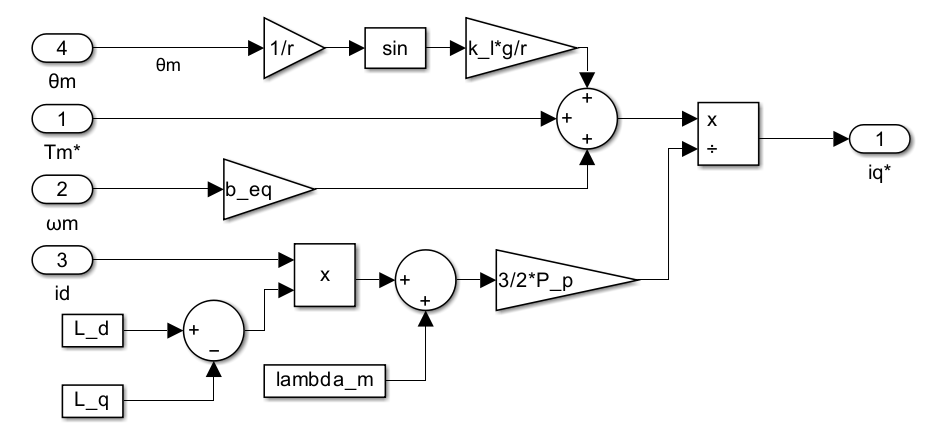
\includegraphics[width=0.7\textwidth]{Imagenes/modulador_torque.png}
        \caption{Diagrama de bloques del modulador de torque con compensaciones internas.}
        \label{fig:modulador_torque_1}
    \end{figure}
\end{frame}

% Diapositiva 8: Simulación con Modulador de Torque
\begin{frame}{Simulación con Modulador de Torque}
    \begin{itemize}
        \item Evaluación en el dominio del tiempo del sistema global con el modulador de torque diseñado.
        \item Se comparan las señales de torque electromagnético, torque aplicado, perturbaciones y fricción viscosa.
    \end{itemize}
    \begin{figure}[H]
        \centering
        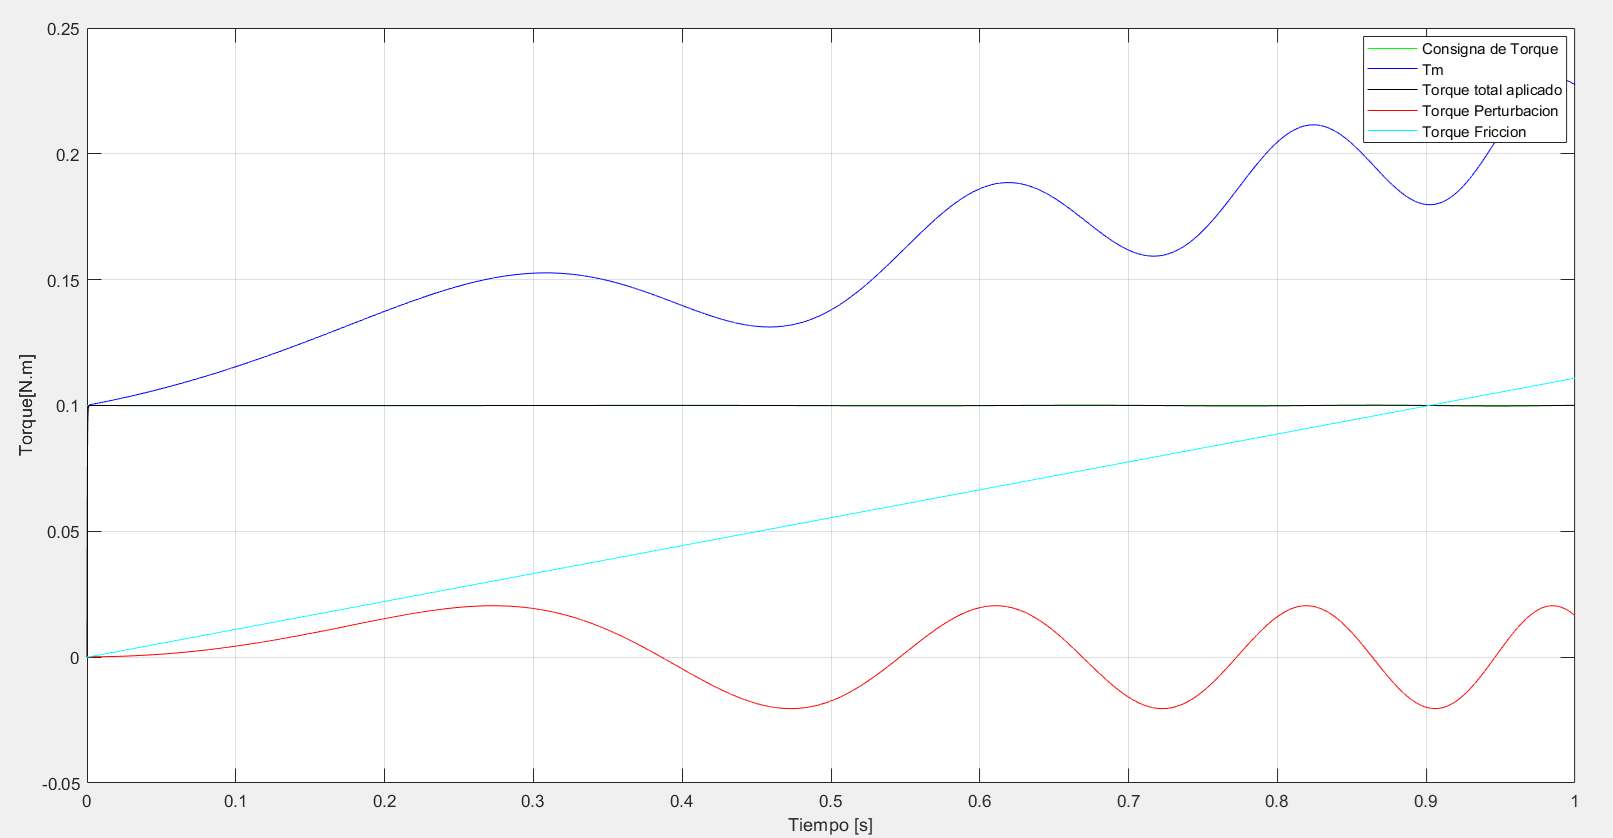
\includegraphics[width=0.7\textwidth]{Imagenes/Torques_simulacion_modulador_torque.png}
        \caption{Comparación de torques en la simulación con modulador de torque.}
        \label{fig:curvas_torques_modulador}
    \end{figure}
\end{frame}

% Diapositiva 9: Seguimiento de Consigna de Torque
\begin{frame}{Seguimiento de Consigna de Torque}
    \begin{itemize}
        \item El torque total aplicado sigue el escalón de la consigna de torque.
        \item Se requiere compensación del torque de perturbación y fricción viscosa.
    \end{itemize}
    \begin{figure}[H]
        \centering
        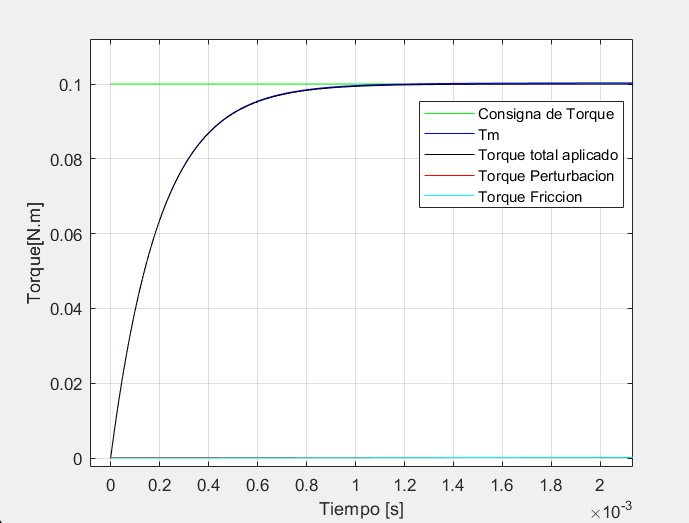
\includegraphics[width=0.55\textwidth]{Imagenes/Acercamiento_torques_modulador.png}
        \caption{Acercamiento en el instante inicial mostrando respuesta del torque total aplicado.}
        \label{fig:acercamiento_torques_modulador}
    \end{figure}
\end{frame}

% Diapositiva 10: Respuesta en Posición y Velocidad
\begin{frame}{Respuesta en Posición y Velocidad}
    \begin{itemize}
        \item Un torque constante genera una aceleración angular constante.
        \item La velocidad angular sigue una trayectoria lineal, mientras que la posición tiene una curva parabólica.
    \end{itemize}
    \begin{figure}[H]
        \centering
        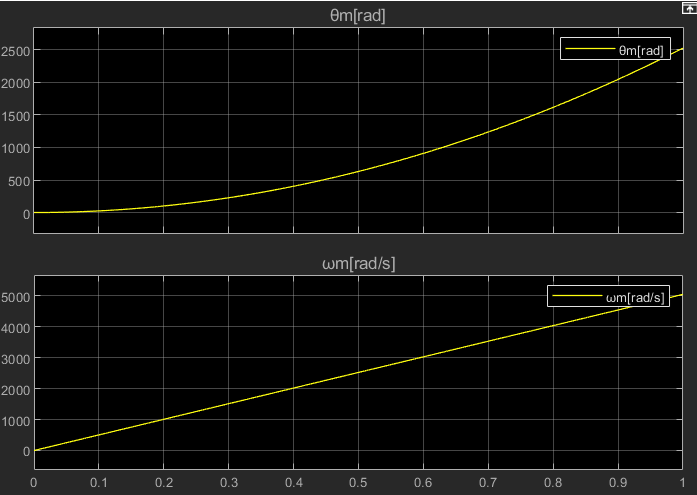
\includegraphics[width=0.6\textwidth]{Imagenes/Curvas_posicion_velocidad_modular_torque.png}
        \caption{Curvas de posición y velocidad angular del eje mecánico.}
        \label{fig:curvas_posicion_velocidad_modulador_torque}
    \end{figure}
\end{frame}

% Diapositiva 11: Respuesta de Corrientes
\begin{frame}{Respuesta de Corrientes en Coordenadas abc}
    \begin{itemize}
        \item El torque electromagnético representa la envolvente de las corrientes reales.
        \item Crecimiento de corriente debido a la compensación de fricción viscosa.
    \end{itemize}
    \begin{figure}[H]
        \centering
        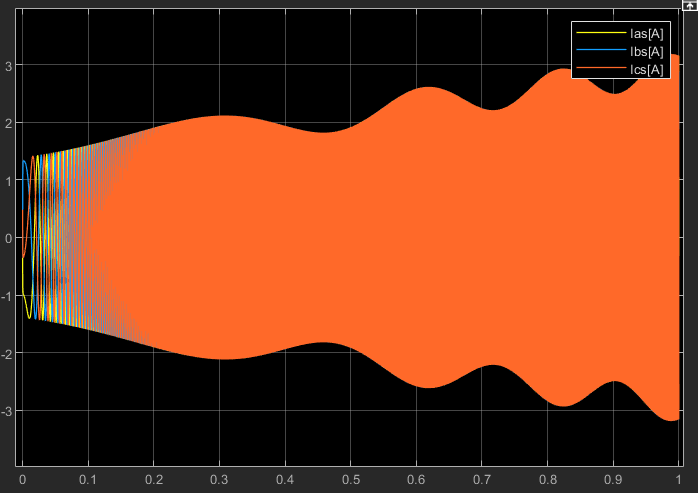
\includegraphics[width=0.48\textwidth]{Imagenes/Curvas_corrientes_modulador_torque.png}
        \caption{Corrientes en coordenadas $abc$ con modulador de torque.}
        \label{fig:curvas_corrientesABC_modulador_torque}
    \end{figure}
\end{frame}

% Diapositiva 12: Efectos de i_{ds} en el Torque
\begin{frame}{Efectos de $i_{ds}^*(t)$ en el Torque}
De la ecuación \textbf{$i_{qs}^{r*}(t)$} concluimos que:
    \begin{itemize}
        \item $i_{ds}^*(t) = 0$: Torque solo depende del flujo de imanes permanentes.
        \item $i_{ds}^*(t) \neq 0$:
        \begin{itemize}
            \item $i_{ds}^*(t) > 0$ refuerza el campo y aumenta el torque.
            \item $i_{ds}^*(t) < 0$ debilita el campo y reduce el torque.
        \end{itemize}
    \end{itemize}
\end{frame}


% Diapositiva 13: Controlador Externo de Movimientos
\begin{frame}{Controlador Externo de Movimientos: Posición/Velocidad}
    \begin{itemize}
        \item Para \textbf{mejorar dinámica} del sistema y \textbf{corregir errores de estado estacionario} por cargas perturbadoras \textbf{$\rightarrow$} se \textbf{implementa controlador} que recibe \textbf{consignas} de \textbf{velocidad y posición}.
        \item Define el torque necesario para la acción requerida.
        \item Método de sintonía serie con acción integral para el PID.
        \item Parámetros: $\xi = 0.75$, $\omega_n = 800\, {rad/s}$. Valores nominales de $J_l$ y $b_l$.
    \end{itemize}
\end{frame}

% Diapositiva 14: Diseño del Controlador
\begin{frame}{Diseño del Controlador PID}
    \begin{itemize}
        \item Se elige como variable de entrada la velocidad angular del motor.
        \item Evita acciones derivativas para reducir errores numéricos.
        \item Dos bloques integrales actúan como filtros pasa bajos para eliminar ruido.
    \end{itemize}
    \begin{figure}[H]
        \centering
        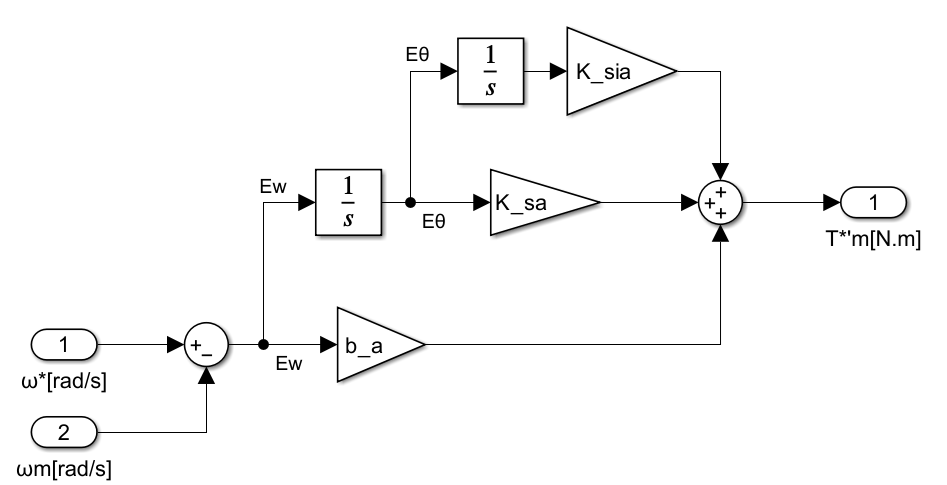
\includegraphics[width=0.5\textwidth]{Imagenes/DiagramaBloquesPIDdesagregado.png}
        \caption{Diagrama de bloques del controlador PID}
\label{fig:DiagramaBloquesPIDdesagregado}
    \end{figure}

Salida:\
    \begin{equation}
T_m^{*'}(s) = e_\omega(s).b_a + e_\theta(s).K_{sa} + K_{sia}\frac{e_\theta(s)}{s}
\label{eq:torque_controlador}
\end{equation}
\end{frame}

% Diapositiva 15: Relación entre Torque y Velocidad
\begin{frame}{Relación entre Torque y Variación de Velocidad}
    \textbf{Ecuación dinámica del subsistema mecánico:}
    \begin{equation}
        J_{eq}\dot{\omega}_m(t) = T_m^*(t) - \frac{T_l(t)}{r}
    \end{equation}
    \begin{itemize}
        \item Se considera el desacople de $-b_{eq}\omega_m(t)$.
        \item Modelado en el dominio de Laplace:
        \begin{equation}
            J_{eq} \cdot s^2 \cdot \theta_m(s) = T_m^*(s) - \frac{T_l(s)}{r}
        \end{equation}
    \end{itemize}
\end{frame}

% Diapositiva 16: Expresión del Torque del Controlador
\begin{frame}{Expresión del Torque del Controlador}
    \begin{itemize}
        \item Sustituyendo el torque del controlador:
        \begin{equation}
            J_{eq} \cdot s^2 \cdot \theta_m(s) = E_\theta(s) \cdot s \cdot b_a + E_\theta(s) \cdot K_{sa} + \frac{E_\theta(s)}{s} \cdot K_{sia} - \frac{T_l(s)}{r}
        \end{equation}
        \item Expandiendo el error de posición:
        \begin{equation}
            J_{eq} \cdot s^2 \cdot \theta_m(s) = \left[s \cdot b_a + K_{sa} + \frac{K_{sia}}{s}\right] \cdot [\theta_m^*(s) - \theta_m(s)] - \frac{T_l(s)}{r}
        \end{equation}
    \end{itemize}
    Agrupando términos y finalmente despejando $\theta_m(s)$, identificamos:
\end{frame}

% Diapositiva 17: Funciones de Transferencia del Controlador
\begin{frame}{Funciones de Transferencia del Controlador}
    \textbf{Para la entrada de consigna de posición:}
    \begin{equation}
        G_{\theta^*_m}(s) = \frac{s^2 b_a + s K_{sa} + K_{sia}}{J_{eq} s^3 + s^2 b_a + s K_{sa} + K_{sia}}
    \end{equation}
    \textbf{Para la perturbación de torque:}
    \begin{equation}
        G_{T_l}(s) = -\frac{s}{J_{eq} s^3 + s^2 b_a + s K_{sa} + K_{sia}}
    \end{equation}
    \begin{itemize}
        \item La ecuación $G_{\theta^*_m}(s)$ describe la respuesta a cambios en la consigna de posición.
        \item La ecuación $G_{T_l}(s)$ muestra la influencia de perturbaciones en el torque de carga.
    \end{itemize}
\end{frame}

% Diapositiva 18: Respuesta en Régimen Estacionario
\begin{frame}{Respuesta en Régimen Estacionario}
    \begin{itemize}
        \item Evaluando las funciones de transferencia en régimen estacionario para una entrada escalón unitario:
        \begin{itemize}
            \item Si $K_{sia} \neq 0 \Rightarrow G_{\theta^*}(s) = 1$ y $G_{T_l}(s) = 0$ (rechazo total a perturbaciones).
            \item Si $K_{sia} = 0 \Rightarrow G_{\theta^*}(s) = 1$ y $G_{T_l}(s) = -1/K_{sa}$ (sin rechazo a perturbaciones).
        \end{itemize}
        \item Concluimos: La acción integral es clave para la eliminación de errores en estado estacionario.
    \end{itemize}
\end{frame}

% Diapositiva 18: Sintonización del Controlador
\begin{frame}{Sintonización del Controlador}
Buscamos valores óptimos de las ganancias del controlador:
    \begin{itemize}
        \item Método de sintonía serie con $n = 2.5$.
        \item Cálculo de ganancias con $J_{eq}$ nominal.
        \item Definición de frecuencias características:
        \begin{equation}
            \omega_{vel} = \frac{b_a}{J_{eq}}, \quad \omega_{pos} = \frac{K_{sa}}{b_a}, \quad \omega_{int} = \frac{K_{sia}}{K_{sa}}
        \end{equation}
    \end{itemize}
    \textbf{Ganancias calculadas:}
    \begin{equation}
        b_a = 0.039 \frac{N \cdot m}{rad/s}, \quad K_{sa} = 31.656 \frac{N \cdot m}{rad}, \quad K_{sia} = 10129.78 \frac{N \cdot m}{rad \cdot s}
    \end{equation}
    Con ello, obtenemos el polinomio característico del controlador y comparamos con la forma normalizada $\rightarrow$ distintos polos
\end{frame}

% Diapositiva 19: Migración de Polos del Controlador
\begin{frame}{Migración de Polos del Controlador}
    \begin{itemize}
        \item Se analizan los polos del sistema para diferentes valores de $J_{eq}$ y $b_{eq}$.
        \item Comparación con los polos del lazo de corriente y de la planta original en lazo abierto.
    \end{itemize}
    \begin{figure}[H]
        \centering
        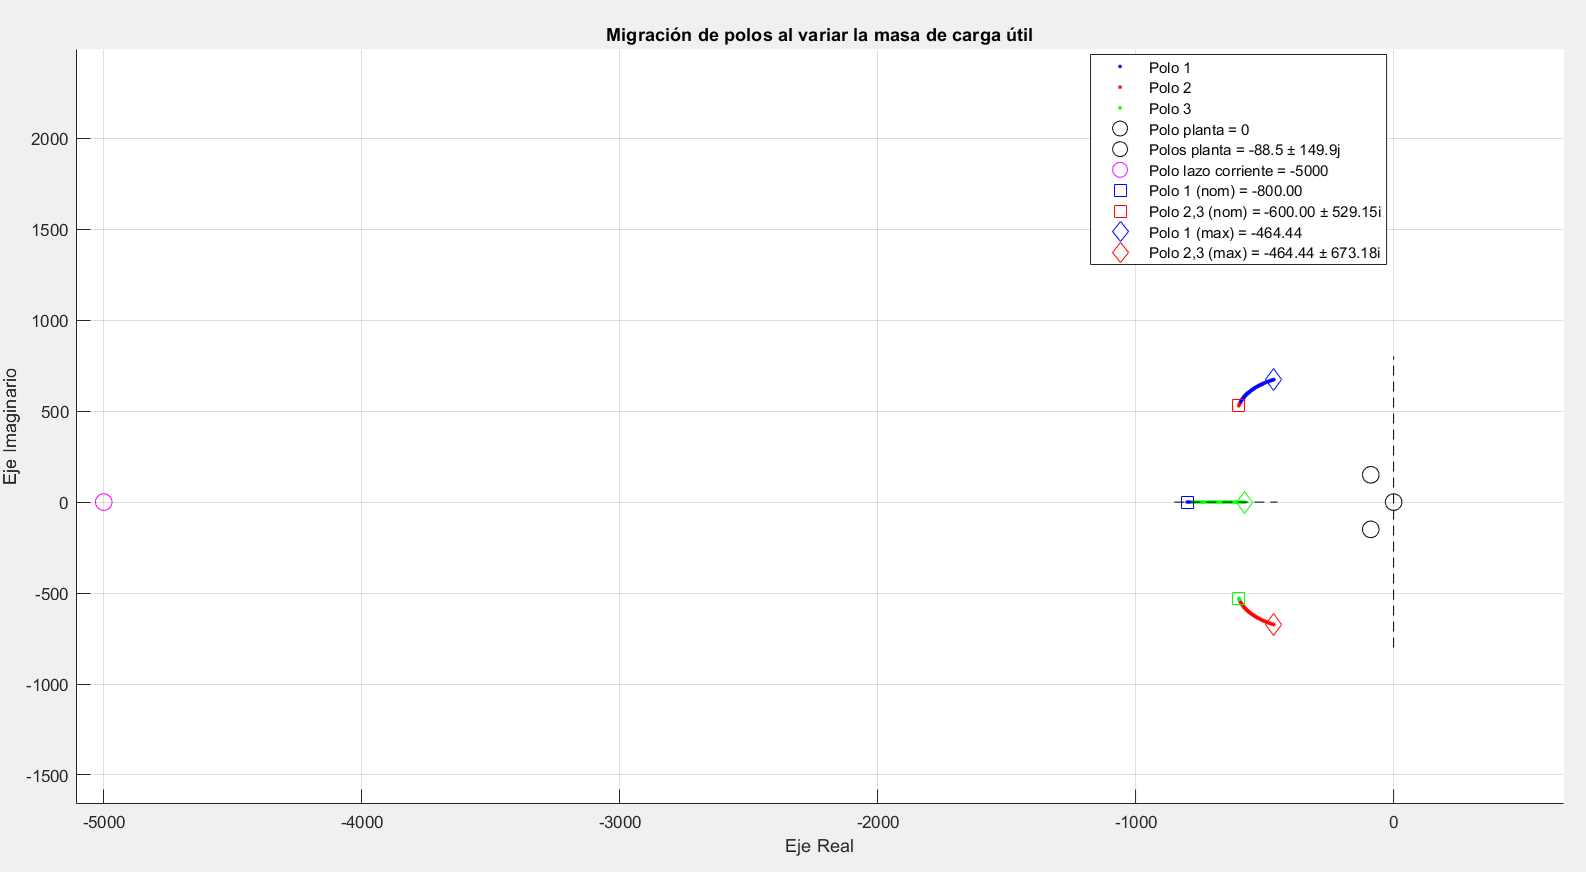
\includegraphics[width=0.9\textwidth]{Imagenes/MigracionPolosControlador.png}
        \caption{Polos del controlador variando $J_{eq}$ y $b_{eq}$.}
        \label{fig:migracion_polos_controlador}
    \end{figure}
\end{frame}

% Diapositiva 20: Setpoint de Posición
\begin{frame}{Setpoint de Posición}
    \begin{itemize}
        \item Implementación del control de posición mediante referencia de consigna.
        \item Generación de una consigna de velocidad a partir de la derivada de la posición de referencia.
        \item Evita amplificación de ruido debido a su origen en la consigna y no en mediciones.
    \end{itemize}
    \begin{figure}[H]
        \centering
        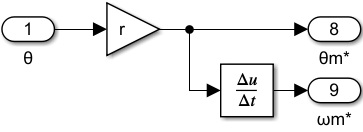
\includegraphics[width=0.5\textwidth]{Imagenes/setpoint.png}
        \caption{Diagrama de bloques del setpoint de posición $\theta_m^*$.}
        \label{fig:setpoint}
    \end{figure}
\end{frame}


% Slide: Introducción al Observador
\begin{frame}{Observador de Estado de Orden Reducido}
\textbf{Propósito:}
\begin{itemize}
    \item Estimar \(\omega_m(t)\) a partir de \(\theta_m(t)\).
    \item Evitar el uso de sensores de velocidad.
    \item Mejorar el control externo mediante estimaciones rápidas y precisas.
\end{itemize}

\textbf{Modelo del Subsistema Mecánico:}
\[
\dot{x}(t) = 
\begin{bmatrix}
0 & 1 \\ 
0 & 0
\end{bmatrix} 
x(t) + 
\begin{bmatrix}
0 \\ 
\frac{1}{J_{eq}}
\end{bmatrix} 
u(t), \quad
y(t) = 
\begin{bmatrix}
1 & 0
\end{bmatrix} 
x(t).
\]

\textbf{Estados Iniciales:}
\[
e(0) = x(0) - \tilde{x}(0), \quad \dot{e}(t) = (A - K_eC)e(t).
\]
\end{frame}


% Slide: Diseño del Observador
\begin{frame}{Diseño del Observador}
\textbf{Ecuación del Observador: (basado en la estructura de Luenberger)}
\[
\dot{\tilde{x}}(t) = A \tilde{x}(t) + Bu(t) + K_e\left[y(t) - C\tilde{x}(t)\right].
\]

\textbf{Cálculo de \( K_e \):}
\[
A - K_e C = \begin{bmatrix} 
-K_{e\theta} & 1 \\ 
-K_{e\omega} & 0 
\end{bmatrix}.
\]
\[
p(s) = \det\left(sI - (A - K_e C)\right) = s^2 + K_{e\theta}s + K_{e\omega}.
\]
Para \( p_{\text{obs}} = -3200 \, \text{rad/s} \), el polinomio característico deseado es:
\[
p_{\text{obs}}(s) = (s + 3200)^2 = s^2 + 6400s + 3200^7.
\]
Finalmente,
\[
K_{e\theta} = 6400 \, \text{rad/s}, \quad K_{e\omega} = 1.024 \times 10^7 \, \text{rad/s}^2.
\]
\end{frame}

\begin{frame}{Justificación de los Polos}\small
   \textbf{Justificación:}
\begin{itemize}
    \item Polos reales en \(-3200 \, \text{rad/s}\) para rápida convergencia.
    \item Ubicación separada de los polos del controlador externo.
\end{itemize}

\begin{figure}[h]
    \centering
    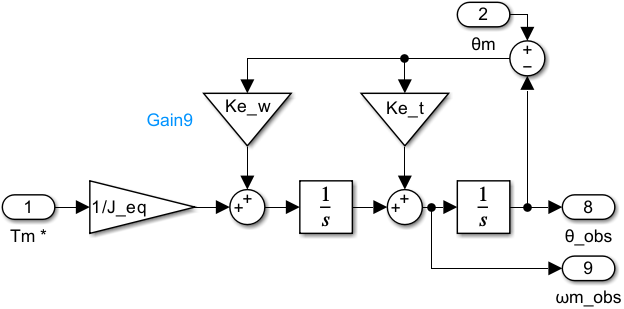
\includegraphics[width=0.5\textwidth]{Imagenes/observador.png}
\end{figure} 

\textbf{Análisis del Error:}
Gobernada por:
\[
\dot{e}(t) = (A - K_e C) e(t),
\]
donde \( A - K_e C \) es estable por construcción, con polos en \(-3200 \, \text{rad/s}\). Esto asegura que: \lim_{t \to \infty} e(t) = 0
\end{frame}

% Slide: Modelo Completo
\begin{frame}{Simulación - Modelo Completo NL}\small
\textbf{Componentes Principales:}
\begin{itemize}
    \item Planta: Subsistemas electromagnético, mecánico y térmico.
    \item Control: PID, modulador de torque, observador de estado.
\end{itemize}

\begin{figure}[h]
    \centering
    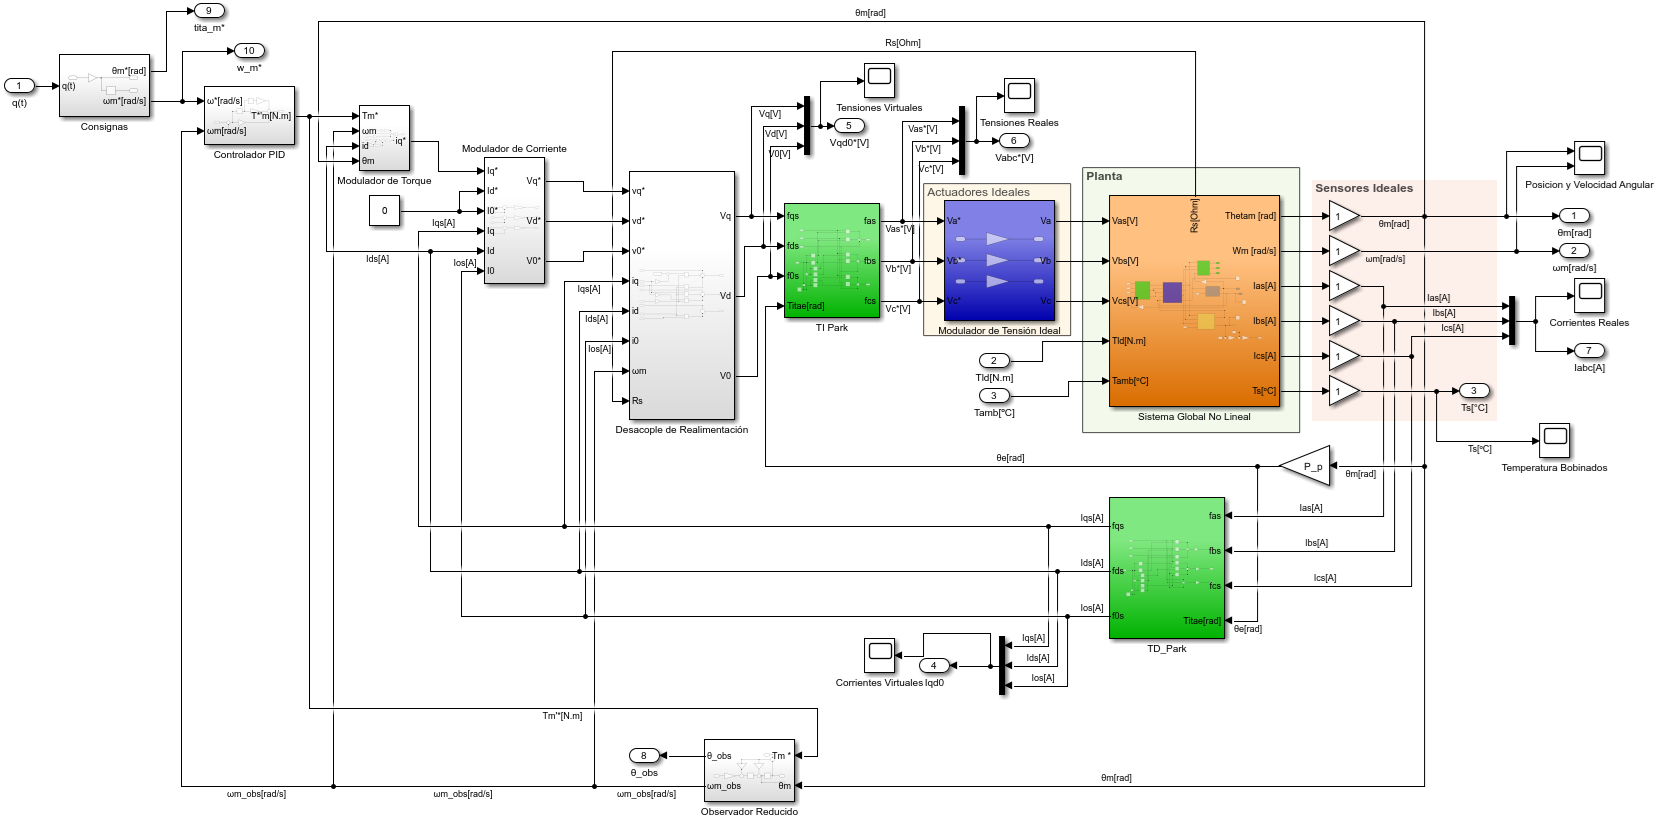
\includegraphics[width=1\textwidth]{Imagenes/Modelo_Completo_Simulacion.png}
\end{figure}
\end{frame}

% Diapositiva 24: Seguimiento de Consignas de Movimiento
\begin{frame}{Seguimiento de Consignas de Movimiento}
    \begin{itemize}
        \item Perfil trapezoidal de posición con $\Delta t_{ramp} = 5s$, $q^*(\Delta t_{ramp}) = 2\pi$rad.
        \item Movimientos de ida y vuelta de una vuelta completa.
    \end{itemize}
    \begin{figure}[H]
        \centering
        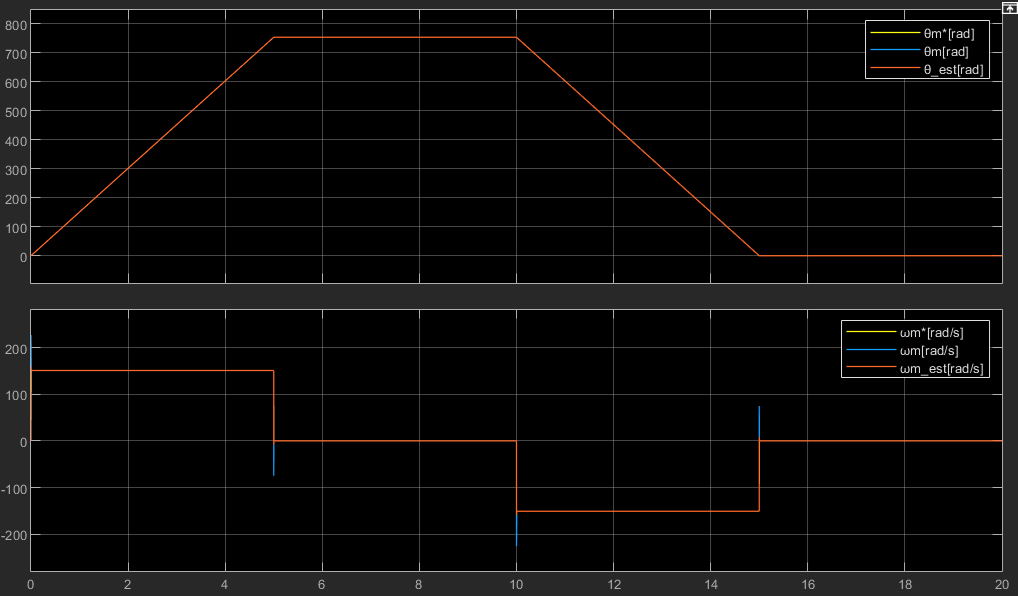
\includegraphics[width=0.8\textwidth]{Imagenes/PosicionVelocidadSimulacionModeloCompleto.png}
    \end{figure}
\end{frame}

% Slide: Seguimiento de Consignas
\begin{frame}{Seguimiento de Consignas de Movimiento}
\textbf{Consigna:}
  Movimiento trapezoidal en \(q^*(t)\) con \(\Delta t_{ramp} = 5\,s\), posición final \(2\pi \, \text{rad}\).


\begin{figure}[h]
    \centering
    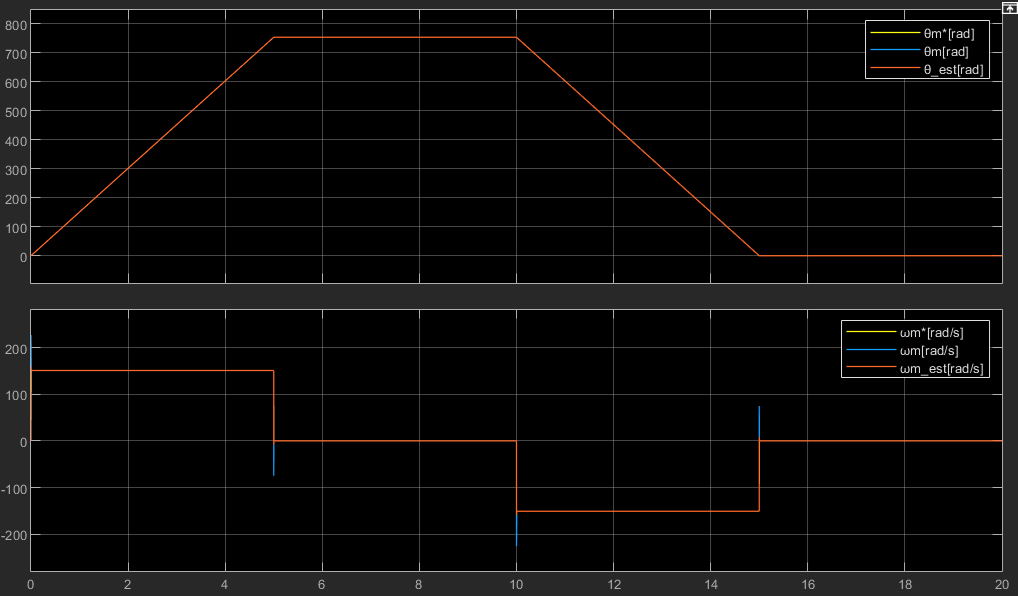
\includegraphics[width=0.7\textwidth]{Imagenes/PosicionVelocidadSimulacionModeloCompleto.png}
\end{figure}
\begin{itemize}\small
    \item Seguimiento exitoso, aunque con errores en transitorios.
    \item Perfiles trapezoidales presentan problemas prácticos: altas aceleraciones y picos de torque.
\end{itemize}
\end{frame}

\begin{frame}{Seguimiento de Consignas de Movimiento}
    \begin{figure}[h]
    \centering
    \includegraphics[width=0.95\textwidth]{Imagenes/AcercamientoRespuestaSimulacionCompleta.png}
    \caption{Acercamiento en el instante \(t = 5\,s\) para observar los transitorios de posición y velocidad.}
\end{figure}
\end{frame}

\begin{frame}{Seguimiento de Consignas de Movimiento}
    \begin{figure}[h]
    \centering
    \includegraphics[width=0.8\textwidth]{Imagenes/ErroresObservadorSimulacionCompleta.png}
    \caption{Error de posición y velocidad por estimación de Observador de Estado de Orden Reducido.}
\end{figure}
\end{frame}


% Diapositiva 27: Análisis de Tensiones en la Simulación
\begin{frame}{Análisis de Tensiones en la Simulación}
    \begin{itemize}
        \item En transitorios, se evidencian picos elevados que superan los límites de operación eléctrica.
        \item En la práctica, el modulador de tensión alcanzaría la saturación.
    \end{itemize}
    \begin{figure}[H]
        \centering
        \includegraphics[width=0.65\textwidth]{Imagenes/TensionesSimulacionCompleta.png}
        \caption{Curvas de tensiones en coordenadas virtuales y absolutas.}
    \end{figure}
\end{frame}

% Diapositiva 28: Acercamiento a Tensiones en Estado Estacionario y Transitorios
\begin{frame}{Análisis de Tensiones en la Simulación}
    \begin{itemize}
        \item En estado estacionario, las tensiones presentan un comportamiento senoidal.
        \item Se observan picos elevados en los transitorios, lo que genera sobrecargas.
    \end{itemize}
    \begin{figure}[H]
        \centering
        \includegraphics[width=0.6\textwidth]{Imagenes/AcercamientoTensionesEstacionariasSimulacion.png}
        \caption{Acercamiento: Tensiones en estados de eq.}
    \end{figure}
\end{frame}

\begin{frame}{Análisis de Tensiones en la Simulación}
    
    \begin{figure}[H]
        \centering
        \includegraphics[width=0.85\textwidth]{Imagenes/AcercamientoTensionesTransitoriosSimulacion.png}
        \caption{Acercamiento: Tensiones en transitorios.}
    \end{figure}
\end{frame}


% Diapositiva 29: Análisis de Corrientes en la Simulación
\begin{frame}{Análisis de Corrientes en la Simulación}
    \begin{itemize}
        \item En estado estacionario, las corrientes presentan comportamiento senoidal.
        \item En transitorios, se observan picos elevados que pueden afectar la estabilidad del sistema.
    \end{itemize}
    \begin{figure}[H]
        \centering
        \includegraphics[width=0.6\textwidth]{Imagenes/CorrientesSimulacionCompleta.png}
        \caption{Curvas de corrientes en coordenadas virtuales y absolutas.}
    \end{figure}
\end{frame}

% Diapositiva 30: Acercamiento a Corrientes en Estado Estacionario y Transitorios
\begin{frame}{Análisis de Corrientes en la Simulación}
    \begin{itemize}
        \item En estado estacionario, las corrientes muestran un comportamiento estable.
        \item En los transitorios, se observan picos elevados que pueden generar sobrecalentamientos.
    \end{itemize}
    \begin{figure}[H]
        \centering
        \includegraphics[width=0.6\textwidth]{Imagenes/AcercamientoCorrientesEstacionariasSimulacion.png}
        \caption{Acercamiento: Corrientes en estados de equilibrio.}
    \end{figure}
\end{frame}

\begin{frame}{Análisis de Corrientes en la Simulación}
    \begin{figure}[H]
        \centering
        \includegraphics[width=0.85\textwidth]{Imagenes/AcercamientoCorrientesTransitoriosSimulacion.png}
        \caption{Acercamiento: Corrientes en transitorios.}
    \end{figure}
\end{frame}

% Slide: Rechazo a Perturbaciones
\begin{frame}{Rechazo a Perturbaciones}
    \textbf{Evaluación del desempeño ante perturbaciones de carga}
    \begin{itemize}
        \item Se aplica una perturbación en \( t = 0\,s\) con \( T_{ld} = 5\,\text{N.m} \).
        \item La consigna de posición es \( q^*(t) = 0 \).
        \item Se genera un error de estado estacionario en la posición angular del motor.
    \end{itemize}

    \begin{figure}
        \centering
        \includegraphics[width=0.75\textwidth]{Imagenes/RechazoPerturbacionesSimulacionCompleta.png}
\label{fig:RechazoPerturbacionesSimulacionCompleta}
    \end{figure}
\end{frame}

% Slide: Análisis del Error de Posición
\begin{frame}{Análisis del Error de Posición debido a perturbación}
    \begin{itemize}
        \item La relación de la caja reductora atenúa el efecto del torque perturbador.
        \item Sin embargo, se observa un pequeño error en estado estacionario.
        \item Error debido a comportamiento PD del observador. $\rightarrow$ Debemos mejorar el observador implementando acción integral.
    \end{itemize}

    \begin{figure}
        \centering
        \begin{minipage}{0.48\textwidth}
            \centering
            \includegraphics[width=\textwidth]{Imagenes/ErrorPosicionPerturbacion.png}
            \caption{Error de posición \(\theta^*(t)-\theta_m(t)\).}
            \label{fig:ErrorPosicionPerturbacion}
        \end{minipage}
        \hfill
        \begin{minipage}{0.48\textwidth}
            \centering
            \includegraphics[width=\textwidth]{Imagenes/AcercamientoErrorPosicionPerturbacion.png}
            \caption{Acercamiento en el intervalo [18\,s,20\,s].}
            \label{fig:AcercamientoErrorPosicionPerturbacion}
        \end{minipage}
    \end{figure}
\end{frame}

% Slide 2: Comparación de valores simulados vs nominales
\begin{frame}{Comparación de Valores Simulados}
    \begin{table}
        \centering
        \fontsize{7pt}{6pt}\selectfont
        \label{tab:specifications}
        \begin{tabular}{|c|c|c|c|c|}
            \hline
             & \multicolumn{2}{|c|}{\textbf{Especificación de Operación}} & \multicolumn{2}{|c|}{\textbf{Simulación}} \\ \hline
            \textbf{Especificación} & \textbf{Régimen Continuo} & \textbf{Máximo (Pico)} & \textbf{Régimen Continuo} & \textbf{Máximo (Pico)} \\ \hline
            Torque (Caja) & 17.0 N.m & 45.0 N.m & 2.85 N.m & 1492.8 N.m \\ \hline
            Velocidad Caja & 6.28 rad/s & 6.28 rad/s & 1.25 rad/s & 1.88 rad/s \\ \hline
            Velocidad Motor & 691.15 rad/s & 691.15 rad/s & 150 rad/s & 226.1 rad/s \\ \hline
            Corriente Estator & 0.4 A & 2.0 A & 0.34 A & 209 A \\ \hline
            Tensión Fase Estator & 17.32 V & 27.71 V & 7.61 V & 62,000 V \\ \hline
        \end{tabular}
    \end{table}
    \textbf{\small Propuesta de Mejora:}
    \begin{itemize}\small
        \item Reducir valores que superan los límites de operación.
        \item Suavizar las aceleraciones para mejorar el comportamiento dinámico.
        \item Reducción de picos de corriente y tensiones máximas en los transitorios.
    \end{itemize}

    \begin{figure}
        \centering
        \includegraphics[width=0.5\textwidth]{Imagenes/perfil_trapezoidal_velocidad.png}
\label{fig:perfil_trapezoidal_velocidad}
    \end{figure}
\end{frame}

% Slide 5: Torque electromagnético con perfil trapezoidal
\begin{frame}{Torque Electromagnético con Perfil Trapezoidal}
    \textbf{Resultados:}
    \begin{itemize}
        \item Se reducen los picos de torque electromagnético.
        \item Antes: \(T_q(t) = 1492.8\,\text{N.m}\), ahora: \(5016\,\text{N.m}\).
    \end{itemize}
    \begin{figure}
        \centering
        \includegraphics[width=0.85\textwidth]{Imagenes/Torque_electromagnetico_velocidad_trapezoidal.png}
        \caption{Curva de torque electromagnético con el nuevo perfil de velocidad.}
        \label{fig:Torque_electromagnetico_velocidad_trapezoidal}
    \end{figure}
\end{frame}

% Slide 6: Reducción de picos de corriente
\begin{frame}{Reducción de Picos de Corriente}
    \textbf{Resultados:}
    \begin{itemize}
        \item Reducción significativa de picos de corriente en los bobinados del estator.
        \item Menor impacto en transitorios de velocidad.
    \end{itemize}
    \begin{figure}
        \centering
        \includegraphics[width=0.75\textwidth]{Imagenes/Corrientes_velocidad_trapezoidal.png}
        \caption{Corrientes virtuales y reales con el nuevo perfil de velocidad.}
        \label{fig:Corrientes_velocidad_trapezoidal}
    \end{figure}
\end{frame}

% Slide 7: Reducción de picos de tensión
\begin{frame}{Reducción de Picos de Tensión}
    \textbf{Resultados:}
    \begin{itemize}
        \item Se reducen los valores máximos de tensión aplicada en los bobinados.
        \item Valor máximo en transitorios: 13.85 V, mucho menor que el original.
    \end{itemize}
    \begin{figure}
        \centering
        \includegraphics[width=0.7\textwidth]{Imagenes/Tensiones_velocidad_trapezoidal.png}
        \caption{Curva de tensiones con el nuevo perfil de velocidad.}
        \label{fig:Tensiones_velocidad_trapezoidal}
    \end{figure}
\end{frame}



% Slide: Observador de Estado con Acción Integral
\begin{frame}{Observador de Estado con Acción Integral}\small
\textbf{Motivación:} Resolver el error estacionario causado por torques de carga. $\rightarrow$ Se agrega sección integral mediante nuevo estado:

\begin{equation}
\begin{aligned}
z(t) &= \int (\theta(t) - \tilde{\theta}(t)) dt
\end{aligned}
\end{equation}
Por lo tanto, el modelo del observador redefinido es:
\begin{equation}
\left\{
\begin{aligned}
\dot{\hat{\theta}}(t) &= K_{e\theta} \cdot (\theta(t) - \tilde{\theta}(t)) + \hat{\omega}(t) \\
\dot{\hat{\omega}}(t) &= K_{e\omega} \cdot (\theta(t) - \tilde{\theta}(t)) + \frac{T_m(t)}{J_{eq}} + z(t) \\
\dot{z}(t) &= K_{ei} \cdot (\theta(t) - \tilde{\theta}(t))
\end{aligned}
\right.
\end{equation}
Obtenemos ecuación característica $\rightarrow$ Ganancias del observador.\
Definimos matriz a lazo cerrado de $A' = [A - K_e \cdot C]$:
\begin{equation}
A' = \begin{bmatrix}
-K_{e\theta} & 1 & 0 \\
-K_{e\omega} & 0 & 1 \\
-K_{ei} & 0 & 0
\end{bmatrix}
\end{equation}
\end{frame}

\begin{frame}{Observador de Estado con Acción Integral}\small

\begin{equation}
|s \cdot I - A'| = \begin{vmatrix}
    s + K_{e\theta} & -1 & 0 \\
    K_{e\omega} & s & -1 \\
    K_{ei} & 0 & s
\end{vmatrix}
= s^3 + s^2 \cdot K_{e\theta} + s \cdot K_{e\omega} + K_{ei}
\end{equation}

Planteamos polinomio de tercer orden y, por comparación, obtenemos:

\begin{equation}\scriptsize
\left\{
\begin{aligned}
K_{e\theta} &= 9.6 \cdot 10^3 \frac{\text{rad}}{\text{s}} \\ 
K_{e\omega} &= 3.072 \cdot 10^7 \frac{\text{rad}}{\text{s}} \\
K_{ei} &= 3.2768 \cdot 10^{10} \frac{\text{rad}}{\text{s}}
\end{aligned}
\right.
\end{equation}
    Finalmente, observador modificado:
    \begin{figure}[h]
    \centering
    \includegraphics[width=0.4\textwidth]{Imagenes/Observador_PID.png}
    \label{fig:AcercamientoErrorPosicionPerturbacionPID}
\end{figure}
\end{frame}


\begin{frame}{Observador de Estado con Acción Integral}
Sometemos nuevamente el sistema a la misma perturbación de torque de carga $T_{ld} = 5 N.m$ y \(q_l^*(t) \equiv 0\).\

\textbf{Resultados:}
\begin{itemize}
    \item Error estacionario reducido a \( \pm 2 \cdot 10^{-6} \).
    \item Sin necesidad de hardware adicional.
\end{itemize}

\begin{figure}
        \centering
        \begin{minipage}{0.48\textwidth}
            \centering
            \includegraphics[width=\textwidth]{Imagenes/ErrorPosicionPerturbacionPID.png}
            \caption{Error de posición \(\theta^*(t)-\theta_m(t)\).}
            \label{fig:ErrorPosicionPerturbacionPID}
        \end{minipage}
        \hfill
        \begin{minipage}{0.48\textwidth}
            \centering
            \includegraphics[width=\textwidth]{Imagenes/AcercamientoErrorPosicionPerturbacionPID.png}\caption{Acercamiento vertical.}
            \label{fig:AcercamientoErrorPosicionPerturbacionPID}
        \end{minipage}
    \end{figure}
\end{frame}

% Slide: Comportamiento Térmico
\begin{frame}{Comportamiento Térmico}
\textbf{Análisis:} Simulación cíclica de la consigna durante 500 segundos.

\begin{figure}[h]
    \centering
    \includegraphics[width=0.7\textwidth]{Imagenes/verificacion_temperatura.jpeg}
    \caption{Temperatura del bobinado del motor sin perturbación.}
    \label{fig:temperatura_sin_perturbacion}
\end{figure}

\textbf{Resultados:}
\begin{itemize}
    \item Temperatura estabilizada en \(26.40^\circ C\), dentro de límites seguros (\(T_{max} = 115^\circ C\)).
    \item Sin riesgo térmico bajo condiciones nominales.
\end{itemize}
\end{frame}

% Slide: Comportamiento Térmico con Perturbación
\begin{frame}{Comportamiento Térmico con Perturbación}
\begin{figure}[h]
    \centering
    \includegraphics[width=0.7\textwidth]{Imagenes/verificacion_temperatura_carga.jpeg}
    \caption{Temperatura con perturbación de carga (\(T_{ld} = 5 \, \text{N.m}\)).}
    \label{fig:temperatura_con_perturbacion}
\end{figure}

\textbf{Resultados:}
\begin{itemize}\small
    \item Temperatura alcanza \(135^\circ C\), sobrepasando el límite de operación.
    \item Efecto visible a partir de 240 segundos (16 repeticiones).
    \item Efecto a considerarse al momento de someter la máquina a trabajos pesados y cíclicos, sumados a perturbaciones externas.
\end{itemize}
\end{frame}


% Slide 1: Sensores y Acondicionadores de Señal
\begin{frame}{Sensores y Acondicionadores de Señal}
    \textbf{Análisis de la respuesta no ideal de los sensores:}
    \begin{itemize}
        \item Sensores de corriente: filtro pasa-bajos de 2\textsuperscript{o} orden, \(\omega_n = 6000 \text{ rad/s}\), \(\xi = 1\).
        \item Sensor de posición angular: filtro pasa-bajos de 2\textsuperscript{o} orden, \(\omega_n = 2000 \text{ rad/s}\), \(\xi = 1\).
        \item Sensor de temperatura: filtro pasa-bajos de 1\textsuperscript{o} orden, \(\tau = 20 \text{s}\).
    \end{itemize}

    \textbf{Modelo en espacio de estados para sensores de corriente y posición:}
    Desarrollando, reemplazando y comparando con la función de transferencia, llegamos a:
    \[
        A = \begin{bmatrix} 0 & -1 \\ \omega_n^2 & -2 \omega_n \xi \end{bmatrix}, \quad 
        B = \begin{bmatrix} 1 \\ 0 \end{bmatrix}, \quad 
        C = \begin{bmatrix} 0 & 1 \end{bmatrix}, \quad D = [0]
    \]
\end{frame}

% Slide 2: Modelado y Simulación de Sensores No Ideales
\begin{frame}{Modelado y Simulación de Sensores No Ideales}
    \begin{columns}
        \column{0.5\textwidth}
        \textbf{Diagrama de bloques del modelo Simulink}
        \begin{figure}
            \centering
            \includegraphics[width=0.8\textwidth]{Imagenes/sensores_no_ideales.png}
            \caption{Sensores no ideales en Simulink.}
        \end{figure}

        \column{0.5\textwidth}
        \textbf{Impacto del sensor de posición no ideal:}
        \begin{itemize}
            \item Con \(\omega_n = 2000 \text{ rad/s}\), la simulación se vuelve inestable.
            \item Divergencias en la posición observada y en las corrientes.
        \end{itemize}
    \end{columns}
\end{frame}

% Slide 3: Resultados del Sensor de Posición No Ideal
\begin{frame}{Resultados del Sensor de Posición No Ideal}
    \begin{figure}
        \centering
        \begin{minipage}{0.48\textwidth}
            \includegraphics[width=\textwidth]{Imagenes/1_posNI_2000_p.png}
            \caption{Gráfica de posición.}
        \end{minipage}
        \hfill
        \begin{minipage}{0.48\textwidth}
            \includegraphics[width=\textwidth]{Imagenes/2_posNI_2000_w.png}
            \caption{Gráfica de velocidad.}
        \end{minipage}
    \end{figure}

    \begin{figure}
        \centering
        \includegraphics[width=0.5\textwidth]{Imagenes/3_posNI_2000_c.png}
        \caption{Corrientes con sensor de posición no ideal (\(\omega_n = 2000 \text{ rad/s}\)).}
    \end{figure}
\end{frame}

% Slide 4: Ajuste del Sensor de Posición a \(\omega_n = 25000 \text{ rad/s}\)
\begin{frame}{Ajuste del Sensor de Posición}
    \textbf{Con \(\omega_n = 25000 \text{ rad/s}\), se logra estabilidad en la simulación.}
    \begin{figure}
        \centering
        \includegraphics[width=0.7\textwidth]{Imagenes/5_posNI_25000_pw.png}
        \caption{Posición y velocidad con \(\omega_n = 25000 \text{ rad/s}\).}
    \end{figure}
\end{frame}

% Slide 5: Sensores de Corriente No Ideales
\begin{frame}{Sensores de Corriente No Ideales}
    \begin{columns}
        \column{0.5\textwidth}
        \textbf{Impacto de \(\omega_n = 6000 \text{ rad/s}\):}
        \begin{itemize}
            \item Degradación en la estimación de velocidad.
            \item Inestabilidad en la posición.
        \end{itemize}

        \column{0.5\textwidth}
        \begin{figure}
            \centering
            \includegraphics[width=0.9\textwidth]{Imagenes/7_corNI_6000_c.png}
            \caption{Corrientes con sensores de corriente no ideales.}
        \end{figure}
    \end{columns}

    \begin{figure}
        \centering
        \includegraphics[width=0.6\textwidth]{Imagenes/8_corNI_6000_pw.png}
        \caption{Posición y velocidad con sensores de corriente no ideales.}
    \end{figure}
\end{frame}

% Slide 6: Ajuste de Sensores de Corriente
\begin{frame}{Ajuste de Sensores de Corriente}
    \textbf{Con \(\omega_n = 15000 \text{ rad/s}\), se logran respuestas satisfactorias.}
    \begin{figure}
        \centering
        \includegraphics[width=0.7\textwidth]{Imagenes/9_corNI_15000_c.png}
        \caption{Corrientes con sensores de corriente no ideales (\(\omega_n = 15000 \text{ rad/s}\)).}
    \end{figure}
\end{frame}

% Slide 7: Sensores de Temperatura No Ideales
\begin{frame}{Sensores de Temperatura No Ideales}
    \begin{columns}
        \column{0.5\textwidth}
        \textbf{Impacto de \(\tau = 20 \text{ s}\):}
        \begin{itemize}
            \item Atenuación de la señal de temperatura.
            \item Retraso en la respuesta térmica del sistema.
        \end{itemize}

        \column{0.5\textwidth}
        \begin{figure}
            \centering
            \includegraphics[width=0.9\textwidth]{Imagenes/11_temNI_20.png}
            \caption{Gráfica de temperatura con \(\tau = 20 \text{ s}\).}
        \end{figure}
    \end{columns}
\end{frame}

% Slide 8: Ajuste de Sensor de Temperatura
\begin{frame}{Ajuste de Sensor de Temperatura}
    \begin{columns}
        \column{0.5\textwidth}
        \textbf{Mejora al reducir \(\tau\):}
        \begin{itemize}
            \item Con \(\tau = 1 \text{ s}\), la respuesta es más rápida pero aún insuficiente.
            \item Con \(\tau = 0.01 \text{ s}\), se obtiene una representación precisa.
        \end{itemize}

        \column{0.5\textwidth}
        \begin{figure}
            \centering
            \includegraphics[width=0.9\textwidth]{Imagenes/13_tempNI_01.png}
            \caption{Respuesta térmica con \(\tau = 0.01 \text{ s}\).}
        \end{figure}
    \end{columns}
\end{frame}



% Slide: Modulador Trifásico de Tensión No Ideal
\begin{frame}{Modulador Trifásico de Tensión No Ideal}
\textbf{Características:}
\begin{itemize}
    \item Saturación de tensión: \( \lvert v(t) \rvert \leq \sqrt{2} \cdot \frac{V_{sl,\text{max}}}{\sqrt{3}} \).
    \item Ancho de banda: \( \omega_n = 6000 \, \text{rad/s}, \xi = 1 \).
\end{itemize}

\begin{figure}[h]
    \centering
    \includegraphics[width=0.6\textwidth]{Imagenes/Bloques_Modulador_Tension_No_Ideal.png}
    \caption{Diagrama del modulador de tensión no ideal.}
\end{figure}

\textbf{Resultados:} Alto ruido y picos de corriente, comprometiendo la estabilidad.
\end{frame}

% Slide: Mejora en el Modulador
\begin{frame}{Mejora en el Modulador de Tensión}
\textbf{Parámetros Ajustados:}
\begin{itemize}
    \item Sensores de corriente: \( \omega_n = 25000 \, \text{rad/s} \).
    \item Modulador: \( \omega_n = 30000 \, \text{rad/s} \).
\end{itemize}

\begin{figure}[h]
    \centering
    \includegraphics[width=0.6\textwidth]{Imagenes/Temperatura_Estator_ModuladorTNImejorado.png}
    \caption{Mejora en temperatura con modulador ajustado.}
\end{figure}

\textbf{Conclusión:} Mejores resultados, aunque con limitaciones en altas velocidades.
\end{frame}


% Slide: Controlador Completo
\begin{frame}{Versión Final del Controlador Completo}
\textbf{Componentes Principales:}
\begin{itemize}
    \item Modelo no lineal del sistema físico.
    \item Transformaciones de Park (directa e inversa).
    \item Modulador de torque con desacoplamiento de realimentaciones físicas.
    \item Controlador PID.
    \item Observador de estado con acción integral.
    \item Sensores y modulador de tensión no ideales.
\end{itemize}

\begin{figure}[h]
    \centering
    \includegraphics[width=0.7\textwidth]{Imagenes/Controlador_Final.png}
    \caption{Diagrama de bloques del controlador completo.}
    \label{fig:Controlador_Final}
\end{figure}
\end{frame}

% Slide: Controlador PID Discretizado
\begin{frame}{Discretización del Controlador Completo}
\textbf{Método:} Tustin (Trapecios) con período de muestreo \( T_s \).
\[
f_s = \frac{1}{T_s} \geq 10 \cdot BW_\text{cont}, \quad T_s \approx 1.25 \cdot 10^{-4} \, \text{s}.
\]

\textbf{Ecuación:}
\[
H(z) = \frac{T_s}{2} \cdot \frac{1+z^{-1}}{1-z^{-1}}
\]

\begin{figure}[h]
    \centering
    \includegraphics[width=0.75\textwidth]{Imagenes/Controlador_PID_discreto.png}
    \caption{Controlador PID discreto.}
    \label{fig:Controlador_PID_discreto}
\end{figure}
\end{frame}

% Slide: Observador de Estado Discretizado
\begin{frame}{Observador de Estado Reducido Discretizado}
\textbf{Método:} Tustin aplicado al observador integral.

\begin{figure}[h]
    \centering
    \includegraphics[width=0.8\textwidth]{Imagenes/Observador_PID_discreto.png}
    \caption{Observador de estado reducido discretizado.}
    \label{fig:observador_estado_discreto}
\end{figure}

\textbf{Resultados:}
\begin{itemize}
    \item \( T_s = 1.25 \cdot 10^{-4} \, \text{s} \): degradación en seguimiento.
    \item \( T_s = 3.14 \cdot 10^{-5} \, \text{s} \): desempeño óptimo.
\end{itemize}
\end{frame}

% Slide: Resultados Finales
\begin{frame}{Resultados del Controlador Completo}
\textbf{Evaluación del Desempeño:}
\begin{itemize}
    \item Seguimiento de consignas: respuesta estable y precisa.
    \item Rechazo de perturbaciones: error estacionario reducido.
    \item Reducción de picos de torque, corriente y tensiones.
\end{itemize}

\begin{figure}[h]
    \centering
    \includegraphics[width=0.7\textwidth]{Imagenes/Planta_Actuadores_Sensores_Final.png}
    \caption{Planta no lineal con actuadores y sensores integrados.}
    \label{fig:Planta_Actuadores_Sensores_Final}
\end{figure}
\end{frame}

% Slide: Conclusión
\begin{frame}{Conclusión}
\textbf{Logros:}
\begin{itemize}
    \item Modelo realista que incluye limitaciones físicas del sistema.
    \item Controlador robusto con observador de estado mejorado.
    \item Desempeño optimizado con discretización para implementación en hardware.
\end{itemize}

\textbf{Propuestas Futuras:}
\begin{itemize}
    \item Integración de control predictivo y estrategias adaptativas.
    \item Evaluación con inversores de mayor capacidad y fuentes de alimentación robustas.
\end{itemize}
\end{frame}

% Slide: Referencias
\begin{frame}{Referencias}
\begin{enumerate}
    \item G. L. Julián, “Guía de Trabajo: Control de Accionamiento CA con PMSM,” UNCUYO, 2024.
    \item Franklin, G. F., \textit{Feedback Control of Dynamic Systems}, 2015.
    \item Gonzalez, R., \textit{Apuntes sobre control en espacio de estados}, 2022.
    \item Krishnan, R., \textit{Permanent Magnet Synchronous and Brushless DC Motor Drives}, 2010.
    \item MathWorks, \textit{Simulink} y \textit{MATLAB}. Recuperado de \url{https://la.mathworks.com}.
\end{enumerate}
\end{frame}



\end{document}
